%%% LaTeX-Vorlage Version 1.8 %%%

\PassOptionsToPackage{table,xcdraw}{xcolor}

% Grundlegende Dokumenteneigenschaften gemäß DHBW-Vorgaben
\documentclass[a4paper,fontsize=11pt,oneside,parskip=half,headings=normal]{scrreprt} 
% \usepackage{showframe} % nur für Kontrolle der Ränder 

%%% Präambel einbinden (mit Festlegungen gemäß DHBW-Vorgaben) %%%
%%% Präambel %%%
% hier sollten keine Änderungen erforderlich sein
%
\usepackage[utf8]{inputenc}   % Zeichencodierung UTF-8 für Eingabe-Dateien
\usepackage[T1]{fontenc}      % Darstellung von Umlauten im PDF

\usepackage{listings}         % für Einbindung von Code-Listings
\lstset{numbers=left,numberstyle=\tiny,numbersep=5pt,texcl=true}
\lstset{literate=             % erlaubt Sonderzeichen in Code-Listings 
{Ö}{{\"O}}1
{Ä}{{\"A}}1
{Ü}{{\"U}}1
{ß}{{\ss}}2
{ü}{{\"u}}1
{ä}{{\"a}}1
{ö}{{\"o}}1
{€}{{\euro}}1
}

\usepackage[
  inner=35mm,outer=15mm,top=25mm,
  bottom=20mm,foot=12mm,includefoot
]{geometry}                 % Einstellungen für Ränder

\usepackage{float}

\usepackage[ngerman]{babel} % Spracheinstellungen Deutsch
\usepackage{minted}
\usepackage[babel,german=quotes]{csquotes} % deutsche Anf.zeichen
\usepackage{enumerate}      % anpassbare Nummerier./Aufz.
\usepackage{graphicx}       % Einbinden von Grafiken
\usepackage[onehalfspacing]{setspace} % anderthalbzeilig
\usepackage{color}          % Verwendung von Farbe 

\usepackage{acronym}        % für ein Abkürzungsverzeichnis

\usepackage{lscape}

\usepackage[                % Biblatex
  backend=biber,
  bibstyle=_dhbw_authoryear,maxbibnames=99,
  citestyle=authoryear,     
  uniquename=true, useprefix=true, dashed=false,
  bibencoding=utf8, giveninits=true]{biblatex}
%kein Punkt am Ende bei \footcite
%http://www.golatex.de/footcite-ohne-punkt-am-schluss-t4865.html
\renewcommand{\bibfootnotewrapper}[1]{\bibsentence#1}


%Reihenfolge der Autorennamen
%   
% http://golatex.de/viewtopic,p,80448.html#80448
% Argumente: siehe http://texwelt.de/blog/modifizieren-eines-biblatex-stils/
\DeclareNameFormat{sortname}{% Bibliographie
  \ifnum\value{uniquename}=0 % Normalfall
    \ifuseprefix%
      {%
         \usebibmacro{name:family-given}
           {\namepartfamily}
           {\namepartgiveni}
           {\namepartprefix}
           {\namepartsuffixi}%
       }
      {%
         \usebibmacro{name:family-given}
           {\namepartfamily}
           {\namepartgiveni}
           {\namepartprefixi}
           {\namepartsuffixi}%
       }%
  \fi
  \ifnum\value{uniquename}=1% falls nicht eindeutig, abgek. Vorname 
      {%
         \usebibmacro{name:family-given}
           {\namepartfamily}
           {\namepartgiveni}
           {\namepartprefix}
           {\namepartsuffix}%
       }%
  \fi
  \ifnum\value{uniquename}=2% falls nicht eindeutig, ganzer Vorname 
      {%
         \usebibmacro{name:family-given}
           {\namepartfamily}
           {\namepartgiven}
           {\namepartprefix}
           {\namepartsuffix}%
       }%
  \fi   
  \usebibmacro{name:andothers}}

\DeclareNameFormat{labelname}{% für Zitate
  \ifnum\value{uniquename}=0 % Normalfall
    \ifuseprefix%
      {%
         \usebibmacro{name:family-given}
           {\namepartfamily}
           {\empty}
           {\namepartprefix}
           {\namepartsuffixi}%
       }
      {%
         \usebibmacro{name:family-given}
           {\namepartfamily}
           {\empty}
           {\namepartprefixi}
           {\namepartsuffixi}%
       }%
  \fi
  \ifnum\value{uniquename}=1% falls nicht eindeutig, abgek. Vorname 
      {%
         \usebibmacro{name:family-given}
           {\namepartfamily}
           {\namepartgiveni}
           {\namepartprefix}
           {\namepartsuffix}%
       }%
  \fi
  \ifnum\value{uniquename}=2% falls nicht eindeutig, ganzer Vorname 
      {%
         \usebibmacro{name:family-given}
           {\namepartfamily}
           {\namepartgiven}
           {\namepartprefix}
           {\namepartsuffix}%
       }%
  \fi   
  \usebibmacro{name:andothers}}
      
  
\DeclareFieldFormat{extrayear}{% = the 'a' in 'Jones 1995a'
  \iffieldnums{labelyear}
    {\mknumalph{#1}}
    {\mknumalph{#1}}}        

\renewcommand*{\multinamedelim}{\addslash}
\renewcommand*{\finalnamedelim}{\addslash}
\renewcommand*{\multilistdelim}{\addslash}
\renewcommand*{\finallistdelim}{\addslash}

\renewcommand{\nameyeardelim}{~}

% Literaturverzeichnis: Doppelpunkt zwischen Name (Jahr): Rest 
% http://de.comp.text.tex.narkive.com/Tn1HUIXB/biblatex-authoryear-und-doppelpunkt
\renewcommand{\labelnamepunct}{\addcolon\addspace}

% damit die Darstellung für Vollzitate von Primärquellen in 
% Fußnoten später auf "nicht fett" geändert werden kann 
% (nur für Zitate von Sekundärliteratur relevant)
\newcommand{\textfett}[1]{\textbf{#1}}

% für Zitate von Sekundärliteratur:
\newcommand{\footcitePrimaerSekundaer}[4]{%
  \renewcommand{\textfett}[1]{##1}%
  \footnote{\fullcite[#2]{#1}, zitiert nach \cite[#4]{#3}}%  
  \renewcommand{\textfett}[1]{\textbf{##1}}%
}

% Im Literaturverzeichnis: Autor (Jahr) fett
\renewbibmacro*{author}{%
  \ifboolexpr{%
    test \ifuseauthor%
    and
    not test {\ifnameundef{author}}
  }
    {\usebibmacro{bbx:dashcheck}
       {\bibnamedash}
       {\usebibmacro{bbx:savehash}%
        \textfett{\printnames{author}}%
        \iffieldundef{authortype}
          {\setunit{\addspace}}
          {\setunit{\addcomma\space}}}%
     \iffieldundef{authortype}
       {}
       {\usebibmacro{authorstrg}%
        \setunit{\addspace}}}%
    {\global\undef\bbx@lasthash
     \usebibmacro{labeltitle}%
     \setunit*{\addspace}}%
  \textfett{\usebibmacro{date+extrayear}}}

% Sonderfall: Quelle ohne Autor, aber mit Herausgeber
% Name des Herausgebers wird fett gedruckt
\renewbibmacro*{bbx:editor}[1]{%
  \ifboolexpr{%
    test \ifuseeditor%
    and
    not test {\ifnameundef{editor}}
  }
    {\usebibmacro{bbx:dashcheck}
       {\bibnamedash}
       {\textfett{\printnames{editor}}%
        \setunit{\addcomma\space}%
        \usebibmacro{bbx:savehash}}%
     \usebibmacro{#1}%
     \clearname{editor}%
     \setunit{\addspace}}%
    {\global\undef\bbx@lasthash
     \usebibmacro{labeltitle}%
     \setunit*{\addspace}}%
  \textfett{\usebibmacro{date+extrayear}}}

% Anpassungen für deutsche Sprache
\DefineBibliographyStrings{ngerman}{% 
	nodate = {{o.J.}},
	urlseen = {{Abruf:}},
	ibidem = {{ebenda}}
}

% keine Anführungszeichen beim Titel im Literaturverzeichnis
\DeclareFieldFormat[article,book,inbook,incollection,inproceedings,manual,misc,phdthesis,thesis,online,report]{title}{#1\isdot}

\newcommand{\literaturverzeichnis}{%
% nur Literaturverzeichnis
% (als eigenes Kapitel)
\phantomsection
\addcontentsline{toc}{chapter}{Literaturverzeichnis}
\spezialkopfzeile{Literaturverzeichnis}
\defbibheading{lit}{\chapter*{Literaturverzeichnis}}
\label{chapter:quellen}
\printbibliography[heading=lit,notkeyword=ausblenden]
} % mit DHBW-spezifischen Einstellungen



\usepackage{hyperref}       % URL-Formatierung, klickbare Verweise

% \usepackage[plain]{algorithm}
% \usepackage{algorithmic}

\usepackage{tocloft}        % für Verzeichnis der Anhänge

\newcounter{anhcnt}
\setcounter{anhcnt}{0}
\newlistof{anhang}{app}{}

\newcommand{\anhang}[1]{%
  \refstepcounter{anhcnt}
  \setcounter{anhteilcnt}{0}
  \section*{Anhang \theanhcnt: #1}
  \addcontentsline{app}{section}{\protect\numberline{Anhang \theanhcnt}#1}\par
}

\newcounter{anhteilcnt}
\setcounter{anhteilcnt}{0}

\newcommand{\anhangteil}[1]{%
	\refstepcounter{anhteilcnt}
	\subsection*{Anhang~\arabic{anhcnt}/\arabic{anhteilcnt}: #1}
	\addcontentsline{app}{subsection}{\protect\numberline{Anhang \theanhcnt/\arabic{anhteilcnt}}#1}\par
}

\renewcommand{\theanhteilcnt}{Anhang \theanhcnt/\arabic{anhteilcnt}}

% vgl. S. 4 Paket-Beschreibung tocloft 	
% Einrückungen für Anhangverzeichnis
\makeatletter
\newcommand{\abstaendeanhangverzeichnis}{
\renewcommand*{\l@section}{\@dottedtocline{1}{0em}{5.5em}}
\renewcommand*{\l@subsection}{\@dottedtocline{2}{2.3em}{6.5em}}
}
\makeatother

% Abbildungs- und Tabellenverzeichnis
% Bezeichnungen
\renewcaptionname{ngerman}{\figurename}{Abb.}
\renewcaptionname{ngerman}{\tablename}{Tab.}
% Einrückungen
\makeatletter
\renewcommand*{\l@figure}{\@dottedtocline{1}{0em}{2.3em}}
\renewcommand*{\l@table}{\@dottedtocline{1}{0em}{2.3em}}
\makeatother



\usepackage{tabularx}

\usepackage{chngcntr}                % fortlaufende Zähler für Fußnoten, Abbildungen und Tabellen
\counterwithout{figure}{chapter}
\counterwithout{table}{chapter}
\counterwithout{footnote}{chapter}

\usepackage[automark]{scrlayer-scrpage} 
%% Definitionen für Kopf- und Fußzeile auf normalen Seiten
\defpagestyle{kopfzeile}
{% Kopfdefinition
  (\textwidth,0pt)    % Länge der oberen Linie,Dicke der oberen Linie       
  {} % Definition für linke Seiten im doppelseitigen Layout
  {} % Definition für rechte Seiten im doppelseitigen Layout      
  {  % Definition für Seiten im einseitigen Layout
	\makebox[0pt][l]{\rightmark}% 
	\makebox[\linewidth]{}% 
  }        
  (\textwidth, 0.4pt) % Untere Linienlänge, Untere Liniendicke
}
{% Fußdefinition
  (\textwidth,0pt)    % Obere Linienlänge, Obere Liniendicke
  {} % Definition für linke Seiten im doppelseitigen Layout
  {} % Definition für rechte Seiten im doppelseitigen Layout
  {  % Definition für Seiten im einseitigen Layout
    \makebox[\linewidth]{}%
    \makebox[0pt][r]{\pagemark}%
  }
  (\textwidth, 0pt)   % Länge der unteren Linie,Dicke der unteren Linie
}

%% Definitionen für Kopf- und Fußzeile auf ersten Seiten eines Kapitels
\defpagestyle{kapitelkopfzeile}
{% Kopfdefinition
  (\textwidth,0pt)    % Länge der oberen Linie,Dicke der oberen Linie       
  {} % Definition für linke Seiten im doppelseitigen Layout
  {} % Definition für rechte Seiten im doppelseitigen Layout      
  {}  % Definition für Seiten im einseitigen Layout
  (\textwidth, 0pt) % Untere Linienlänge, Untere Liniendicke
}
{% Fußdefinition
  (\textwidth,0pt)    % Obere Linienlänge, Obere Liniendicke
  {} % Definition für linke Seiten im doppelseitigen Layout
  {} % Definition für rechte Seiten im doppelseitigen Layout
  {  % Definition für Seiten im einseitigen Layout
    \makebox[\linewidth]{}%
    \makebox[0pt][r]{\pagemark}%
  }
  (\textwidth, 0pt)   % Länge der unteren Linie,Dicke der unteren Linie
}

%% Definitionen für Kopf- und Fußzeile im Anhang und bei Quellenverzeichnisse
\newcommand{\spezialkopfzeileBezeichnung}{}
\defpagestyle{spezialkopfzeile}
{% Kopfdefinition
  (\textwidth,0pt)    % Länge der oberen Linie,Dicke der oberen Linie       
  {} % Definition für linke Seiten im doppelseitigen Layout
  {} % Definition für rechte Seiten im doppelseitigen Layout      
  {  % Definition für Seiten im einseitigen Layout
	\makebox[0pt][l]{\spezialkopfzeileBezeichnung}% 
	\makebox[\linewidth]{}% 
  }        
  (\textwidth, 0.4pt) % Untere Linienlänge, Untere Liniendicke
}
{% Fußdefinition
  (\textwidth,0pt)    % Obere Linienlänge, Obere Liniendicke
  {} % Definition für linke Seiten im doppelseitigen Layout
  {} % Definition für rechte Seiten im doppelseitigen Layout
  {  % Definition für Seiten im einseitigen Layout
    \makebox[\linewidth]{}%
    \makebox[0pt][r]{\pagemark}%
  }
  (\textwidth, 0pt)   % Länge der unteren Linie,Dicke der unteren Linie
}
            
\newcommand\spezialkopfzeile[1]{%
  \renewcommand\spezialkopfzeileBezeichnung{#1}
  \pagestyle{spezialkopfzeile}
}
                
% Standard-Pagestyle auswählen
\pagestyle{kopfzeile}

% keine Kopfzeile anzeigen auf Seiten, auf denen ein 
% Kapitel beginnt oder das Inhalts-/Abbildungs-/Tabellenverzeichnis steht 
\renewcommand{\chapterpagestyle}{kapitelkopfzeile}
\tocloftpagestyle{kapitelkopfzeile}

		 % für schöne Kopfzeilen 

\usepackage{textcomp}            % erlaubt EUR-Zeichen in Eingabedatei
\usepackage{eurosym}             % offizielles EUR-Symbol in Ausgabe
\renewcommand{\texteuro}{\euro}  % ACHTUNG: nach hyperref aufrufen!

\usepackage{scrhack}             % stellt Kompatibilität zw. KOMA-Script
                                 % (scrreprt) und anderen Paketen her
                        
\usepackage{todo}

%\usepackage{rotating}

\usepackage{pgfplots}
\usepackage{listofitems}
\usetikzlibrary{positioning,arrows}
\pgfplotsset{compat=1.17}

% \usepackage[expansion, final]{microtype}
                                 
% Anpassung der Abstände bei Kapitelüberschriften
% (betrifft auch Inhalts-, Abbildungs- und Tabellenverzeichnis)
\renewcommand*\chapterheadstartvskip{\vspace*{-\topskip}}
\newcommand{\myBeforeTitleSkip}{1mm}
\newcommand{\myAfterTitleSkip}{10mm}
\setlength\cftbeforetoctitleskip{\myBeforeTitleSkip}
\setlength\cftbeforeloftitleskip{\myBeforeTitleSkip}
\setlength\cftbeforelottitleskip{\myBeforeTitleSkip}

\setlength\cftaftertoctitleskip{\myAfterTitleSkip}
\setlength\cftafterloftitleskip{\myAfterTitleSkip}
\setlength\cftafterlottitleskip{\myAfterTitleSkip}                                                            
%%% Ende der Präambel %%%



\setcounter{biburlnumpenalty}{9000}
\setcounter{biburlucpenalty}{9000}
\setcounter{biburllcpenalty}{9000}



%%% Name der eigenen Literatur-Datenbank (ggf. anpassen) %%%
\bibliography{includes/literatur-db.bib}

%% Based on the Diagram by romeovs - https://tex.stackexchange.com/a/10064
\def\n{3}   
\def\N{5}   
\newcommand{\spider}[3]{
    \begin{tikzpicture}[]
        \foreach \x in{0,1,...,\n}{%
            \draw[->] (0,0)--(360/\n*\x:\N+0.5);
            \foreach \y in{0,1,...,\N}{
                \draw[thin,lightgray](360/\n*\x:\y)--(360/\n*\x+360/\n:\y);
                \draw[fill] (360/\n*\x:\y) circle(1pt);
                \ifnum\x=1
                    \draw(360/\n*\x:\y)node[above right]{\y};
                \fi
                }

        }

        \draw(360/\n:\N+0.5)node[above]{Dekompositionstiefe};   
        \draw(2*360/\n:\N+0.5)node[below]{Allgemeingültigkeit};   
        \draw(3*360/\n:\N+0.5)node[above=0.5cm]{Anwendbarkeit};       
        \draw[ultra thick,draw=blue](360/\n:#1)--(360/\n*2:#2)--(360/\n*3:#3)--cycle;
    \end{tikzpicture}
}

\newcommand{\spideroverview}[9]{
    \begin{tikzpicture}[]
        \foreach \x in{0,1,...,\n}{%
            \draw[->] (0,0)--(360/\n*\x:\N+0.5);
            \foreach \y in{0,1,...,\N}{
                \draw[thin,lightgray](360/\n*\x:\y)--(360/\n*\x+360/\n:\y);
                \draw[fill] (360/\n*\x:\y) circle(1pt);
                \ifnum\x=1
                    \draw(360/\n*\x:\y)node[above right]{\y};
                \fi
                }

        }

        \draw(360/\n:\N+0.5)node[above]{Dekompositionstiefe};
        \draw(2*360/\n:\N+0.5)node[below]{Allgemeingültigkeit};   
        \draw(3*360/\n:\N+0.5)node[above=0.5cm]{Anwendbarkeit};        
        
        \draw[ultra thick,draw=red](360/\n:#1)--(360/\n*2:#2)--(360/\n*3:#3)--cycle;
        \draw[ultra thick,draw=blue](360/\n:#4)--(360/\n*2:#5)--(360/\n*3:#6)--cycle;
        \draw[ultra thick,draw=cyan](360/\n:#7)--(360/\n*2:#8)--(360/\n*3:#9)--cycle;
        \begin{axis}[%
        hide axis,
        xmin=10,
        xmax=50,
        ymin=0,
        ymax=0.4,
        legend style={draw=white!15!black,legend cell align=left}
        ]
    \addlegendimage{white,fill=red,area legend}
    \addlegendentry{Philip A.};
    \addlegendimage{white,fill=blue,area legend}
    \addlegendentry{Ralph B.};
    \addlegendimage{white,fill=cyan,area legend}
    \addlegendentry{Peter E.};
    \end{axis}
    \end{tikzpicture}
}

\newcommand{\AWS}{\ac{AWS}}
\newcommand{\AWSIOT}{\ac{AWS}~\ac{IoT}}
\newcommand{\nzitat}{${}^{,}$}
\newcommand{\coo}{\ensuremath{\mathrm{CO_2}}}
\newcommand{\TodoW}[1]{
\PackageWarning{BA-Todos}{Todo-#1} 
\Todo{#1}
}

\newcommand{\anhangref}[1]{Anhang~\ref{#1}}

% \renewcommand{\clearpage}{}
\renewcommand*{\lstlistingname}{Codebeispiel}

%from https://groups.google.com/g/comp.text.tex/c/dOHk1iL9VKs/m/z7Yl8Kd0NUoJ - \hlinewd
\makeatletter
\def\hlinewd#1{%
\noalign{\ifnum0=`}\fi\hrule \@height #1 \futurelet
\reserved@a\@xhline}
\makeatother


\providecommand\phantomsection{}

% Siehe https://golatex.de/viewtopic.php?t=17077
\makeatletter
\newcommand{\textlabel}[2]{
  \protected@edef\@currentlabel{#2}
  \phantomsection
  #1\label{#2}
}
\makeatother

\newcommand{\vp}[1]{\textlabel{\protect\textbf{Variationspunkt~#1}}{Variationspunkt~#1}}

\newcommand{\vpref}[1]{\ref{Variationspunkt~#1}}

\newcommand{\englishquote}[1]{$\lbrack$\textit{#1}$\rbrack$}







% \usetikzlibrary{external}
% \tikzexternalize[prefix=tikz/]

\begin{document}
%%% Deckblatt einbinden %%% 
% Anpassungen nötig (Name, Titel etc.)
\newcommand{\typMeinerArbeit}{Bachelorarbeit} 

% Thema der Arbeit (für ehrenwörtliche Erklärung, ohne Umbrüche)
% HIER EDITIEREN: 
\newcommand{\themaMeinerArbeit}{Konzeption von Referenzarchitekturen für IoT-Zeitreihenverarbeitung in der Cloud}

% Vorname, Name der Autorin/des Autors (für Titelseite und Metadaten)
% HIER EDITIEREN:
\newcommand{\meinName}{Lukas Fruntke}

\thispagestyle{empty}

\begin{spacing}{1}
\begin{center}	
~\vspace{0mm}

% HIER EDITIEREN: Titel der Arbeit
{\sffamily
%\Medium  
\Large  
\textbf{Konzeption von Referenzarchitekturen für}

\bigskip
\textbf{IoT-Zeitreihenverarbeitung in der Cloud}
}


\vspace{15mm}

% Typ wird automatisch eingefügt (oben festlegen)
{\Large \typMeinerArbeit}

\vspace{1cm}

% HIER ggf. EDITIEREN
vorgelegt am 10. Mai 2021

\vspace{15mm}

Fakultät Wirtschaft
\medskip

Studiengang Wirtschaftsinformatik
\medskip

% HIER EDITIEREN: Kurs eintragen
Kurs WWI2018C 

\vspace{10mm}

von

\vspace{10mm}

% Vorname und Name wird automatisch eingefügt (oben festlegen) 
{\large\textsc{\meinName}}

\vspace{10mm}
\end{center}

\vfill

% % HIER EDITIEREN: Name des Unternehmens, Name der Betreuerin/des Betreuers
\begin{tabular}{p{0.45\linewidth}l}
Betreuer in der Ausbildungsstätte: & DHBW Stuttgart: \\
\hspace{0.4\linewidth} & \\
 SPIRIT/21 GmbH  &  Prof. Dr. Thomas Specht  \\
 Philipp Arnold    \\
 Architekt Native Cloud Solutions  \\
\\
Unterschrift des Betreuers \\
\noalign{\vspace{1.2cm}}    \\
Böblingen, 09.05.2021 \\
\end{tabular}


% \vspace{1cm}
% Böblingen, 07.05.2021
%(etwas Platz für die Unterschrift der Betreuerin/des Betreuers aus der Ausbildungsstätte)
\end{spacing}



% falls ein Vertraulichkeitsvermerk erforderlich ist,
% die Kommentarzeichen in den nachfolgenden Zeilen entfernen:
 
%\begin{center}
%\small
%\textbf{Vertraulichkeitsvermerk}:
%Der Inhalt dieser Arbeit darf weder als Ganzes noch in Auszügen \\
%Personen außerhalb des Prüfungs- und Evaluationsverfahrens zugänglich gemacht werden, sofern keine anders lautende Genehmigung des Dualen Partners vorliegt. 
%\end{center}

% Meta-Daten für PDF-Datei basierend auf obigen Angaben
\hypersetup{pdftitle={\themaMeinerArbeit}}
\hypersetup{pdfauthor={\meinName}}
\hypersetup{pdfsubject={\typMeinerArbeit\ DHBW Stuttgart \the\year}}

%%% Umstellung der Seiten-Nummerierung auf i, ii, iii ... %%%
\pagenumbering{Roman} 

%%% Abstract einbinden (optionale Kurzfassung Ihrer Arbeit) %%%
\begin{abstract}
\thispagestyle{kapitelkopfzeile}
\textbf{Abstract} \\
The goal of this bachelorthesis is, to construct reference architectures for addressing timeseries analytics in the \acf{AWS} Cloud.
Both modes of analytics, near realtime and batch are inspected and get an own reference architecture which are compared afterwards. 
To construct the reference architectures, a set of offerings from the \ac{AWS} Cloud is to be examined and compared against each other.
To ensure maximum utility, feedback and input is collected in various forms throghout the construction process from SPIRIT/21 GmbH, the company applying the constructed reference architectures.
\TodoW{Improve this draft}

\end{abstract}


\cleardoublepage


%%% Inhalts-, Abbildungs-, Tabellenverzeichnisse %%%
% sollen einzeilig gesetzt werden, um Platz zu sparen 
\begin{spacing}{1}
\tableofcontents
\clearpage
\chapter*{Abkürzungsverzeichnis}
\addcontentsline{toc}{chapter}{Abkürzungsverzeichnis}

\begin{acronym}[LoRaWAN] 
 \acro{API}{Application Programming Interface}
 \acro{AVX2}{Advanced Vector Extensions 2}
 \acro{AWS}{Amazon Web Services}
 \acro{CSV}{Comma seperated values}
 \acro{DC2}{Dense Compute 2}
 \acro{DMS}{Database Migration Service}
 \acro{EBS}{Elastic Block Storage}
 \acro{EC2}{Elastic Compute Cloud}
 \acro{ECS}{Elastic Container Service}
 \acro{EFS}{Elastic Filesystem}
 \acro{EMR}{Elastic Map Reduce}
 \acro{ETL}{Extract, Transform, Load}
 \acro{FaaS}{Function as a service}
 \acro{IaaS}{Infrastructure as a Service}
 \acro{IIoT}{Industrial Internet of Things}
 \acro{IoT}{Internet of Things}
 \acro{IOPS}{Input/Output Operations Per Second}
 \acro{JDBC}{Java Database Connectivity}
 \acro{JSON}{JavaScript Object Notation}
 \acro{LoRaWAN}{Long Range Wide Area Network}
 \acro{MoM}{Message oriented Middleware} 
 \acro{MQTT}{Message Queuing Telemetry Transport}
 \acro{MSK}{Managed Streaming for Apache Kafka}
 \acro{NAT}{Network Address Translation}
 \acro{NCS}{Native Cloud Solutions}
 \acro{OLAP}{Online Analytical Processing}
 \acro{PaaS}{Platform as a Service}
 \acro{QoS}{Quality of Service}
 \acro{RAM}{Random-Access Memory}
 \acro{rnd}[R\&D]{Research \& Development}
 \acro{SaaS}{Software as a Service}
 \acro{SLA}{Service Level Agreement}
 \acro{SNS}{Simple Notification Service}
 \acro{SQL}{Structured Query Language}
  \acro{SQS}{Simple Queue Service}
 \acro{S3}{Simple Storage Service}
 \acro{UDF}{User Defined Function}
 \acro{VPC}{Virtual Private Cloud}
\end{acronym}


 
 


\clearpage
\thispagestyle{kapitelkopfzeile}
\listoffigures
\phantomsection
\addcontentsline{toc}{chapter}{Abbildungsverzeichnis} % Abb.verz. ins Inh.verz. aufnehmen

\clearpage
\listoftables
\phantomsection
\addcontentsline{toc}{chapter}{Tabellenverzeichnis}   % Tab.verz. ins Inh.verz. aufnehmen
\end{spacing}

%%% Umstellung der Seiten-Nummerierung auf 1, 2, 3 ... %%%
\cleardoublepage
\pagenumbering{arabic}

%%% Ihr eigentlicher Inhalt %%%
% Empfehlung: strukturieren Sie Ihren Text in einzelnen Dateien 
% und binden Sie diese hier mit \input{includes/dateiname.tex} ein

\chapter{Einleitung}
Im Folgenden wird für die vorliegende Arbeit anhand der Problemstellung und der daraus folgenden Zielsetzung der Aufbau und damit das Vorgehen für die nachfolgenden Kapitel erläutert.
\section{Problemstellung und Zielsetzung}
Im Rahmen des Ausbaus der Datenanalysefähigkeiten der SPIRIT/21 GmbH mangelt es bis dato an einem Konzept, um
Zeitreihen-Daten zu analysieren. 
Diese Zeitreihendaten könnten beispielsweise Messungen von \ac{IoT}-Sensoren sein, die in regelmäßigen Intervallen übermittelt werden. Die Vorteile der Public Cloud, wie Effizienzgewinne, Skalierbarkeit und nutzungsbasierte Abrechnung, welche die Cloudkunden der SPIRIT/21 GmbH gewohnt sind, sollen auch bei diesen Datenanalysen zum Tragen kommen. 
Aufgrund der strategischen Priorisierung des Cloudanbieters \acf{AWS} sollen primär die offerierten Dienste dieses Unternehmens verwendet werden.
Als Lösungsvorlage für künftige Kundenprobleme sollen Referenzarchitekturen erstellt werden, welche wiederverwendet werden können. 
Die Datenanalyse von Daten in der Datenbank und die Echtzeitanalyse sind dabei für die
Zeitreihendaten von Relevanz, weshalb für beide Fälle eine Referenzarchitektur ausgearbeitet wird.
Zusätzlich soll eine Empfehlung ausgearbeitet werden, welche Referenzarchitektur und welche
zugehörige Technik bei welchen Problemstellungen eingesetzt werden können. Als konkreter Anwendungsfall dienen \ac{IoT}-Daten, die bereits von mehreren Datenlieferanten, wie Sensoren, in der Cloud gespeichert werden und bei welchen viele Datenpunkte zur Analyse vorliegen. Ausgehend von diesen \ac{IoT}-Daten können die konzipierten Referenzarchitekturen auch für andere Zeitreihendaten, welche beispielsweise beim Anwendungs-Monitoring anfallen, verwendet werden. 
Die SPIRIT/21 GmbH antizipiert einen Anstieg von Kundenprojekten mit Datenanalyseanteilen, weshalb eine Bachelorarbeit, die eine wiederzuverwendende für solche Datenanalysen ausarbeitet, benötigt wird. Zusätzlich sieht sich die SPIRIT/21 GmbH in einer ähnlichen Situation, wie die Mehrheit von 545 in einer Umfrage befragten Unternehmen, die angaben, unzureichendes Know-how für Datenanalyse zu besitzen.\footcite[Vgl.][]{o.V..o.J.} Da eine Referenzarchitektur für gewöhnlich als Sammlung von best practices und zumindest als Inspiration für eigene Architekturen dient, kann so auch der Know-how Aufbau der Cloud Mitarbeiter initiiert werden.

Im Rahmen der Arbeit werden Konzepte für Referenzarchitekturen entwickelt, die zeigen, wie Daten sowohl in Echtzeit als auch mit Zeitverzögerung in der Public Cloud analysiert werden können. 
Ebenso soll die Arbeit Entscheidungskriterien liefern, wann welche Form der Datenanalyse für die verschiedenen in der Arbeit ausgewählten Analysen verwendet werden soll. 
Dabei werden für die konzipierten Referenzarchitekturen jeweils die unter den definierten Randbedingungen optimalen Analysedienste im Rahmen der Bachelorarbeit ausgesucht.

\TodoW{final überarbeiten}

\section{Aufbau der Arbeit}

Am Anfang der Arbeit werden anhand einer Literaturrecherche die Grundlagen der Datenverarbeitung mit speziellem Fokus auf die möglichen Auswertungen und die präferierten Verarbeitungsarten dargestellt. 

Ebenfalls werden infrage kommende Analysedienste beleuchtet. 
Daraufhin wird mittels Literaturrecherche die später zu verwendende Methodik der Referenzmodellierung dargestellt. 
Des Weiteren wird die verwendete Methodik der Anforderungserhebung und der durchgeführten Interviews geschildert. 
Im Folgenden werden die Kriterien und das Vorgehen beschrieben, nach denen die Analysedienste verglichen und ausgewählt werden. 

Im Anwendungsteil werden zuerst die Rahmenbedingungen der Datenverarbeitung dargestellt, woraufhin existierende Anwendungsfälle, die analysierbare Daten produzieren, erläutert werden. 
Im Anschluss werden für die Batch- und die Echtzeitverarbeitung eine Auswahl der passenden Dienste nach den vorgestellten Kriterien durchgeführt. 

Folgend werden im Modellierungskapitel Referenzarchitekturen basierend auf den Anforderungen der interviewten Stakeholder und basierend auf den selektierten Diensten entworfen. Abschließend wird reflektiert, ob die entwickelten Referenzarchitekturen den Anforderungen von mehreren Stakeholdern genügen und die Architektur in Zukunft eingesetzt werden kann. Final werden die Ergebnisse der Arbeit reflektiert und zusammengefasst.



\chapter{Theoretische Grundlagen zu Zeitreihen}
In diesem Kapitel werden die theoretischen Grundlagen der Zeitreihe und möglicher Analyseformen, genauso wie die Theorie der Referenzmodellierung und die Systematik der Anforderungserhebung und  Dienstauswahl erläutert.

\section{Grundlagen der Datenanalyse}\label{chap:GrundlagenDatenanalyse}

Mathematisch ausgedrückt besteht eine Zeitreihe (im englischen auch \enquote{time series} genannt) aus einer endlichen Menge an zeitlich aufsteigend sortierten Messwerten $x_{t_1},x_{t_2},...,x_{t_T};  x_{t_k} \in \mathbb{R}^n, k=1,2,...,T$, wofür $t_1 < t_2 < t_T $ gilt.\footcite[Vgl.][1]{Deistler.2018b} Zeitreihendaten sind in verschiedenen Feldern zu finden, beispielsweise im Bereich der Aktienmärkte, wo die Preise der einzelnen Kurse abgebildet werden, im Bereich der Gesundheitsforschung, wo die Ansteckungsrate ansteckender Krankheiten wie Covid-19 verfolgt wird oder im Bereich der Sozialwissenschaften, in welchen der Verlauf von Geburtsraten über die Zeit analysiert werden soll.\footcite[Vgl.][1]{Shumway.2017b} In \autoref{abb:BeispielZeitreihe} findet sich beispielhaft die Zeitreihe der verimpften Dosen des COVID-19 Impfstoffes im Januar 2021.

\begin{figure}[H]
\centering
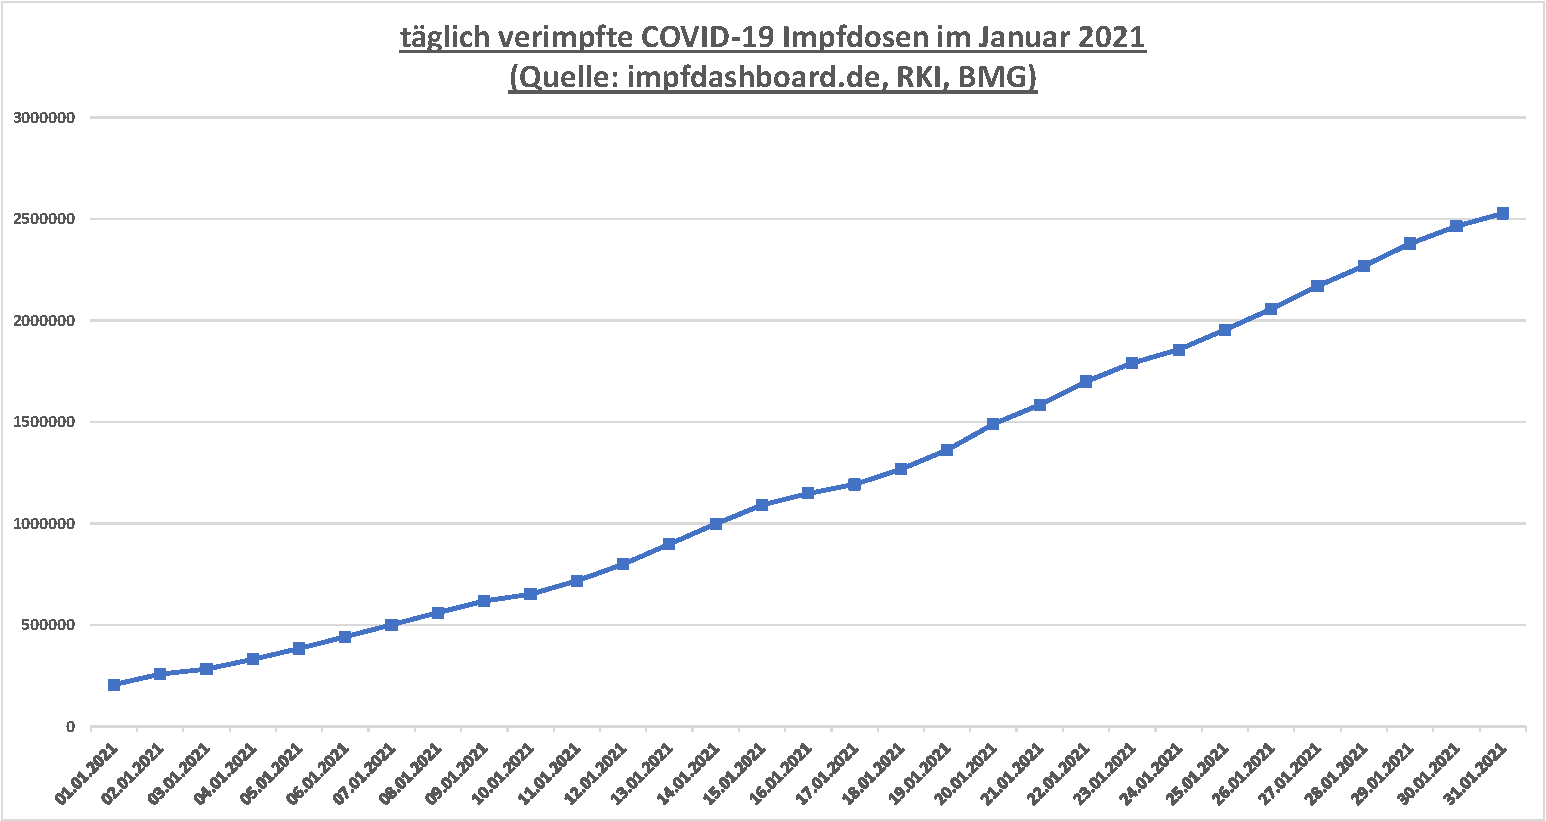
\includegraphics[width=\textwidth]{graphics/Beispiel-Zeitreihe.pdf}
\caption{Beispielhafte Zeitreihe aus dem Januar 2021}
\label{abb:BeispielZeitreihe}
\end{figure}

Die möglichen Anwendungen in der Informatik sind ebenfalls vielzählig. So können über virtuelle oder physikalische Sensoren Messwerte, wie beispielsweise die CPU Auslastung eines gegebenen Servers über die Zeit oder Temperaturmessungen eines \ac{IoT} Gerätes über die Zeit gemacht und gespeichert werden.

Ein wichtiges Merkmal von Zeitreihen ist die Distanz zwischen den Messwerten, im Sinne der Messfrequenz, in welcher Daten betrachtet werden. \Todo{belegen} Ist eine Zeitreihe äquidistant, wurde mit gleichbleibender Frequenz gemessen und die zeitliche Distanz zwischen einzelnen Messwerten ist gleich. Für die in dieser Arbeit diskutierten Auswertungsarten wird eine Äquidistanz der gemessenen Daten angenommen, da andernfalls ein Bias bei der Analyse nicht ausgeschlossen werden kann. Gleichfalls ist es technisch möglich einzelne, nicht äquidistante Messwerte auszusortieren. Die in \autoref{abb:BeispielZeitreihe} abgebildete Zeitreihe ist äquidistant, da die Werte einmal am Tag gesammelt erhoben wurden.


\Todo{Definition Zeitreihendaten}
\Todo{Definition Datenanalyse}

Bei der Verarbeitung von Daten ist zu beachten, dass der Wert, bzw. die Erkentnisse die aus den Daten abgleitet werden können, über die Zeit reduziert wird. \footcite[Vgl. auch im Folgenden][]{NucleusResarchInc..2012} Gemäß \citeauthor{NucleusResarchInc..2012} haben dabei verschiedene Unternehmen verschiedene Zeiträume, in denen Daten nützlich sind, da sie sich in eine von drei Entscheidungstempos einkategorisieren lassen.\footcite[Vgl. auch im Folgenden][3]{NucleusResarchInc..2012} Die Entscheidungstempos sind taktisch, operativ und strategisch. Beim taktischen Entscheidungstempo werden Änderungen sehr schnell, nahe Echtzeit getroffen und implementiert. Im Gegensatz dazu werden Entscheidungen der operativen und strategischen Entscheidungstempi respektive erst in Tagen bzw. Wochen oder innerhalb einem Quartal oder länger implementiert. Je nach Entscheidungstempo sind Analysen von eingehenden Daten also wesentlich früher notwendig oder können beispielsweise auch nur einmal täglich erstellt werden.

% \footcite[Vgl. auch im Folgenden][3]{NucleusResarchInc..2012}
% The value of data diminishes based on the cadence of decisions. Decision tempos are
% tactical (driving process changes in near real time), operational (driving changes that take
% days or weeks to implement), or strategic (driving changes that become part of a quarterly
% or longer planning and implementation process). The concept of half life, with diminishing
% value curves based on a company’s decision tempo, can be used to help companies
% measure the impact of prioritizing their data management and analytics investments. 



Für Unternehmen mit taktischem Entscheidendungstempo haben, gemäß der in \autoref{abb:DataHalflife} gezeigten Befragungsergebnisse von \citeauthor{NucleusResarchInc..2012}, Daten nach maximal 30 Minuten die Hälfte des Wertes eingebüßt.\footcite[Vgl. auch im Folgenden][6]{NucleusResarchInc..2012} Für operative Entscheidungstempi ist die durchschnittliche Halbwertszeit nach acht Stunden erreicht, für strategische Entscheidungstempi nach ca. 56 Stunden, also nach über 2 Tagen.



\begin{figure}[H]
\centering
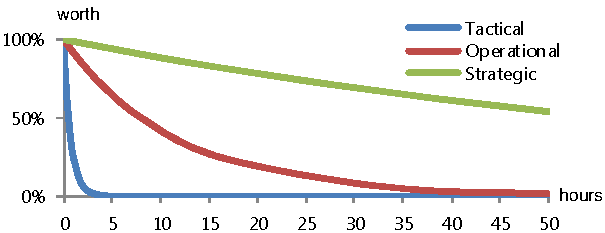
\includegraphics[width=\textwidth]{graphics/half-life-data.pdf}
\caption[Die Halbwertszeit von Daten]{Die Halbwertszeit von Daten\footnotemark}
\label{abb:DataHalflife}
\end{figure}
\footnotetext{Mit Änderungen entnommen aus: \cite{NucleusResarchInc..2012}}
Aus diesen abweichenden Halbwertszeiten und damit aus den abweichenden Zeiträumen, in denen die erhobenen Daten den höchsten Wert haben, ergibt sich die Notwendigkeit von verschiedenen Datenverarbeitungsstrategien, um entsprechend strategischen, taktischen und operativen Entscheidenden die werthaltigsten Daten als Entscheidungsgrundlage zu präsentieren.

\subsection{Arten der Auswertung}
Diese Arbeit soll anhand einiger weniger Auswertungen demonstrieren, wozu die jeweilige Referenzarchitektur und die verwendeten Dienste fähig sind. Im Folgenden werden dazu einige einfachere Auswertungsmethoden für Zeitreihendaten vorgestellt. Die Zeitreihenanalyse und einsetzbare Werkzeuge werden im statistischen Sinn von weiterführenden Werken, wie von \citeauthor{Shumway.2017} behandelt. Es ist davon auszugehen, dass auch weiterführende Auswertungen wie fourieranalytischen Methoden, sofern in der jeweiligen Umgebung bereits vorhanden oder programmierbar, eingesetzt werden können.
\subsubsection{Median}
\begin{tikzpicture}
    \begin{axis}[
    xlabel=Zeit (Minuten),
    ylabel=Messwert,
    xmin=0, 
    ymin=0,
    legend pos=outer north east]
        \addplot {sin(deg(x-1.6))+1}; 
        \addplot {0.5899082};
        \addplot {1.2392493};
        \addplot {1.72939505};
        \legend{$\sin(x-1.6)+1$,25stes Perzentil,Median,75tes Perzentil}
    \end{axis}
\end{tikzpicture}


\subsubsection{Anomaliedetektion}
\begin{tikzpicture}
    \begin{axis}[
    xlabel=Zeit (Minuten),
    ylabel=Messwert,
    xmin=0, 
    ymin=0,
    legend pos=outer north east]
        \addplot {sin(deg(x-1.6))+1}; 
        \addplot {2*sin(1.5*deg(x-1))+2};
        \addplot {0.5*sin(2*deg(x-1.6))+1};
        \legend{Normaler Verlauf,Anomalie 1,Anomalie 2}
    \end{axis}
\end{tikzpicture}

\subsubsection{Schwellwertüberschreitung}

\begin{tikzpicture}
    \begin{axis}[
    xlabel=Zeit (Minuten),
    ylabel=Messwert,
    xmin=0, 
    ymin=0,
    legend pos=outer north east]
        \addplot {sin(deg(x-1.6))+1}; 
        \addplot {1.75};
        \draw [line width=0.8mm, black](axis cs:3,0) -- node[right]{Karenzzeit} (axis cs:3,2);
        \legend{$\sin(x-1.6)+1$,Schwellwert ($1.75$)}
    \end{axis}
\end{tikzpicture}

\subsubsection{Trenderkennung/gleitender Durchschnitt}


% \Todo{Grafik Data Analytics Pipeline}
\begin{figure}[H]
\centering
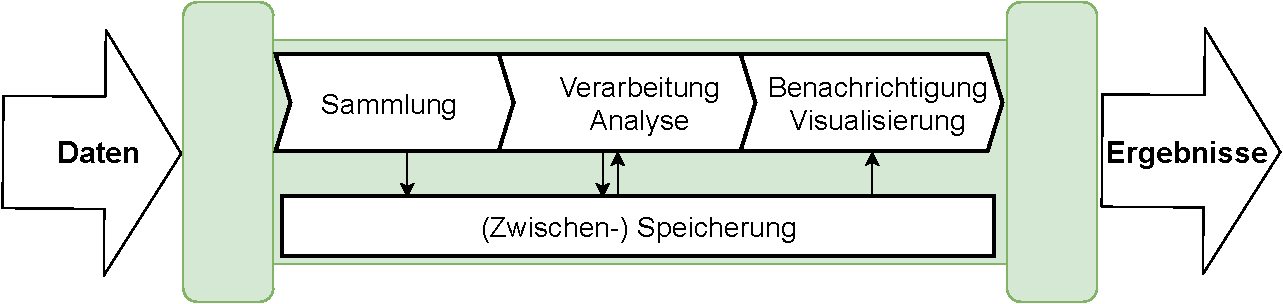
\includegraphics[width=\textwidth]{graphics/DataPipeline.pdf}
\caption{Aufbau und Ablauf in einer Data Pipeline}
\label{abb:DataPipeline}
\end{figure}
\Todo{Quellenangabe}


\subsection{Bestehende Referenzarchitekturkategorien}
Im Bereich der Streamingarchitekturen gibt es bereits etabblierte Referenzarchitekturen, welche verschiedene mögliche Aufbauarten einer Verarbeitung von Streaming/Zeitseriendaten zeigen.

% \Todo{Lambda, Kappa, OLAP elaborieren}
\begin{figure}[H]
\centering
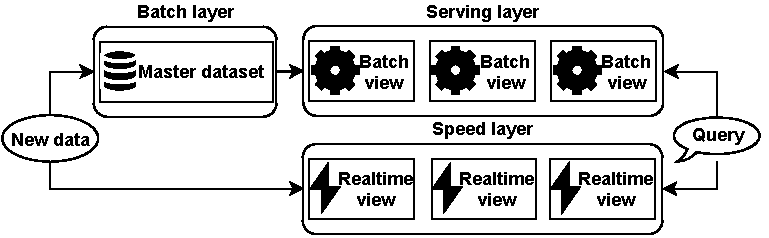
\includegraphics[width=\textwidth]{graphics/Lambda-Reference-Architecture.pdf}
\caption[$\lambda$-Datenstreaming Referenzarchitetktur]{$\lambda$-Datenstreaming Referenzarchitetktur.\footnotemark}
\label{abb:LambdaStreaming}
\end{figure}
\footnotetext{Mit Änderungen entnommen aus: \cite[][28]{Marz.2015}}
% Lambda nach \citeauthor{Marz.2015}, siehe \footcite[Vgl.][28]{Marz.2015}

Die von \citeauthor{Marz.2015} vorgestellte $\lambda$/Lambda-Architektur, welche in \autoref{abb:LambdaStreaming} gezeigt wird ist dabei eine der sehr bekannten Referenzarchitekturen. Der Name ist dabei nicht mit dem \ac{AWS} Dienst Lambda zu verwechseln, sondern ist wohl auf den gedrehten Buchstaben $\lambda$ zurückzuführen, also \reflectbox{\rotatebox[origin=c]{270}{$\lambda$}}.\footcite[Vgl. auch im Folgenden][]{Berle.27.11.2017} Die $\lambda$-Architektur sieht ausgehend von den hereingeladenen Daten zwei verschiedene Wege für die Daten vor. Zum einen den \enquote{Speed Layer}, welcher Daten direkt nach Eingang verarbeitet und nicht im Layer selbst speichert, sondern nur Aggregate oder Ergebnisse zur Verfügung stellt. Zum anderen gibt es den \enquote{Batch layer}, in welchem Daten zuerst in einem Master dataset gespeichert werden und dann in einem festen Intervall (\enquote{Batch jobs}) ausgewertet werden. Verschiedene Datenverarbeitungsintervalle machen speziell im Sinne der verschiedenen, in \autoref{abb:DataHalflife} gezeigten, Datenhalbwertszeiten Sinn. So sind manche Auswertungen, die präzise historische Daten benötigen in einem Batch layer besser möglich als in einem speed layer. Der speed layer bietet dagegen durch die Geschwindigkeit der Auswertungen die möglichkeit, agil auf erkannte Ereignisse oder Veränderungen im generellen zu reagieren.


\begin{figure}[H]
\centering
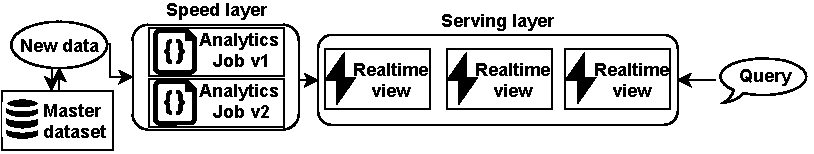
\includegraphics[width=\textwidth]{graphics/Kappa-Reference-Architecture.pdf}
\caption[$\kappa$-Datenstreaming Referenzarchitetktur]{$\kappa$-Datenstreaming Referenzarchitetktur.\footnotemark}
\label{abb:KappaStreaming}
\end{figure}
\footnotetext{Mit Änderungen entnommen aus: \cite{Kreps.2014}, \cite{Berle.27.11.2017}}

Die $\kappa$/Kappa Referenzarchitektur von \citeauthor{Kreps.2014}, dargestellt in \autoref{abb:KappaStreaming} basiert auf der $\lambda$-Architektur, spart jedoch den \enquote{Batch layer} mit zugehörigen \enquote{Batch jobs} aus. Das Konzept von Master Data existiert dabei weiterhin, jedoch in Form von Nachrichten, die in einem Messagebroker gespeichert werden. Analysen werden in Form von einzelnen, unveränderlichen Jobs über die vorhandenen Nachrichten erstellt. Wird die Analyse in irgendeiner Weise verändert (z.B. durtch Codeanpassungen) werden alle zwischengespeicherten Nachrichten erneut durch eine neue, unveränderliche Version des Jobs analysiert. Diese Unveränderlichkeit hat den Vorteil, dass keine unerwünschten Seiteneffekte durch Analysen, die gegenseitig Ergebnisse überschreiben auftreten. \Todo{elaborate on original source}

% Kappa nach \citeauthor{Kreps.2014},
% siehe \footcite[Vgl.][]{Kreps.2014}



\begin{figure}[H]
\centering
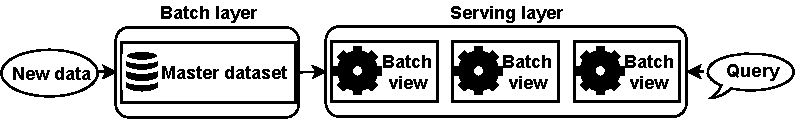
\includegraphics[width=\textwidth]{graphics/OLAP-Reference-Architecture.pdf}
\caption[OLAP Referenzarchitetktur]{OLAP Referenzarchitetktur.\footnotemark}
\label{abb:OLAPStreaming}
\end{figure}
\footnotetext{Mit Änderungen entnommen aus: \cite{Kreps.2014}}

%\ac{OLAP}
Aus der $\lambda$ Referenzarchitektur lässt sich auch eine, zur $\kappa$ Architektur gegenteilige Architektur aufzeigen, welche ein klassisches \ac{OLAP} Szenario aufzeigt. \Todo{Codd zitieren} Diese Architektur basiert, wie in \autoref{abb:OLAPStreaming} gezeigt, auf einer periodischen Verarbeitung der Daten im Master dataset. Dieses Vorgehen ist bei traditionellen Analytics weit verbreitet, bietet jedoch womöglich wichtige Einsichten erst nachdem die Datenhalbwertszeit bereits überschritten wurde.



\subsection{Echtzeitverarbeitung}
Gemäß der in \autoref{abb:KappaStreaming} gezeigten $\kappa$-Architektur gibt es Nutzungsfälle, in welchen eine reine Echtzeitauswertung basierend auf einer Datenquelle, wie beispielsweise dem Messagebroker Sinn machen kann. \citeauthor{Belur.2020} sieht dabei vier verschiedene Verwendungszwecke, in welchen die niedrige Verarbeitungslatenz besonders wichtig ist und den maximalen Wert aus den Daten zieht.\footcite[Vgl. auch im Folgenden][]{Belur.2020} Durch Echtzeit reporting und die Erstellung von Dashboards können aktuelle Daten schnell übersichtlich aufbereitet werden. Mittels erstellter Regeln, die Schwellwertüberschreitungen und Anomalien detektieren, können Nutzende benachrichtigt werden, sobald es zu einer Abweichung kommt. Ebenfalls sinnvoll ist Machine Learning zum auffinden von Mustern in den Daten zu verwenden, was verbesserte Anomalierkennung, Vorraussagen und ähnliche Features ermöglicht. Ein weiterer valider Usecase der $\kappa$-Architektur ist die Transformation von Daten in gewisse Zielformate, um beispielsweise Drittsysteme anzusprechen.
Requirements:
\begin{itemize}
\item Unified experience for data ingestion and edge processing
\item Versatile out-of-the-box connectivity
\item Scalable stream processing with complex transformations
\item Operationalized business rules and ML models
\item Ability to handle unstructured data and schema drift:
\item Reusability of processing logic
\item Governance and lineage
\end{itemize}

% \subsubsection{Streamanalyse}
% \begin{itemize}
% \item AWS Kinesis Data Analytics/Stream
% \item AWS Lambda
% \end{itemize}

\subsection{Datenbankseitige Verarbeitung}
% \subsubsection{Datenbankabfragen}
% \begin{itemize}
% \item Timestream
% \item Redshift
% \item Athena
% \item Elasticsearch
% \end{itemize}

% \subsubsection{Externe Analyse}
% \begin{itemize}
% \item Amazon EMR
% \item Amazon Glue
% \item AWS Lake Formation
% \end{itemize}
Gemäß der in \autoref{abb:OLAPStreaming} gezeigten \ac{OLAP} Architektur, gibt es, wie für die Echtzeitverarbeitung auch nutzende Unternehmen, die ein Entscheidugnstempo mit höherem Horizont haben. Für diese Entscheidungstypen ist dabei wichtig, dass eine Analyse möglichst viele historische Daten umfasst, aber nicht so wichtig, wie zeitnah diese erstellt werden kann. Eine gängige Möglichkeit um effizient alte Daten zu analysieren stellen \ac{OLAP} Datenbanken dar, welche durch spezielle Indexstrukturen und Optimierungen auf komplexe lesende Abfragen bei großen Datenmengen optimiert wurden. \Todo{belegen} Mittels dieser \ac{OLAP} Datenbanken lassen sich dank der jeweiligen Abfragesprachen und -dialekte komplizierte Abfragen realisieren. Bekanntes Beispiel für so eine Abfragesprache wäre \ac{SQL}, welches einige verschiedene Implementierungen (Dialekte) hat, die verwendet werden können. 


NOTIZEN:
Source -> Stream ingestion -> Stream storage -> Stream processing -> Destination

Talkingpoints gegen Streaming onprem:
Difficult to set up, Difficult to achieve high availability,
Error prone and complex to manage,
Tricky to scale, Integration requires development,Expensive to maintain

Amazon Kinesis Data Streams - Daten verfügbar in 70 Milisekunden

Amazon Kinesis Data Analytics

\section{Referenzarchitektur}\label{theorie:referenzmodellierung}
Nach \citeauthor{Bass.2010} ist eine Referenzarchitektur ein spezialisiertes Referenzmodell, wie in \autoref{abb:RelationshipsReferenceModel} gezeigt, welche in Softwarearchitekturen instanziiert werden kann. \footcite[Vgl.][S.~17~f.]{Bass.2010} 

\begin{figure}[H]
\centering
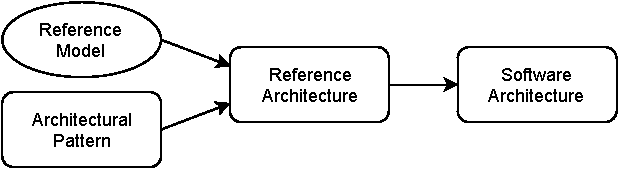
\includegraphics[width=0.66\textwidth]{graphics/Relationships-reference-models.pdf}
\caption[Beziehungen zwischen Referenzmodellen, Architekturpatterns, Referenzarchitekturen und Softwarearchitekturen]{Beziehungen zwischen Referenzmodellen, Architekturpatterns, Referenzarchitekturen und Softwarearchitekturen.\footnotemark}
\label{abb:RelationshipsReferenceModel}
\end{figure}
\footnotetext{Mit Änderungen entnommen aus: \cite[][18]{Bass.2010}}

In diesem Kapitel sollen deshalb die theoretische Definition des Referenzarchitekturbegriffs, genauso wie mögliche Vorgehensmodelle betrachtet werden.



\subsection{Referenzmodelle}

Gemäß des konstruktionsprozessorientierten Referenzmodellbegriffs von \citeauthor{vomBrocke.2003} ist ein Referenzmodell als solches zu erkennen, wenn der Gegenstand und/oder\footnote{Die Verwendung von \enquote{und/oder} wurde hier gewählt, da der Autor der Quelle das \enquote{oder} aus der boolschen Algebra gewählt hat um explizit beide Fälle einzuschliessen.} der Inhalt des Referenzmodells bei der Konstruktion des Gegenstandes und/oder des Inhaltes eines zu konstruierenden Anwendungsmodells wiederverwendet werden kann.\footcite[Vgl.][34]{vomBrocke.2003} Dabei hat ein Referenzmodell einen Empfehlungscharakter und stellt eine \enquote{best practice} dar.\footcite[Vgl.][31]{vomBrocke.2003} 

Ein Referenzmodell kann nach \citeauthor{vomBrocke.2003} nicht objektiv allgemeingültig sein und auch keinen objektiven Empfehlungscharakter haben, sondern muss subjektiv beurteilt werden.\footcite[Vgl. auch im Folgenden][31~f.]{vomBrocke.2003}  Dabei ist zumindest von den Interessensgruppen der Konstruierenden und der Nutzenden auszugehen, welche das Referenzmodell subjektiv unterschiedlich nach Allgemeingültigkeit und Empfehlungscharakter bewerten. Je nachdem welche Beurteilung höher gewichtet wird und früher einfließt, kann also entweder von der Situation ausgegangen werden, dass das Referenzmodell vom Konstruierenden zu einem solchen erklärt wird oder ein Modell, ob vom Konstruierenden beabsichtigt oder nicht, von den Nutzenden zu einem solchen erhoben wird.


\subsection{Referenzarchitektur}
Der IEEE Standard 1471-2000 definiert Architektur im Kontext von softwareintensiven Systemen wie folgt:
\enquote{The fundamental organization of a system embodied in its components, their relationships
to each other, and to the environment, and the principles guiding its design and evolution.} \footcite[][3]{IEEEComputerSociety.2000}. Als softwareintensives System kann jedes System gesehen werden, bei dem Software essentielle Einflüsse auf das Design, die Erstellung, das Deployment oder die Evolution des Systems hat.\footcite[Vgl.][1]{IEEEComputerSociety.2000}

Wird dieser Architekturbegriff auf bekannte Bereitstellungsmodi aus der Cloud, wie \ac{SaaS}, \ac{PaaS}, \ac{IaaS} oder \ac{FaaS} angewendet, wird klar, dass von einer Architektur im Sinne des IEEE Standards 1471-2000 ausgegangen werden kann, sobald Software involviert ist. Im Rahmen dieser Arbeit werden auch Dienste, die sich nach der NIST Cloud Definition unter \ac{SaaS} Dienste zählen lassen, behandelt. Als \ac{SaaS} Dienst gilt dabei jeder Dienst, bei dem Nutzende die unterliegende Infrastruktur nicht verwalten und die Applikation nur über limitierte Konfigurationen verwalten können. Sollte aber die Konfiguration mittels einer Programmiersprache bzw. Datenabfragesprache wie \ac{SQL} erfolgen, ist die Bedingung erfüllt, dass Software wesentliche Einflüsse auf das System hat.


\citeauthor{Gallagher.2000} definiert eine Referenzarchitektur als eine generalisierte Architektur mehrerer Endsysteme, die eine oder mehrere Domänen teilen.\footcite[Vgl. auch im Folgenden][3]{Gallagher.2000} Die Referenzarchitektur definiert nach Sicht des Autors dabei die gemeinsame Infrastruktur der Endsysteme und die Schnitstellen der Komponenten, die in den Endsystemen enthalten sein sollen. Dabei ist eine Referenzarchitektur zu instanziieren, um eine spezifische Softwarearchitektur zu erstellen. Gallagher definiert die Aufgaben einer Referenzarchitektur wie folgt: Zum einen werden übergreifende Funktionen und Konfigurationen generalisiert und extrahiert und zum anderen wird eine kosteneffiziente und verlässliche Basis geschaffen, um Zielsysteme abzuleiten/zu instanziieren.\footcite[Vgl.][3]{Gallagher.2000}

\citeauthor{Trefke.2012} schränkt in seiner Definition die Instanziierung insoweit ein, dass individuelle Besonderheiten abstrahiert werden müssen, um eine Allgemeingültigkeit der Referenzarchitektur in einer speziellen Domäne zu erhalten.  \footcite[Vgl. auch im Folgenden][]{Trefke.2012} Zusätzlich fügt \citeauthor{Trefke.2012} der Referenzarchitektur als optionale Aufgaben die Definition von Leitlinien für die Verwendung, Evolution und Verantwortlichkeiten hinzu. Zurückgreifend auf \citeauthor{vomBrocke.2003} legt \citeauthor{Trefke.2012} fest, dass eine Referenzarchitektur als spezifischeres Referenzmodell seinen Empfehlungscharakter entweder durch Erfahrungen und hohe Nutzerakzeptanz oder durch Festsetzung von Erschaffenden erhält.

Nach \citeauthor{Angelov.2012} gibt es zwei Typen und damit verbundene Zielsetzungen der Referenzarchitektur: Die standardisierende Referenzarchitektur, welche darauf zielt eine Standardarchitektur für spezielle Anwendungsfälle zu schaffen und die unterstützende/erleichternde Referenzarchitektur, welche Personen in Architekturrollen unterstützen sollen, ähnliche Probleme leichter zu lösen.\footcite[Vgl. auch im Folgenden][S.~422~ff.]{Angelov.2012} Nach \citeauthor{Angelov.2012} sind standardisierende Referenzarchitekturen nicht zur Verwendung von innovativen, also kaum getesteten oder noch nicht von Experten akzeptierten Elementen geeignet. Die unterstützenden/erleichternden Referenzarchitekturen hingegen können solche innovativen Elemente durchaus verwenden und auch eine Technologievorauswahl treffen.

Um einen möglichst hohen Nutzen stiften zu können, müssen die organisatorischen Rahmenbedingungen, in welchen ein Referenzmodell eingesetzt werden soll, analysiert werden.\footcite[Vgl.][]{vomBrocke.2004}

%\Todo{What are inputs of a Reference Architecture? - Muller.2020}
\citeauthor{Muller.2020} empfiehlt, eine Referenzarchitektur zur Generalisierung von vorhandenen Architekturen zu verwenden.\footcite[Vgl. auch im Folgenden][7]{Muller.2020} Für neue Technologien und Applikationen, die bislang in der Form kaum verwendet wurden, schlägt \citeauthor{Muller.2020} stattdessen ein inkrementelles Vorgehen vor. Das inkrementelle Vorgehen von \citeauthor{Muller.2020} beinhaltet dabei die Erstellung von Prototypen und Einholung von Feedback der Zielstakeholder. 


\subsection{Diskussion der Qualitätskriterien der Referenzarchitekturen}\label{chap:qualitycriteria}
\citeauthor{Muller.2020} schlägt sieben Qualitätskriterien vor, welche von einer guten Referenzarchitektur erfüllt werden sollten:\footcite[Vgl. auch im Folgenden][8]{Muller.2020}
\begin{enumerate}
\item Verständlichkeit für eine breite, heterogene Gruppe an Stakeholdern (Kunden, Projektmanager, Entwickler, etc.)
\item Zugänglichkeit und Zugriff durch die Mehrheit der Organisation
\item Adressierung der Hauptprobleme der spezifischen Problemdomäne
\item Zufriedenstellende Qualität
\item akzeptabel
\item \enquote{up-to-date} und wartbar
\item wertschöpfend für den Betrieb
\end{enumerate}

\ac{AWS} definiert im Rahmen des sogenannten Well Architected Frameworks für verschiedene \enquote{Lenses}, also Spezialisierungen, Themenfelder, die bei exzellenten Architekturen zu beachten sind. Für Datenanalysen gibt es die Analytics Lens, welche entsprechend für Referenzarchitekturen genauso Anwendung finden sollte. Kriterien sind dabei die Folgenden:\footcite[Vgl.][6]{Ravirala.2020}:
\begin{enumerate}
\item Automate data ingestion
\item Design ingestion for failures and duplicates => Siehe Robustness and fault tolerance
\item Preserve original source data
\item Describe data with metadata
\item Establish data lineage
\item Use the right ETL tool for the job
\item Orchestrate ETL workflows
\item Tier storage appropriately
\item Secure, protect, and manage your entire analytics pipeline
\item Design for scalable and reliable analytics pipelines => Scalability, robustness and fault tolerance
\end{enumerate}


\subsection{Vorgehensmodell}

\citeauthor{Schutte.1998} unterteilt Referenzmodellierung generell in vier Phasen.\footcite[Vgl. auch im Folgenden][184\psq]{Schutte.1998} Die erste Phase, die Problemdefinition ist mit der Darstellung des behandelten Problems in der Einleitung dieser Arbeit bereits vorgenommen worden. Laut \citeauthor{Schutte.1998} kann der Wirklichkeitszugang des erstellten Modells nur über Bilder erfolgen, welche entsprechend zu modellieren sind.\footcite[Vgl. auch im Folgenden][185\psq]{Schutte.1998} Da momentan keine Erfahrungen in den zu verwendenden Technologien für die Referenzmodellierung vorliegt, handelt es sich um eine Top-down Referenzmodellierung/Referenzarchitektur. Bei der Konstruktion des Referenzmodellrahmens wird durch das \enquote{Was} motiviert, welche Unternehmensspezifika zu beachten sind.\footcite[Vgl. auch im Folgenden][186]{Schutte.1998} In der vorliegenden Arbeit wäre beispielsweise Teil des Referenzmodellrahmens, dass cloudbasiert gearbeitet werden soll und dass die Zeitreihendaten vorerst vornehmlich von \ac{IoT} Anwendungsfällen stammen, was sich später dennoch ändern könnte.\footcite[Vgl. auch im Folgenden][187\psq]{Schutte.1998} In der \enquote{Wie} Phase, die dieses Kapitel behandeln soll, wird die Referenzarchitektur strukturiert und Darstellungsarten gezeigt, welche folgend angewendet werden können. 

\begin{figure}[H]
\centering
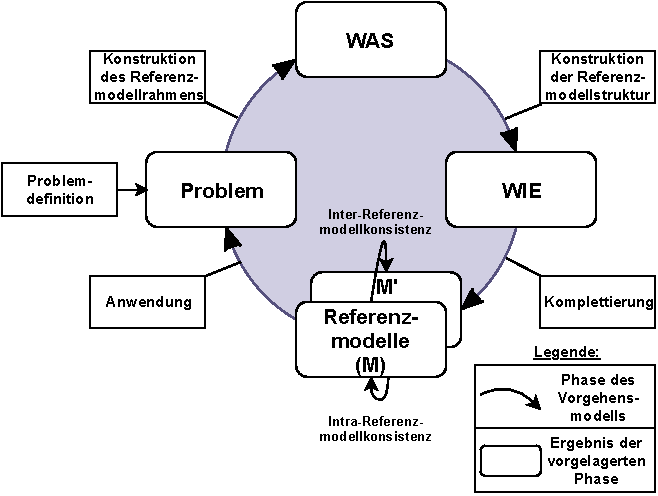
\includegraphics[width=0.75\textwidth]{graphics/Vorgehen-Referenzmodellierung.pdf}
\caption[Vorgehensmodell Referenzmodellierung nach Schütte]{Vorgehensmodell Referenzmodellierung nach Schütte.\footnotemark}
\label{abb:VorgehensmodellReferenzmodellierung}
\end{figure}
\footnotetext{Mit Änderungen entnommen aus: \cite[][185]{Schutte.1998}}




Nach \citeauthor{Muller.2020} hat eine Referenzarchitektur mehrere Dekompositionen, in beispielsweise eine funktionale, eine konstruktionsorientierte oder eine infrastrukturorientierte Komposition.\footcite[Vgl.][7]{Muller.2020} Diese Dekompositionsschichten lassen sich ebenfalls in bekannten Architekturframeworks wie arc42 finden, weshalb diese mit Anpassungen zur Visualisierung dienen sollen. Dies deckt sich auch mit der Auffassung von \citeauthor{Schutte.1998} zur Referenzmodellierung, welcher Modellierung über Bilder erfolgen lassen möchte.\footcite[Vgl.][185]{Schutte.1998}

\begin{figure}[H]
\centering
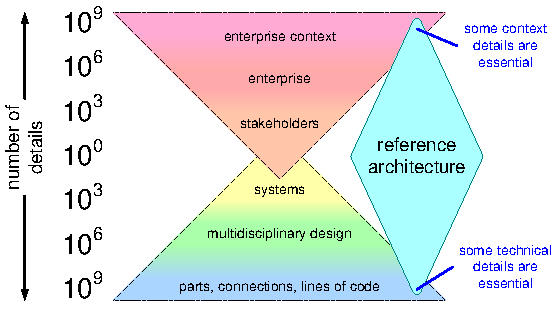
\includegraphics[height=0.23\textheight]{graphics/reference-architecture-details.pdf}
\caption[Gewünschter Detailgrad von Referenzarchitekturen nach \citeauthor{Muller.2020}]{Gewünschter Detailgrad von Referenzarchitekturen nach \citeauthor{Muller.2020}.\footnotemark}
\label{abb:DetailgradMuller}
\end{figure}
\footnotetext{Entnommen aus: \cite[][11]{Muller.2020}}

Mehrere Dekompositionen machen insbesondere auch Sinn, da wie im Diagramm von \citeauthor{Muller.2020} - \autoref{abb:DetailgradMuller} - eine Addressierung von unterschiedlichen Aspekten wie Systemgestaltung, aber auch Stakeholder oder Kontext erfolgen sollte. Eine Adressierung der Stakeholder und des Kontextes ist insofern gegeben, dass, wie in \autoref{chap:requirements} gezeigt, Interviews durchgeführt und im Anhang dieser Arbeit transkribiert werden. An Stellen, an denen ein Einsatz von Teilen der Referenzarchitektur nontrivial scheint, kann durch Codebeispiele oder konkrete, kopierbare \enquote{Schnipsel} gezeigt werden, auf was speziell im technischen Bereich zu achten ist.

Zusätzlich sollen Dekompositionen unterschiedliche Aufgaben erfüllen. Speziell für die Darstellung der verwendeten Diensten von \ac{AWS} in den Referenzarchitekturen und dem Datenfluss soll die erste Stufe der Bausteinsicht des Architekturstandards arc42 verwendet werden. Das Konzept jener Bausteinsicht, also wie sie zu gestalten ist, findet sich in \autoref{abb:BausteinsichtStufe1}. In der finalen Umsetzung werden die offiziellen \ac{AWS} Icons die entsprechenden Services darstellen, die verwendet werden.

\begin{figure}[H]
\centering
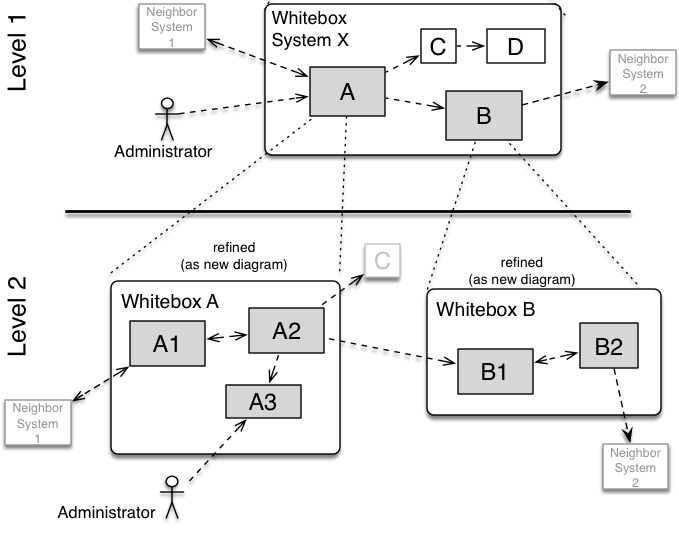
\includegraphics[height=0.38\textheight]{graphics/Bausteinsicht.png}
\caption[Stufe 1 der Bausteinsicht in arc42]{Stufe 1 der Bausteinsicht in arc42.\footnotemark}
\label{abb:BausteinsichtStufe1}
\end{figure}
\footnotetext{Mit Änderungen entnommen aus: \cite{Starke.o.J.}}

Zusätzlich zu der Bausteinsicht können, wie in \autoref{abb:Diagrammtypen} geizeigt, weitere Diagrammtypen eingesetzt werden, um verschiedene Dekompositionen darstellen zu können.

\begin{figure}[H]
\centering
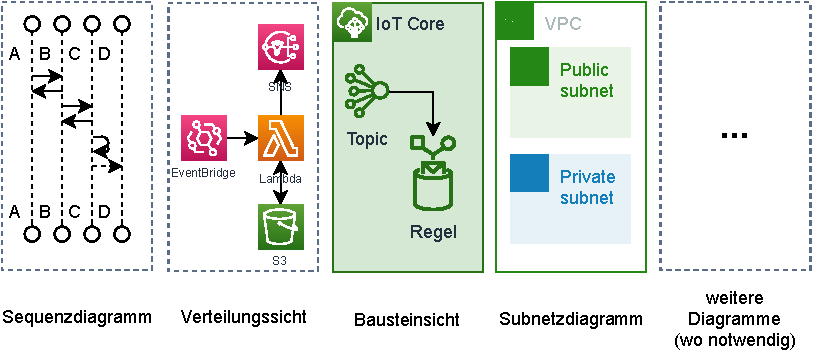
\includegraphics[width=\textwidth]{graphics/Diagrammtypen.pdf}
\caption{Ergänzende Dekompositionen}
\label{abb:Diagrammtypen}
\end{figure}


Wie von \citeauthor{Muller.2020} vorgeschlagen und im vorherigen Unterkapitel erläutert, ist ein inkrementeller Ansatz unter Verwendung von Prototypen und kontinuierlichem Feedback der Zielstakeholder unerlässlich.\footcite[Vgl.][7]{Muller.2020} 

Sehr wichtig für eine Referenzarchitektur ist auch die Dokumentation, wie die Wiederverwendung zu handhaben ist. Ein möglicher Ansatz wäre dabei die gezielte Integration und Dokumentation von Variationspunkten, wie von \citeauthor{Webber.2001} vorgeschlagen.\footcite[Vgl.][24\psqq]{Webber.2001} Mittels der Variationspunkte kann eine statische Referenzarchitektur konstruiert werden, welche an spezifisch definierten Punkten angepasst werden muss, um einzigartige Architekturen zu erzeugen.\footcite[Vgl.][24]{Webber.2001} Dabei gibt es vier verschiedene Ansichten, aus denen Variationspunkte definiert werden können:\footcite[Vgl.][25\psq]{Webber.2001}
\begin{enumerate}
\item \label{view:first} Requirement-Variation-Point View
\item \label{view:second} Component-Variation-Point View
\item \label{view:third} Static-Variation-Point View
\item \label{view:fourth} Dynamic-Variation-Point View
\end{enumerate}
Dabei sind für diese Arbeit, in der keine implementierungsnahe (im Sinne von Programmierung) Softwarearchitektur entworfen wird, hauptsächlich die anforderungsbasierte und die komponentenbasierte Variationspunktsicht aus \autoref{view:first} und \autoref{view:second} wichtig. Die statische und dynamische Variationspunktsicht aus \autoref{view:third} und \autoref{view:fourth} agieren stärker auf Implementierungsebene.\footcite[Vgl. auch im Folgenden][25\psq]{Webber.2001} Auf dieser können beispielsweise mittels objektorientierter Programmierung Klassen bereitgestellt werden, von welchen geerbt werden kann. Gleichzeitig kann die Verhaltensweise des Programms auch durch z.B. Callbacks oder Parameterisierung des Aufrufes verändert werden.

\renewcommand\#{\protect\scalebox{0.8}{\protect\raisebox{0.4ex}{\char"0023}}}

Variationspunkte können, wie in \autoref{abb:Variationspunkte} dargestellt innerhalb der verschiedenen, dargestellten Schichten wie folgt dargestellt werden:
\begin{figure}[H]
\centering

\includegraphics[height=1.33cm]{graphics/Variationpoints.pdf}
\caption{Darstellung Variationspunkte}
\label{abb:Variationspunkte}
\end{figure}
In den Architekturebenen werden entsprechend die Variationspunkte mit durchgängigen Nummern versehen, welche entsprechend vor dem \# stehen.





% Überleitung => generelle Referenzmodelle 
% => Empfehlungscharakter 
% => Anwendung Architektur 
% => Unterlegung Arc42 als Modellierungssprache



\section{Theorie der Anforderungserhebung}\label{chap:requirements}

Gemäß der in \autoref{chap:qualitycriteria} definierten Qualitätskriterien und der von \citeauthor{vomBrocke.2003} aufgestellten Allgemeingültigkeitskriterien kann ein Referenzmodell und damit auch eine Referenzarchitektur nicht objektiv allgemeingültig sein. Zusätzlich ergeben sich als weitere wichtige Eingaben zur Konstruktion eines Referenzmodells die Dekompositionstiefe und die Anwendbarkeit. Zusammen lassen sich diese Dimensionen als Kiviat Diagramm,\footcite[Vgl.][33\psqq]{Kolence.1973} wie in \autoref{abb:Dimensionen} gezeigt, abbilden. Die Dekompositionstiefe misst die Anzahl an Schichten und die Detailtiefe der verschiedenen Dekompositionsschichten die im Rahmen der Architektur verwendet werden. Ein niedriger Wert entspricht einer geringen Anzahl, welche keine große Detailtiefe aufweisen. In \autoref{abb:Diagrammtypen} sind mögliche Dekompositionen mit unterschiedlicher Tiefe gezeigt. Die Anwendbarkeit, als Gegensatz zur Abstraktion misst, wie gut und schnell sich eine Referenzarchitektur instanziieren lässt, um eine spezifische Architektur abzuleiten. Ein niedriger Wert bedeutet eine sehr abstrakte Referenzarchietktur, deren Instanziierung mit viel Aufwand verbunden ist. Die Allgemeingültigkeit beschreibt die Menge an Anwendungsfällen und die Losgelöstheit von Firmenspezifika beziehungsweise die übergreifende Gültigkeit in mehreren Teams. Idealerweise ist eine Referenzarchitektur spezifisch für eine Zielorganisation, aber nicht zu spezifisch, sondern erlaubt Anwendungen in anderen Teams.

\begin{figure}[H]
\centering
\scalebox{0.75}{
    \spider{0}{0}{0}
}

\caption{Referenzarchitekturdimensionen}
\label{abb:Dimensionen}
\end{figure}

Ziel einer Referenzarchitektur sollte also sein, das optimale Verhältnis der drei Dimensionen für die Zielstakeholder zu finden und daraus eine Referenzarchitektur zu erstellen. Um dieses Ziel zu erreichen, sind Interviews mit Zielstakeholdern der SPIRIT/21 zu führen, welche dem Interviewleitfaden in \autoref{tab:intervieleitfaden} folgen. Im referenzierten Leitfaden stehen dabei Fragen mit einem F-Präfix für allgemeine Fragen und Fragen mit einem D-Präfix für Fragen in Bezug auf die drei Dimensionen. Kombiniert mit mindestens einem Review der Referenzmodelle werden die Modelle zu einem nutzenstiftenden Artefakt.



\begin{table}[H]
\centering
\begin{tabular}{|l|l|}
\hline
ID & Beschreibung \\ \hline
\multicolumn{2}{|c|}{\cellcolor[HTML]{ECF4FF}Allgemeine Fragen} \\ \hline
F1 & Rolle innerhalb der SPIRIT/21 \\ \hline
F2 & Anwendungsgebiete der Referenzarchitekturen \\ \hline
F3 & Kompatibilität der Referenzarchitekturen zueinander? \\ \hline
\multicolumn{2}{|c|}{\cellcolor[HTML]{ECF4FF}Priorisierungen} \\ \hline
P1 & Priorisierung der Qualitätskriterien (siehe \autoref{chap:qualitycriteria}) \\ \hline
P2 & Priorisierung der Datennutzungstypen (siehe \autoref{chap:GrundlagenDatenanalyse}) \\ \hline
\multicolumn{2}{|c|}{\cellcolor[HTML]{ECF4FF}Dimensionen der Referenzarchitekturen} \\ \hline
D1 & Anforderungen an Anwendung der Referenzarchitekturen \\ \hline
D2 & Anforderungen an Allgemeingültigkeit der Referenzarchitekturen \\ \hline
D3 & Dekompositionstiefe der Referenzarchitekturen \\ \hline
\end{tabular}
\caption{Interviewleitfaden für Schlüsselstakeholder}
\label{tab:intervieleitfaden}
\end{table}




\section{Vergleichsmethodik für die Produktauswahl}\label{chap:vergleichsmethodik}

\citeauthor{Marz.2015}, die bereits die $\lambda$-Architektur geprägt haben, haben folgende,erwünschte Eigenschaften eines Big Data Systems festegelegt:\footcite[Vgl.][7\psqq]{Marz.2015}
\begin{enumerate}
\item Robustness and fault tolerance

Systeme sollen Herausforderungen, wie beispielsweise Paralellität, Datenduplikate oder technische Ausfälle verkraften. Zusätzlich ist Resilienz gegenüber menschlichen Fehlern wünschenswert, so dass händische Änderungen rückgängig gemacht werden können (also beispielsweise Analysecode \enquote{immutable} ist).
\item Low latency reads and updates

Lesezugriffe auf Daten sollen mit niedriger Latenz stattfinden. Wie bereits beschrieben, kann aufgrund der Messdistanz eine Aktualisierung von Daten durchaus längere Zeit benötigen, jedoch sollte ein Big Data System in der Lage sein, Datenaktualisierungen mit niedriger Latenz durchzuführen.
\item Scalability

Das Big Data System sollte durch transparente oder intransparente Provisionierung weiterer Ressourcen in der Lage sein, gleiche Performance in verschiedenen Belastungssituationen zu liefern. Dies deckt sich mit einem der Kernversprechen der Public Clouds nach NIST Definition (\enquote{rapid elasticity}).\footcite[Vgl.][2]{Mell.2011}
\item Generalization

Ein Big Data System sollte in der Lage sein, verschiedene Anwendungen zu unterstützen. Da die Zielsetzung dieser Bachelorarbeit auf Zeitreihendaten aufbaut, welche wie in \autoref{chap:GrundlagenDatenanalyse} gezeigt, einen großen Einsatzspielraum haben, ist diese Bedingung bei ausreichender Generalisierung der Referenzarchitekturen erfüllt.
\item Extensibility

Das zu gestaltende Big Data System soll erweiterbar sein und neue Funktionen oder Änderungen ohne größeren Aufwand ermöglichen.
\item Ad hoc queries

Diverseste Abfragen sollen schnellstmöglich auf dem Datensatz der Big Data Anwendung möglich sein.
\item Minimal maintenance

Eine Big data Anwendung soll wartbar bleiben, indem Komplexität in den Kernkomponenten, welche nach Ansicht von \citeauthor{Marz.2015} zu erhöhtem Wartungsaufwand führt, möglichst gering ist.
\item Debuggability

Innerhalb eines Big Data Systems soll es möglich sein, nachzuverfolgen, wie Werte entstanden sind, um mögliche Fehler verfolgen zu können.
\end{enumerate}

% Kriterien von Lukas an ein Produkt:
% \begin{itemize}
% \item zufriedenstellende Integration mit AWS nativen Diensten (z.B. Monitoring)
% \item Möglichst serverless (wenig Maintenance Aufwand)
% \item skalierbarkeit auf 0 bis 10000
% \end{itemize}

% Anforderungen von Kunden
% \begin{itemize}
% \item Skalierbarkeit
% \item pay for what you use (no dead infra)
% \item transparente Fehler
% \end{itemize}

% \begin{itemize}
%     \item Übertragbarkeit (ggf. zwischen Clouds)
% \end{itemize}

Vielleicht noch:
Requirements:\footcite[Vgl.][]{Belur.2020}
\begin{itemize}
\item Unified experience for data ingestion and edge processing
\item Versatile out-of-the-box connectivity
\item Scalable stream processing with complex transformations
\item Operationalized business rules and ML models
\item Ability to handle unstructured data and schema drift:
\item Reusability of processing logic
\item Governance and lineage
\end{itemize}

\subsection{Featurevergleich}
Es soll auf die Mindestverfügbarkeit folgender Fähigkeiten überprüft werden:
\begin{itemize}
\item Auswertungen nach \autoref{chap:auswertungsarten}
\end{itemize}

\subsection{Performancevergleich}
Es muss mindestens die theoretische Verarbeitungslatenz verglichen werden

\subsection{Kostenvergleich}
Um einen sinnvollen Kostenvergleich aufzustellen, sind folgende Annahmen zu treffen:
Es existieren 200 Geräte/Sensoren. Es geht eine Nachricht mit einem kB pro Minute pro Gerät ein (0,0432 GB/Gerät/Monat und 8,64 GB/Monat).
Es ist eine Vergleichsoperation auf einen Schwellwert auszuführen und wo möglich eine Zählung aller Schwellwertüberschreitungen der letzten drei Monate durchzuführen (historische Daten also mindestens 25,92 GB).  Es ist die Region Frankfurt (eu-central-1) mit Abrechnungswährung US-Dollar (Umrechnung in € erfolgt bei \ac{AWS} bei Abrechnung) zu wählen alternativ ist die Region Irland (eu-west-1) bei Nichtverfügbarkeit der Diensleistung in Frankfurt zu wählen. Produkte, die diese Analyse alleine nicht bewerkstelligen können, müssen unter zusätzlicher Verwendung von Rechendiensten wie Lambda oder \ac{EC2} angesetzt werden mit permanentem Speicher, der historische Daten speichert (\ac{S3}). Analysen, wo individuell auslösbar erfolgen alle 10 Minuten an Werktagen zwischen 9 und 17 Uhr, also monatlich 960mal. Andernfalls wird angenommen, dass der Schwellwert 5 mal pro Gerät pro Monat überschritten wird (1000 Überschreitungen).
Für die Zwischenspeicherung in \ac{S3}, wenn benötigt, wird folgendes Datenschema angenommen:

\begin{listing}[H]
\inputminted[frame=lines,breaklines=true]{json}{code/estimates/filtered-estimate.json}
\caption[Beispiel JSON]{Beispiel \ac{JSON}}
\label{listing:json}
\end{listing}
Um Historien über 3 Monate bereitzustellen, sind entsprechend 3000 Einträge nötig, was eine Dateigröße von ~455,32 KB ergibt. Das Berechnungsskript ist im Anhang \ref{anhang:berechnung} abgedruckt.


\begin{table}[H]
\centering
\begin{tabular}{|l|l|l|}
\hline
Dimension & Preis/Einheit           & Summe \\ \hline
Beispiel  & x\$/100.000 Datenpunkte & x\$  \\\hline
\end{tabular}
\caption{Kostenvergleich Schema}
\label{tab:kostenvergleich-schema}
\end{table}
Es sind alle Abrechnungsdimensionen in der in \autoref{tab:kostenvergleich-schema} gezeigten Form zu dokumentieren.






\chapter{Anwendungsfälle}

\section{Rahmenbedingungen der Datenverabeitung}\label{chap:rahmendatenverarbeitung}
Aufgrund bereits getroffener Architekturentscheidungen durch das \ac{IoT} Team der SPIRIT/21 GmbH wird für die Kommunikation zwischen Geräten und dem verarbeitenden Backend das \ac{MQTT} Protokoll verwendet. \ac{MQTT} ist nach eigener Aussage ein extrem leichtgewichtiges Standardprotokoll für publish-/subscribe-basierten Nachrichtentransport.\footcite[Vgl.][]{o.V..2020} Und ist nach Analystenmeinung der de-facto Standard für \ac{IoT} Kommunikation.\footcite[Vgl.][]{Skerrett.25.10.2019}\nzitat \footcite[Vgl.][]{Cabe.17.04.2018} 

In nachfolgenden Anwendungsfällen wird angenommen, dass eine technologische Vorauswahl für unterstützende AWS Dienste erfolgt ist.
So könnte beispielsweise ein beliebiger, \ac{MQTT} kompatibler Messagebroker eingesetzt werden, es wird jedoch davon ausgegangen, dass der eingesetzte Message Broker aus Kompatibilitätsgründen zu den anderen \ac{AWS} Diensten \ac{IoT} Core ist.

Zusätzlich ist von einem Sendeintervall von 5 Minuten für die Sensoren auszugehen, welches gesetzt wurde um eine hohe Akkulebensdauer zu ermöglichen. Diese Einschränkung trifft aber nicht auf \autoref{chap:iotdevicesim} zu.




\section{Raumklimamonitoring}
Innerhalb des Hauptsitzes der SPIRIT/21 in Böblingen wurden im Rahmen der Covid-19 Bekämpfung Raumklimasensoren in allen Besprechungsräumen installiert, welche kontinuierlich die \coo{}-Konzentration der Raumluft messen. Die \coo{}-Konzentration dient dabei laut aktueller Studienlage als Messhilfe für die Konzentration von möglichen Virenaerosolen im Raum und zur Lüftungsindikation, wenn ein kritischer Wert überschritten wird.\footcite[Vgl.][]{Hartmann.2020}\nzitat\footcite[Vgl.][]{Peng.2020} Zur Messung wurden die \enquote{ERS-\coo{}} Sensoren von Elsys in den Besprechungsräumen installiert. Zum Zeitpunkt der Fertistellung dieser Arbeit existieren 8 Sensoren in Besprechungsräumen in Böblingen. Die Daten werden mittels dem Funkstandard \ac{LoRaWAN} an ein Gateway gesendet, welches die Daten mittels \ac{MQTT} an ein Backend, wie beispielsweise die Open Source Low-Code Plattform Node-Red übermittelt. 

\begin{table}[H]
\centering
\begin{tabular}{|l|l|l|}
\hline
Attribut    & Datentyp & Einheit           \\ \hline
deviceName  & String   & -                 \\ \hline
temperature & Double   & \textdegree{}C     \\ \hline
humidity    & Integer  & \%                \\ \hline
light       & Integer  & Lux               \\ \hline
motion      & Integer  & Anzahl Bewegungen \\ \hline
$co_2$        & Integer  & ppm               \\ \hline
$v_{dd}$ (Spannung)         & Integer  & mV                \\ \hline
\end{tabular}
\caption[Datenschema Elsys ERS \coo{}~Sensor]{Datenschema Elsys ERS \coo{}~Sensor.\footnotemark}
\label{tab:data-schema-elsys}
\end{table}
\footnotetext{Mit Änderungen entnommen aus: \cite{ELSYS.2019}}
Nach Übermittlung in das Backend haben die Daten das in \autoref{tab:data-schema-elsys} gezeigte Format. Auf diesem normalisierten Format, welches dann in \ac{JSON}-Syntax übergeben wird, können diverse Analysen zur \coo{} Konzentration in den Räumen, Belegung und ähnlichem durchgeführt werden. Das Datenübermittlungsintervall der Geräte beträgt 3 Minuten, wobei jedoch anzumerken ist, dass die Geräte nicht synchron alle 3 Minuten Daten senden, sondern jeweils einen eigenen Senderythmus haben.

% Küche
% Raum eBusiness
% Raum Berlin
% Raum Böblingen
% Raum Dresden
% Raum Düsseldorf
% Raum Hannover
% Raum München
% Raum Wien

\section{Sensor Simulator}\label{chap:iotdevicesim}
Mithilfe von Node-Red und der Erweiterung (in der Plattform auch \enquote{Knoten} genannt) \enquote{iot-device-simulator-1-mqtt} des Github Nutzenden phyunsj\footnote{Siehe auch \url{https://github.com/phyunsj/iot-device-simulator-1-mqtt}} kann ein \ac{IoT} Sensor simuliert werden, welcher in beliebiger Frequenz verschiedene Werte in festgelegten Bereichen generiert. Diese Werte bieten bei höherer Frequenz einen Anhaltspunkt, wie sich die Lösungen unter Last verhalten.
\begin{figure}[H]
\centering
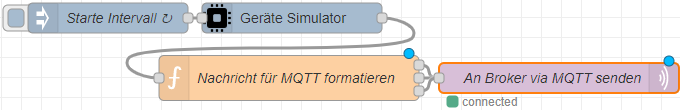
\includegraphics[width=\textwidth]{graphics/Device-Simulator-Flow.png}
\caption{Node-Red Flow des Sensorsimulators}
\label{abb:DeviceSimFlow}
\end{figure}

In \autoref{abb:DeviceSimFlow} ist ein Screenshot des Node-RED Flows zu sehen, in dem die verschiedenen Knoten, die jeweils eigene Aufgaben übernehmen, gezeigt sind. Da der Gerätesimulator die Nachrichten falsch formattiert übergibt, ist es notwendig, eigene Logik zur Reformattierung für den Transfer mit \ac{MQTT} einzusetzen. Diese ist mit einem $f$ gekennzeichnet.













\addtocontents{toc}{\protect\newpage}
\chapter{Dienstauswahl}
Im nachfolgenden Kapitel werden mittels der in \autoref{chap:vergleichsmethodik} vorgestellten Methodik die Dienste für die finalen Referenzarchitekturen unter den in \autoref{chap:rahmendatenverarbeitung} vorgestellten Rahmenbedingungen verglichen und ausgewählt.

\section{Angewandte Methodik}

Grundlage der hier gezeigten Bewertungskriterien sind die in \autoref{chap:vergleichsmethodik} gezeigten Kriterien von \citeauthor{Marz.2015}, die ISO 9126 Norm, die im Interview in \anhangref{anhang:interview-ralph-24.03.2021} eingebracht wurde und das Kriterium \enquote{serverlessness}, welches nicht die volle Punktzahl erreichen kann, wenn Skalierungsoperationen nicht automatisch durchgeführt werden können. Bei den Kriterien von \citeauthor{Marz.2015} wurde Ad hoc queries gestrichen, da manche Dienste nur zeitlich vorgeplante Auswertungen durchführen können, oder die Fähigkeit außerhalb des eigenen Ausführungsplans Anfragen zu bearbeiten, nicht besitzen. Ebenfalls wurde die Nachverfolgbarkeit als Kriterium ausgenommen, da ein geringer Wartungsaufwand im Wartungsfall diese bedingt. Die Performancegarantien werden genau wie die Kosten, welche ein eigenes Kriterium sind, nach eigener, in \autoref{chap:vergleichsmethodik} beschriebener Methodik evaluiert. Aus diesem Grund wurde \enquote{Lese- und Schreibzugriffe mit niedriger Latenz} in Performancegarantien umbenannt. Ausgehend von dieser Prioritätenliste wurde eine Umfrage zur Priorisierung durchgeführt, welche die finalen Prioritätengewichte, wie in \autoref{tab:umfragen-auswertungen} gezeigt, ergibt. 

\begin{table}[H]
\centering
\begin{tabular}{|l|l|l|}
\hline
Kriterium & \begin{tabular}[c]{@{}l@{}}Durchschnitt\\ ($n=6$)\end{tabular} & \begin{tabular}[c]{@{}l@{}}finale\\ Prioritäten\end{tabular} \\ \hline
Übertragbarkeit zwischen Clouds (ISO 9126) & 1,00 & 1 \\ \hline
Integration mit AWS & 3,17 &  3\\ \hline
Generalisierung & 4,33 &  4\\ \hline
Erweiterbarkeit & 4,33 &  4\\ \hline
Fehlertransparenz / \enquote{Debuggability} & 4,67 &  5\\ \hline
geringer Wartungsaufwand & 6,5 &  7\\ \hline
Skalierbarkeit  \& \enquote{serverlessness} & 7,17 &  7\\ \hline
Kosten & 7,33 &  7\\ \hline
Performancegarantien & 8,0 &  8\\ \hline
Robustheit \& Fehlertoleranz & 8,83 &  9\\ \hline
unterstützt Auswertungen (\autoref{chap:auswertungsarten}) & 10,67 & 11 \\ \hlinewd{2pt}
\rowcolor[HTML]{ECF4FF}
Summe & & 66\\ \hline
\end{tabular}
\caption{Auswertungen der Umfragen}
\label{tab:umfragen-auswertungen}
\end{table}

Die Ergebnisse der Umfrage sind in \autoref{tab:umfragen-auswertungen} dargestellt. Die Beschreibung des Vorgehens zur Umfrage ist in \anhangref{anhang:umfrage}. Insgesamt sind die Kriterien nach Priorität absteigend geordnet, welche gleichzeitig die Summe an Punkten darstellt, die maximal für dieses Kriterium zulässig sind.

Ausgehend von der Gesamtsumme der Punkte kann eine Rangliste erstellt werden, welche Dienstleistungen für die Referenzarchitektur verwendet werden können.



\section{Dienste für Echtzeitverarbeitung}\label{produkte:echtzeit}

In \autoref{abb:ProdukteRT} werden verwendbare Dienste von \ac{AWS}, gemeinsam mit ihren jeweiligen Einsatzgebieten gezeigt. In diesem Abschnitt soll besonders auf die Dienste zum Datenstreaming und zur Datenverarbeitung eingegangen werden. Gezeigt werden jedoch auch Dienste für -Speicherung, -Visualisierung und Machine Learning, da diese komplementär oder mit den prozessierten Daten verwendet werden können.
\begin{figure}[H]
\centering
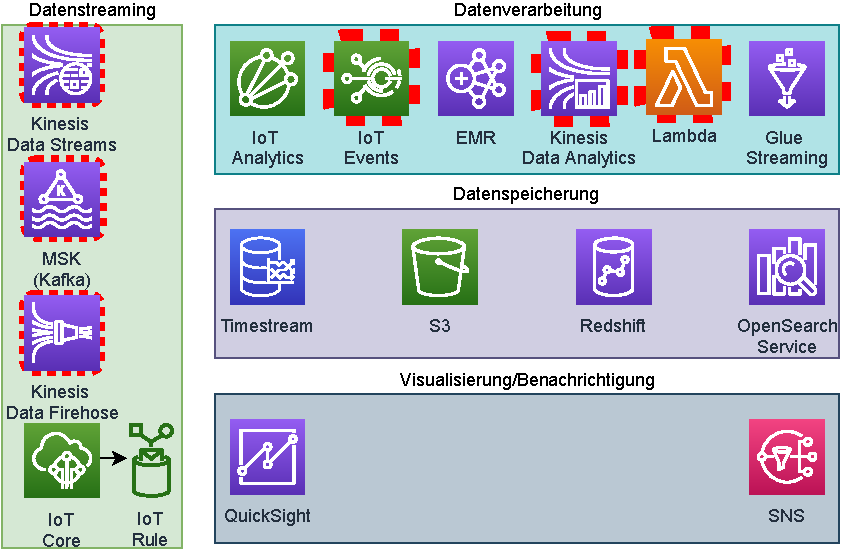
\includegraphics[width=\textwidth]{graphics/Overview-Realtime.pdf}
\caption{Einsetzbare Produkte im Bereich Echtzeitverarbeitung}
\label{abb:ProdukteRT}
\end{figure}


Innerhalb des \ac{IoT} Core Brokers ist es möglich, Regeln zu definieren, die einzelne Nachrichten aus Topics in andere Dienste weiterzuleiten. Dazu müssen besagte Nachrichten selektiert werden, was mittels eines SQL Dialekts möglich ist. Eine beispielhafte Selektion könnte folgendermaßen aussehen: 


\begin{figure}[H]
\centering
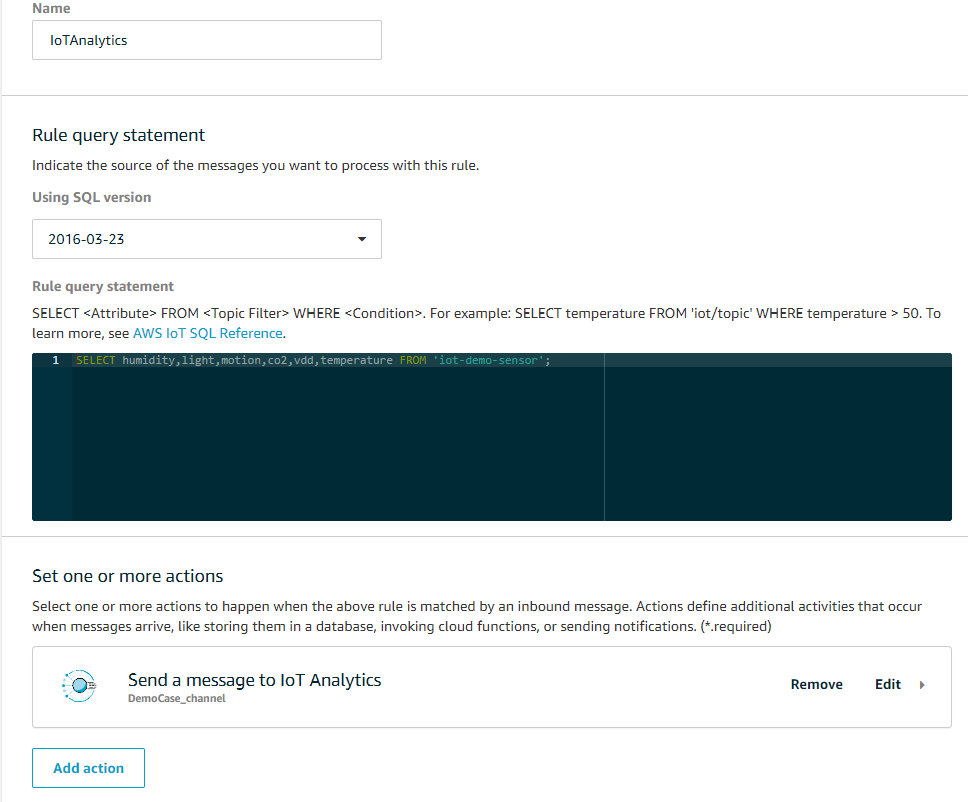
\includegraphics[width=\textwidth]{graphics/IoT-Rules-console.png}
\caption{Einstellung einer neuen Regel zur Weiterleitung an IoT Analytics}
\label{abb:IoTRulesExample}
\end{figure}

In \autoref{abb:IoTRulesExample} ist die Erstellung einer Weiterleitungsregel mit folgendem SQL Code zu sehen:
\begin{listing}[H]
\inputminted[frame=lines,breaklines=true]{sql}{code/iot-rules-example.sql}
\caption{IoT Rule Beispiel}
\label{listing:iot-rule-example}
\end{listing}
Die Nachrichten aus dem Topic iot-demo-sensor werden dabei beispielhaft an IoT Analytics weitergeleitet.

\begin{table}[H]
\centering
\begin{tabular}{|l|l|l|}
\hline
\rowcolor[HTML]{ECF4FF} 
Begründung & Kriterium & Bewertung \\ \hline
Einsatz von Code & Robustness and fault tolerance & 8 \\ \hline
Einsatz von Code, statische Analyse & Ad hoc queries & 0 \\ \hline
Anzahl der AWS-Dienste\textless{}5 & Integration mit AWS & 1 \\ \hline
Anzahl der AWS-Dienste=0 & Integration mit AWS & 0 \\ \hline
AWS-properitär & Übertragbarkeit & 0 \\ \hline
\end{tabular}
\caption{Spezielle Einstufungen einzelner Produktbesonderheiten}
\label{tab:einstufungen}
\end{table}



\subsection{AWS IoT Events}
Im Rahmen der \AWSIOT Produktfamilie gibt es neben dem bereits angesprochenen \AWSIOT Analytics ebenfalls \AWSIOT Events.  
Der Dienst dient nach Angaben von Amazon der Konfiguration von \enquote{If-Then-Else} Regeln, mit denen Ereignisse (also Events) erkannt und verarbeitet werden sollen, indem Aktionen ausgelöst werden.\footcite[Vgl.][]{AmazonWebServicesInc..o.J.b} Die Abläufe können dabei, ähnlich wie bei Node-Red graphisch konfiguriert werden. 
\begin{figure}[H]
\centering
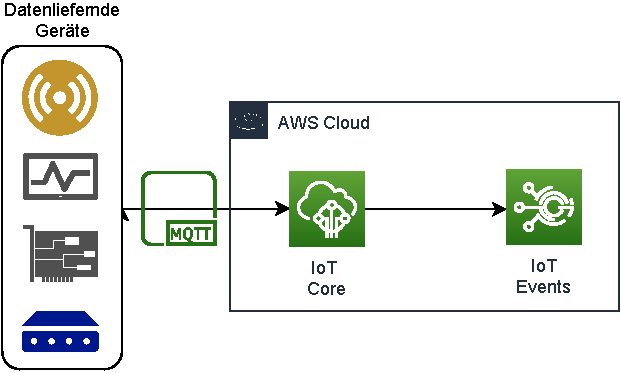
\includegraphics[width=0.8\textwidth]{graphics/IoT-Events-general.pdf}
\caption{Grobarchitektur des Ablaufes für IoT Events}
\label{abb:GrobArchitekturIoTEvents}
\end{figure}

\AWSIOT Events basiert auf abgebildeten Zuständen, die basierend auf ihren Übergängen Aktionen auslösen. \autoref{abb:BeispielIoTEvents} zeigt 3 beispielhaft 3 definierte Zustandsübergänge in der Weboberfläche von \AWSIOT Events. Jeder Kreis, welcher einen Zustand simbolisiert, hat 3 eigene Ereignisse, nämlich OnEnter, OnInput und OnExit. Zusätzlich sind Zustände mit Zustandsübergangspfeilen verbunden, welche basierend auf einer Ausführungskondition ausgelöst werden. Eine solche Ausführungskondition (auch Trigger genannt) wäre beispielsweise
\begin{lstlisting}
$input.Input1.value > $variable.threshold
\end{lstlisting}
\begin{figure}[H]
\centering
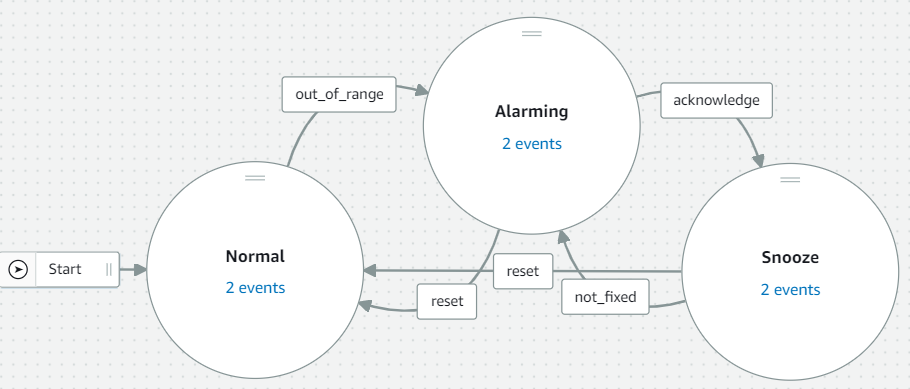
\includegraphics[width=\textwidth]{graphics/IoT-Events-Demo.png}
\caption{Beispiel IoT Events}
\label{abb:BeispielIoTEvents}
\end{figure}
Sollte ein Alarmzustand erreicht werden, können andere Dienste wie Lambda oder \ac{SNS} zur Verarbeitung oder Benachrichtigung integriert werden.

\produktbewertung{AWS~IoT~Events}{9,10,9,8,7,3,5,0,0,1,0,47}

\begin{table}[H]
\centering
\begin{tabular}{|l|l|l|}
\hline
Dimension & Preis(\$)/Einheit & Summe (\$) \\ \hline
evaluierte Regeln & \begin{tabular}[c]{@{}l@{}}0,000018/Regel\\ (teuerster Preis - ohne Volumenrabatt)\end{tabular} & 155,52 \\ \hline
Alarme & \begin{tabular}[c]{@{}l@{}}0,1/Alarm\\ (pro Sensor)\end{tabular} & 20 \\ \hline
\ac{SNS} (Push) & \begin{tabular}[c]{@{}l@{}}0,00002/Nachricht\\ (angenommen 5 Alarme/Gerät/Monat)\end{tabular} & 0,02 \\ \hline
Lambda Ausführungen & \begin{tabular}[c]{@{}l@{}}0,0000002/Ausführung\\ 0,0000000167/GB-Sekunde\end{tabular} & 0,08 \\ \hline
\begin{tabular}[c]{@{}l@{}}\ac{S3}-Speicher \\ (Lambda)\end{tabular} & 0,0245/GB Speicher & 0,0245 \\ \hline
Summe &  & \underline{175,6445} \\ \hline
\end{tabular}
\caption{Kostenvergleich AWS~IoT~Events}
\label{tab:kostenvergleich-AWS~IoT~Events}
\end{table}
Die Preise sind der offiziellen Preisaufstellung von \ac{AWS} entnommen. \footcite[Vgl.][]{AmazonWebServicesInc..o.J.k}

\subsection{Amazon Kinesis}
Amazon Kinesis ist im Gegensatz zu \AWSIOT Analytics nicht allein auf die Analyse von \ac{IoT} Daten spezialisiert. Kinesis eignet sich vielmehr für generelle Analysen von allerlei Streamingdaten. Zusätzlich ist Amazon Kinesis älter als \AWSIOT Analytics und bildet die technische Grundlage für die Verarbeitung \AWSIOT Events.\footcite[Vgl.][]{Pogosova.28.05.2020} Kinesis garantiert zusätzlich, dass Daten in 70 Milisekunden verfügbar sind.

Alternativ zur Kinesis Familie gibt es auch Open-Source Stream Analytics Produkte, wie von \citeauthor{Singh.2016} dargestellt.\footcite[Vgl.][]{Singh.2016} Diese kommen aufgrund der fehlenden Integration mit \ac{AWS} und des erhöhten Aufwands durch Eigenbetrieb nicht in Frage.

\begin{figure}[H]
\centering
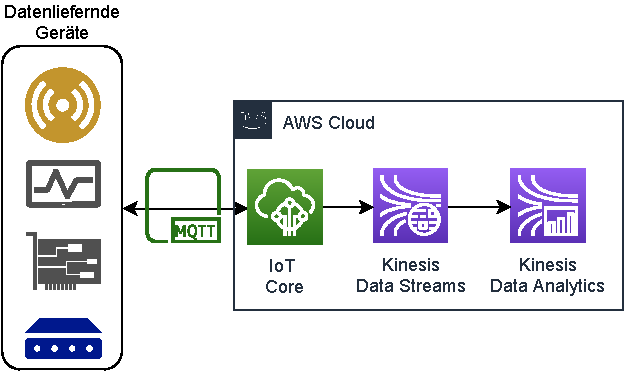
\includegraphics[width=0.8\textwidth]{graphics/Kinesis-Analytics-general.pdf}
\caption{Grobarchitektur des Ablaufes für Kinesis Analytics}
\label{abb:GrobArchitekturKinesisAnalytics}
\end{figure}
In \autoref{abb:GrobArchitekturKinesisAnalytics} ist das Zusammenspiel der Dienste aus der Kinesis Familie mit anderen Diensten dargestellt. Angenommen werden dabei die in \autoref{chap:rahmendatenverarbeitung} erläuterten Rahmenbedingungen, weshalb \ac{IoT} Core als Message Broker eingesetzt ist. Wie in der in \autoref{productselection:iotanalytics} beschriebenen Architektur, muss auch hier für die Datenverarbeitung eine Regel im \ac{IoT} Core Broker angelegt werden, um relevante Nachrichten an Kinesis Data Streams weiterzuleiten.\footcite[Vgl.][]{AmazonWebServicesInc..o.J.} Die tatsächliche Analyse übernimmt das komplementäre Produkt Kinesis Data Analytics.

\begin{figure}[H]
\centering
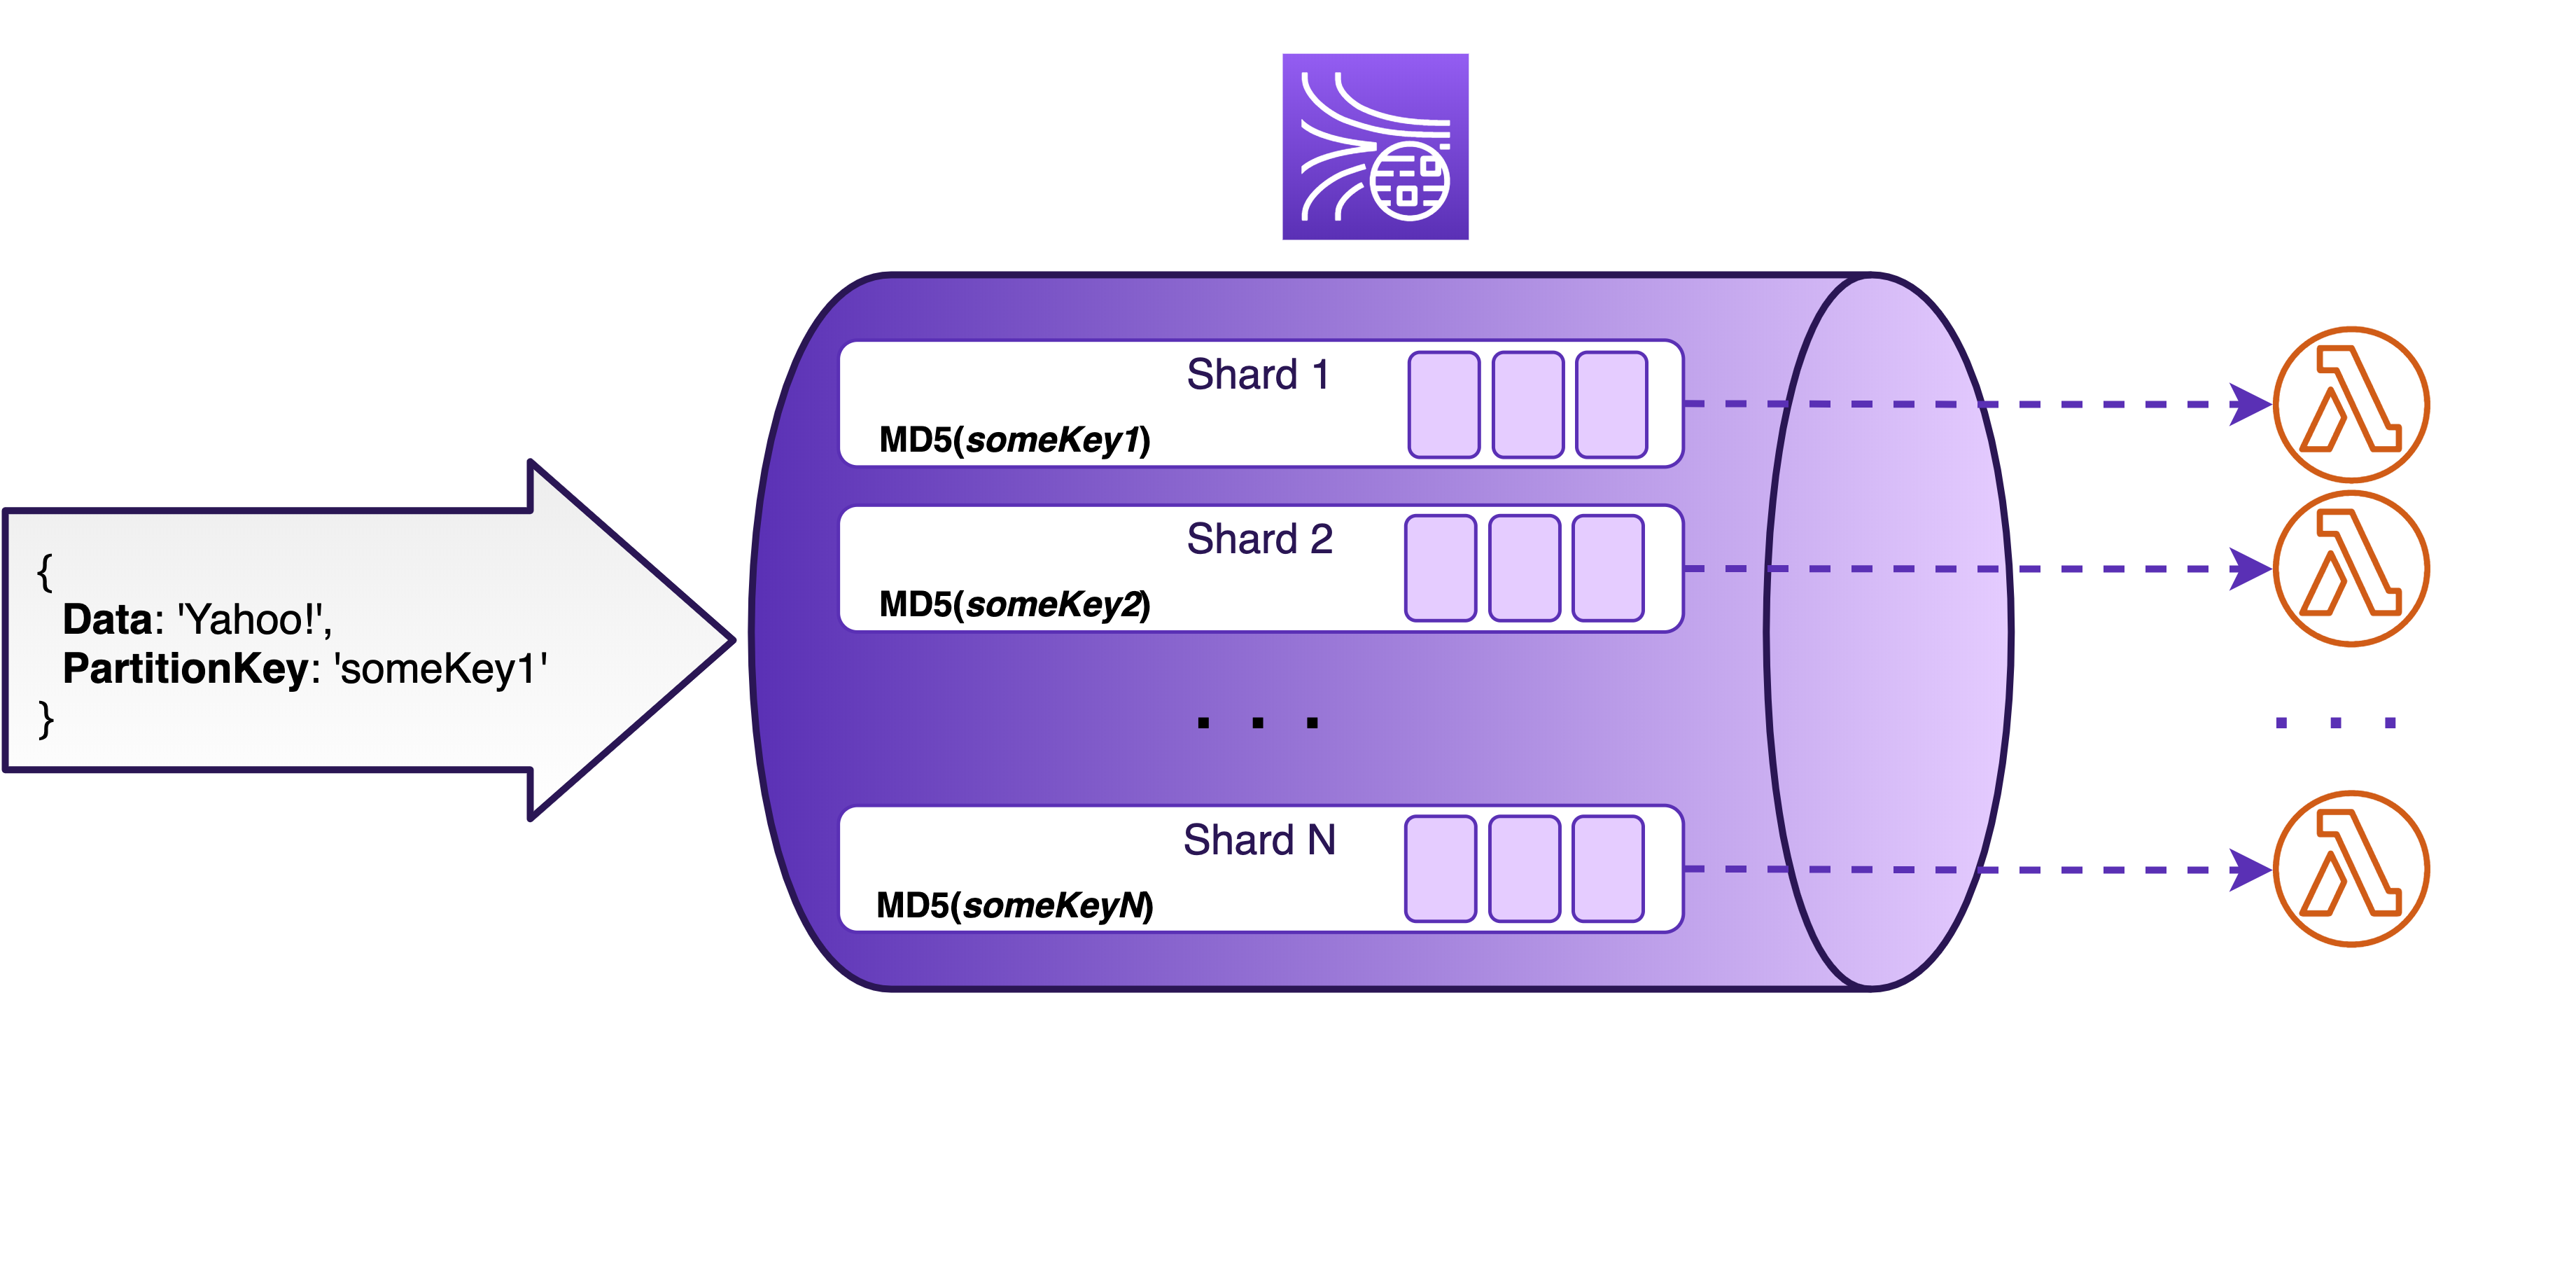
\includegraphics[width=\textwidth]{graphics/kinesis-inner-workings.png}
\caption[Funktionsweise von Kinesis]{Funktionsweise von Kinesis.\footnotemark}
\label{abb:KinesisShards}
\end{figure}
\footnotetext{Entnommen aus: \cite{Pogosova.28.05.2020}}
Kinesis Data Streams unterteilt, wie in \autoref{abb:KinesisShards} gezeigt, Daten in einzelne Partitionen/Shards, in denen gleich partitionierte Datensätze verarbeitet werden können.\footcite[Vgl. auch im Folgenden][]{Pogosova.28.05.2020} Einzelne Shards verhalten sich dabei wie geordnete Warteschlangen und speichern die Nachrichten nach Eingangsdatum sortiert. 

\produktbewertung{Amazon~Kinesis}{11,5,4,4,6,6,5,0,3,2,0,46}


\begin{table}[H]
\centering
\begin{tabular}{|l|l|l|}
\hline
Dimension & Preis(\$)/Einheit & Summe (\$) \\ \hline
\begin{tabular}[c]{@{}l@{}}Kinesis Data Streams\\ Shard-Stunde\end{tabular} & 0,018/h & 13,14 \\ \hline
\begin{tabular}[c]{@{}l@{}}Kinesis Data Streams\\ PUT-Operationen\end{tabular} & 0,0175/Million & 0,15 \\ \hline
\begin{tabular}[c]{@{}l@{}}Kinesis Data Analytics\\ Processing Unit\end{tabular} & 0,132/h & 32,12 \\ \hline
\ac{SNS} (Push) & \begin{tabular}[c]{@{}l@{}}0,00002/Nachricht\\ (angenommen 5 Alarme/Gerät/Monat)\end{tabular} & \textless{}0,02 \\ \hline
Lambda Ausführungen & \begin{tabular}[c]{@{}l@{}}0,0000002/Ausführung\\ 0,0000166667/Sekunde (angenommen: 5)\\ 0,0000000167/GB \acs{RAM}/ms\end{tabular} & 0,08 \\ \hline
Summe &  & \underline{45,51} \\ \hline
\end{tabular}
\caption{Kostenvergleich Amazon~Kinesis}
\label{tab:kostenvergleich-Amazon~Kinesis}
\end{table}

Siehe \footcite[][]{AmazonWebServicesInc..o.J.l}\nzitat\footcite[AmazonWebServicesInc..o.J.m][]{}\nzitat\footcite[Vgl.][]{AmazonWebServicesInc..2017b}



\subsection{AWS Lambda}
Bei \ac{AWS} Lambda handelt es sich um die Amazon Implementierung eines \ac{FaaS} Dienstes. Innerhalb dieser Arbeit wird Lambda als einzige generelle Computing Plattform betrachtet, da Alternativen wie \ac{EC2}, welches virtuelle Maschinen anbietet oder \ac{ECS}, welches Container anbietet einen von einzelnen Events unabhängigen Lebenszyklus haben. So laufen Container auf \ac{ECS} oder virtuelle Maschinen auf \ac{EC2}, wenn nicht anders konfiguriert kontinuierlich und holen/ \enquote{fetchen} Daten. In Zeiträumen, in denen keine Daten bereitstehen sind die entsprechenden Container und virtuellen Maschinen im Leerlauf, was unnötige Kosten erzeugt. Lambda hingegen wird von unterstützenden Diensten zur Verarbeitung von Events aufgerufen. Dabei ist je nach Dienst einstellbar, ob ein Aufruf pro Event stattfinden soll, oder Events zu einer konfigurierbaren Anzahl gruppiert werden und dann an Lambda übergeben werden. Lambda eignet sich besonders für analytische Workloads, seit der kürzlichen Addition von Intels \ac{AVX2}, einem speziellen CPU-Instruktionssatz, der die Verarbeitung von Vektorinstruktionen, wie sie beispielsweise beim Machine Learning oder in der Statistik vorkommen, beschleunigt.\footcite[Vgl.][]{Beswick.24.11.2020} Aufgrund der zentralen Rolle im Bereich Compute bei \ac{AWS}, können viele Dienste Events an Lambda senden. In \autoref{abb:GrobArchitekturLambda} sind als Integrationsbeispiele die \acp{MoM} \ac{IoT} Core, MQ und Kinesis Data Streams als Eventlieferanten gezeigt.
\begin{figure}[H]
\centering
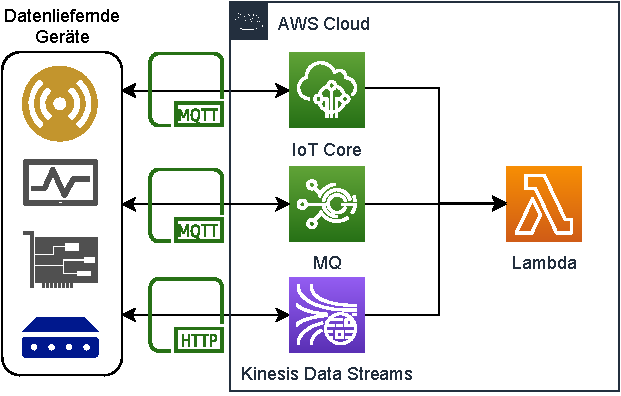
\includegraphics[width=0.8\textwidth]{graphics/Lambda-general.pdf}
\caption{Grobarchitektur des Ablaufes für Lambda}
\label{abb:GrobArchitekturLambda}
\end{figure}

\produktbewertung{AWS~Lambda}{8,10,9,6,7,6,0,0,3,2,1,52}

\begin{table}[H]
\centering
\begin{tabular}{|l|l|l|}
\hline
Dimension & Preis(\$)/Einheit & Summe (\$) \\ \hline
Lambda Ausführungen & 0,0000002/Ausführung & 1,728 \\ \hline
Lambda \textbackslash{}ac\{RAM\} & 0,0000000167 \#/GB-Sekunde & 720 \\ \hline
\ac{S3}-Speicher & 0,0245/GB Speicher & 0,0006 \\ \hline
Summe &  & \underline{721,73} \\ \hline
\end{tabular}
\caption{Kostenvergleich AWS~Lambda~Maximal}
\label{tab:kostenvergleich-AWS~Lambda~Maximal}
\end{table}

\autoref{tab:kostenvergleich-AWS~Lambda~Maximal} zeigt die möglichen Kosten, wenn für jede eingehende Nachricht eine Lambdafunktion aufgerufen und ausgeführt wird (unabhängig davon, dass das mit den Standardeinstellungen für Parallelität nicht realisierbar wäre). Um diese hohen Kosten zu mitigieren, gibt es mehrere Varianten. Folgend wird auf die Zwischenschaltung einer \ac{MOM}, nämlich \ac{AWS} \ac{SQS} und auf die Vorfilterung der Nachrichten durch \AWSIOT{} Core Rules näher eingegangen.

\autoref{abb:Lambda-Batch} zeigt die Zwischenschaltung von \ac{SQS} als Puffer, von dem asynchron gelesen werden kann.

\begin{figure}[H]
\centering
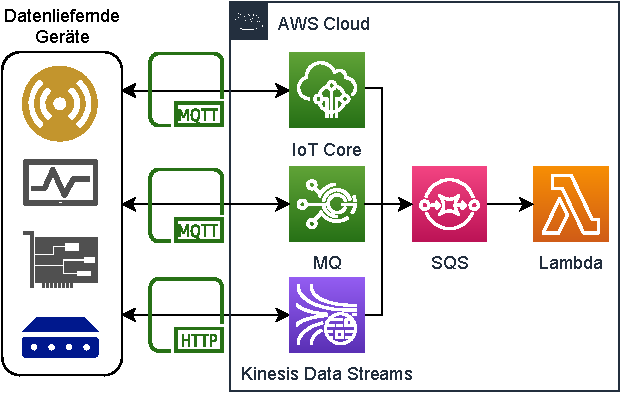
\includegraphics[width=0.8\textwidth]{graphics/Lambda-Batch.pdf}
\caption{Lambda Sammelverarbeitung via SQS}
\label{abb:Lambda-Batch}
\end{figure}

Seit November 2020 ist es in Lambda möglich, mittels der Einstellung \enquote{MaximumBatchingWindowInSeconds} das Übertragungsfenster frei zu definieren, in welchem auf Nachrichten von \ac{SQS} gewartet wird.\footcite[Vgl. auch im Folgenden][]{AmazonWebServicesInc..2020b} Dies erlaubt innerhalb eines maximalen Fensters von fünf Minuten Nachrichten zu sammeln und an Lambda zu übermitteln. Dies reduziert entsprechend die Ausführungen auf 20 pro Stunde und ist, wie in \autoref{tab:kostenvergleich-AWS~Lambda~Sammelverarbeitung} zu sehen, wesentlich günstiger.

\begin{table}[H]
\centering
\begin{tabular}{|l|l|l|}
\hline
Dimension & Preis(\$)/Einheit & Summe (\$) \\ \hline
Lambda Ausführungen & 0,0000002/Ausführung & 0,00288 \\ \hline
Lambda \ac{RAM} & 0,0000000167/GB-Sekunde & 1,2 \\ \hline
\ac{S3}-Speicher & 0,0245/GB Speicher & 0,0006 \\ \hline
\ac{SQS}-Durchsatz & 0,40/Million Anfragen & 3,456 \\\hline
Summe &  & \underline{4,65948} \\ \hline
\end{tabular}
\caption{Kostenvergleich AWS~Lambda~Sammelverarbeitung}
\label{tab:kostenvergleich-AWS~Lambda~Sammelverarbeitung}
\end{table}


Alternativ ist mittels einer angepassten Regel in \AWSIOT{} Rules, die in \autoref{listing:iot-rule-threshold} gezeigt ist, eine Ausführung nur bei Überschreitung des Schwellwerts möglich.

\begin{listing}[H]
\inputminted[frame=lines,breaklines=true]{sql}{code/iot-rules-lambda-filter.sql}
\caption{IoT Rule Schwellwertregel}
\label{listing:iot-rule-threshold}
\end{listing}
Diese Regel reduziert die rechnerischen Ausführungen auf 1000 pro Monat. Wie in \autoref{tab:kostenvergleich-AWS~Lambda~IOT~Sammelverarbeitung} gezeigt, fallen die Kosten bei 1000 Ausführung noch geringer als bei der gepufferten Variante mit \ac{SQS} aus. Es ist abhängig, ob eine Schwellwertüberprüfung in \AWSIOT{} Rules, speziell unter dem Paradigma der \enquote{Immutable Infrastructure}, welche unveränderliche, versionsverwaltete Infrastruktur fordert, als akzeptabel angesehen wird.\footcite[Vgl.][]{AmazonWebServicesInc..o.J.p} Für Änderungen an Schwellwerten müsste nämlich entsprechend die \AWSIOT{} Rule angepasst werden, was im \ac{SQS} durch eine einfach einzuspielende Codeänderung machbar wäre.

\begin{table}[H]
\centering
\begin{tabular}{|l|l|l|}
\hline
Dimension & Preis(\$)/Einheit & Summe (\$) \\ \hline
Lambda Ausführungen & 0,0000002/Ausführung & 0,0002 \\ \hline
Lambda \ac{RAM} & 0,0000000167/GB-Sekunde & 0,0833335 \\ \hline
\ac{S3}-Speicher & 0,0245/GB Speicher & 0,0006 \\ \hline
Summe &  & \underline{0,0841335} \\ \hline
\end{tabular}
\caption{Kostenvergleich AWS~Lambda~IOT~Sammelverarbeitung}
\label{tab:kostenvergleich-AWS~Lambda~IOT~Sammelverarbeitung}
\end{table}

\subsection{Amazon MSK}
Bei \ac{MSK} handelt es sich um einen Managed Service für die Open Source Lösung Apache Kafka. Im Gegensatz zu anderen, hier im Kapitel aufgeführten Lösungen wie \ac{IoT} Analytics, hat Amazon \ac{MSK} nicht von Grund auf selber entwickelt, sondern einen großen Teil des Codes von Apache Kafka übernommen. Dies erklärt auch, warum die Anbindung an andere Dienste von Amazon bedeutend schwieriger ist, als beispielsweise an \ac{IoT} Core. In der in \autoref{abb:GrobArchitekturMSK} abgebildeten Grobarchitektur müsste zur Anbindung von Apache Kafka an zuliefernde Geräte ein Intermediär wie \ac{IoT} Core verrwendet werden, da Apache Kafka ein eigenes, binäres Protokoll hat, welches sonst in die Geräte implementiert werden müsste. \Todo{letzten Halbsatz belegen} Fraglich ist, ob sich eine Implementierung des Kafka Protokolls auf allen Endgeräten lohnt, speziell im Licht besser unterstützter Standards wie \ac{MQTT}. Umgangen werden kann die Implementierung des Kafka Protokolls auf zuliefernden Geräten auf dreierlei Arten: Zum einen lassen sich mittels Kafka Connect for \ac{MQTT} \ac{MQTT} Broker als Eventquellen anbinden.\footcite[Vgl.][]{Erber.12.01.2021} Alternativ kann Kafka auch als \ac{MQTT} Proxy dienen, was bedeutet, dass Kafka als eigenständiger MQTT Broker agiert, wobei zu beachten ist, dass Kafka weit nicht alle \ac{MQTT} Standardelemente implementiert und eine paralelle Weiterverarbeitung in anderen Amazon Diensten nicht möglich ist.\footcite[Vgl.][]{Erber.12.01.2021} Zuletzt gibt es noch die Möglichkeiten, die Nachrichten via \ac{IoT} Core innerhalb von \ac{AWS} an \ac{MSK} weiterzuleiten, was auch in \autoref{abb:GrobArchitekturMSK} dargestellt ist.
\begin{figure}[H]
\centering
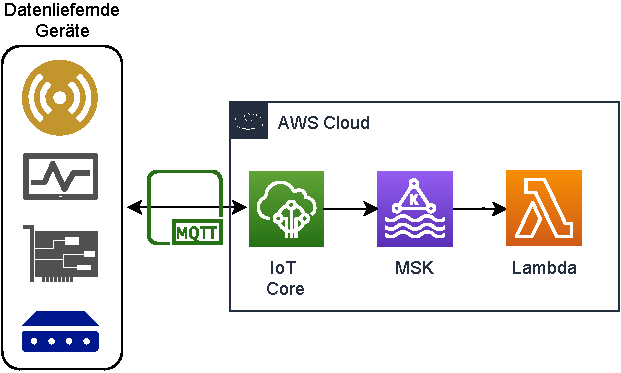
\includegraphics[width=0.8\textwidth]{graphics/MSK-general.pdf}
\caption{Grobarchitektur des Ablaufes für Managed Streaming for Apache Kafka}
\label{abb:GrobArchitekturMSK}
\end{figure}

Kafka hat eigene Verarbeitungslogiken integriert, mit welchen einige Analysen bereits durchgeführt werden können. Um diese in \ac{AWS} weiterverarbeiten zu können, müssen die Ergebnisse via der Integration mit Lambda oder der Integration mit \ac{EC2}, der Amazon Plattform für virtuelle Maschinen abgerufen werden.

\produktbewertung{Amazon~MSK}{11,5,4,7,5,6,5,0,3,1,1,48}



\begin{figure}[H]
\centering
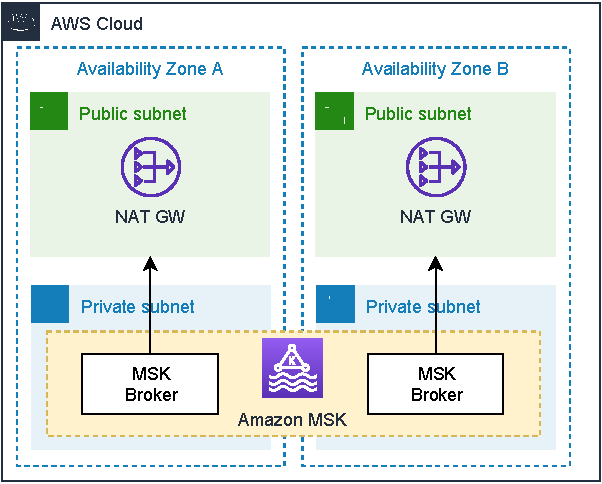
\includegraphics[width=0.55\textwidth]{graphics/MSK-Networking.pdf}
\caption[Networking MSK]{Networking MSK.\footnotemark}
\label{abb:NetworkingMSK}
\end{figure}
\footnotetext{Mit Änderungen entnommen aus: \cite{Beswick.2020}}

\begin{table}[H]
\centering
\begin{tabular}{|l|l|l|}
\hline
Dimension & Preis(\$)/Einheit & Summe (\$) \\ \hline
\begin{tabular}[c]{@{}l@{}}Broker Instanz\\ (t3.small - 2 mal)\end{tabular} & 0,0526/h & 76,7960 \\ \hline
Broker Storage & 0,119/h & 0,714 \\ \hline
\begin{tabular}[c]{@{}l@{}}NAT Gateway\\ (2 mal)\end{tabular} & \begin{tabular}[c]{@{}l@{}}0,052/h\\ 0,052/GB\end{tabular} & 76,34 \\ \hline
Lambda Ausführungen & 0,0000002/Ausführung & 0,00288 \\ \hline
Lambda \ac{RAM} & 0,0000000167/GB-Sekunde & 1,2 \\ \hline
\ac{S3}-Speicher & 0,0245/GB Speicher & 0,0006 \\ \hline
Summe &  & \underline{155,05348} \\ \hline
\end{tabular}
\caption{Kostenvergleich Amazon~MSK}
\label{tab:kostenvergleich-Amazon~MSK}
\end{table}

Lambda: Maximal 10.000 Events

\footcite[Vgl.][]{AmazonWebServicesInc..o.J.o}\nzitat\footcite[Vgl.][]{Beswick.2020}

% => binary protocol no \ac{MQTT} Support, redundant, only Lambda and EC2 conenctivity

\subsection{AWS Glue}
Mittels dem \ac{AWS} Glue Dienst, welcher diverse \ac{ETL} Dienste, wie beispielsweise Datenkatalogisierung und Datentransformation basierend auf dem Apache Spark Ökosystem anbietet, können ebenfalls Streams analysiert werden.\footcite[Vgl.][]{AmazonWebServicesInc..o.J.d}\nzitat\footcite[Vgl. auch im Folgenden][]{AmazonWebServicesInc..2020} Basierend auf der Apache Spark Structured 
Streaming-Engine können nach Aussage des Herstellers Daten aus Kinesis oder Kafka (und damit aus \ac{MSK}) geladen werden. Nachfolgend werden die eingehenden Daten mittels sogenannter Jobs analysiert/transformiert, welche in Sprachen wie Scala, Java, Python oder R geschrieben sein können. Nach Abschluss der Analyse können die Daten in \ac{S3} oder in eine \ac{JDBC} kompatible Datenbank (z.B. MySQL, PostgreSQL, Amazon Redshift, Oracle Databse, ...) geladen werden.\footcite[Vgl.][]{AmazonWebServicesInc..o.J.e} Die Interaktion zwischen eigener Logik und AWS Glue erfolgt via \acp{API} von Apache Spark, die entsprechende Kentnisse zur Interaktion mit den Daten erfordern.

\produktbewertung{AWS~Glue}{8,10,9,6,4,4,5,0,2,1,0,49}

\begin{table}[H]
\centering
\begin{tabular}{|l|l|l|}
\hline
Dimension & Preis(\$)/Einheit & Summe (\$) \\ \hline
\begin{tabular}[c]{@{}l@{}}Broker Instanz\\ (t3.small - 2 mal)\end{tabular} & 0,0526/h & 76,7960 \\ \hline
Broker Storage & 0,119/h & 0,714 \\ \hline
\begin{tabular}[c]{@{}l@{}}NAT Gateway\\ (2 mal)\end{tabular} & \begin{tabular}[c]{@{}l@{}}0,052/h\\ 0,052/GB\end{tabular} & 76,34 \\ \hline
Lambda Ausführungen & 0,0000002/Ausführung & 0,00288 \\ \hline
Lambda \ac{RAM} & 0,0000000167/GB-Sekunde & 1,2 \\ \hline
\ac{S3}-Speicher & 0,0245/GB Speicher & 0,0006 \\ \hline
Summe &  & \underline{155,05348} \\ \hline
\end{tabular}
\caption{Kostenvergleich AWS~Glue}
\label{tab:kostenvergleich-AWS~Glue}
\end{table}

\subsection{Produktauswahl}

\begin{table}[H]
\centering
\begin{tabular}{|l|l|l|}
\hline
Platz & Name & Summe \\ \hline
1 & AWS Lambda & \cellcolor[HTML]{DAE8FC}52 \\ \hline
2 & AWS Glue & \cellcolor[HTML]{DAE8FC}49 \\ \hline
3 & Amazon MSK & \cellcolor[HTML]{DAE8FC}48 \\ \hline
4 & AWS IoT Events & \cellcolor[HTML]{DAE8FC}47 \\ \hline
5 & Amazon Kinesis & \cellcolor[HTML]{DAE8FC}46 \\ \hline
\end{tabular}
\caption{Produktreihenfolge Echtzeitprodukte}
\label{tab:Reihenfolge-Echtzeit}
\end{table}


\section{Dienste für Batchverarbeitung}

In \autoref{abb:ProdukteDB} werden verwendbare Dienste für die Batch (\enquote{\ac{OLAP}}) Verarbeitung von \ac{AWS}, gemeinsam mit ihren jeweiligen Einsatzgebieten gezeigt. In diesem Abschnitt soll besonders auf die Dienste zur Verarbeitung nach dem Laden der Daten in eine der gezeigten Datenquellen eingegangen werden. Gezeigt werden jedoch auch Dienste für Datenvisualisierung und Machine Learning, da diese komplementär oder mit den prozessierten Daten verwendet werden können. Da die einzelnen Datenquellen jeweils verschiedene Sprachen, bzw. Dialekte von \ac{SQL} verwenden, sind die spezifischen Abfragesprachen mit einem generischen Eintrag in der Grafik abgebildet. Dabei ist es bei \ac{AWS} durchaus üblich, Interoperabilität zu anderen \ac{AWS} Diensten, wie beispielsweise Lambda, in den jeweiligen \ac{SQL} Dialekt einzubauen.

\begin{figure}[H]
\centering
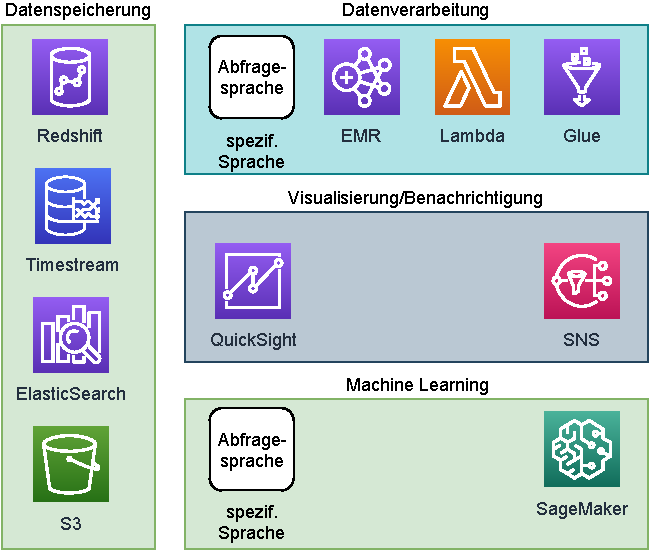
\includegraphics[width=\textwidth]{graphics/Overview-DB.pdf}
\caption{Einsetzbare Dienste im Bereich Datenbankverarbeitung}
\label{abb:ProdukteDB}
\end{figure}

\TodoW{brauchen wir das wirklich?}


\subsection{Amazon Timestream}
Timestream ist nach Aussage des Herstellers eine schneller, skalierbare und speziell für Zeitreihendaten entwickelte Datenbank, welche über \ac{AWS} als Dienstleistung bezogen werden kann.\footcite[Vgl. auch im Folgenden][]{AmazonWebServicesInc..o.J.h} Timestream integriert zwei verschiedene Speichertypen, nämlich \ac{RAM}-basierten Speicher, in dem Daten, auf welche schnell zugegriffen werden sollen, gespeichert werden können und Festplatten-basierten Speicher, welcher für historische Daten dienen soll.
Timestream besitzt zusätzlich einen eigenen \ac{SQL}-Dialekt, welcher um Funktionen zur Analyse von Zeitreihendaten erweitert wurde. 


% Ein Beispiel für den Einsatz des \ac{SQL}-Dialekts zur Abfrage der Informationen für den Anwendungsfall, der zum Kostenvergleich beschrieben wurde, ist in \autoref{listing:timestream-kostenvergleich} zu sehen.

% \begin{listing}[H]
% \inputminted[frame=lines,breaklines=true]{sql}{code/timestream-threshold.sql}
% \caption{Abfrage für Kostenvergleichs Usecase}
% \label{listing:timestream-kostenvergleich}
% \end{listing}

Timestream ist nicht selbst in der Lage, Abfragen zu planen. \ac{AWS} gibt in der Dokumentation an, dass Lambda verwendet werden kann, um periodisch eine Abfrage in Timestream auszuführen und basierend auf dieser Anfrage Alarme via \ac{SNS} zu versenden.\footcite[Vgl.][]{AmazonWebServicesInc..o.J.ag} Abgebildet ist diese Interaktion in \autoref{abb:TimestreamLAmbdaOrchestration}.


\begin{figure}[H]
\centering
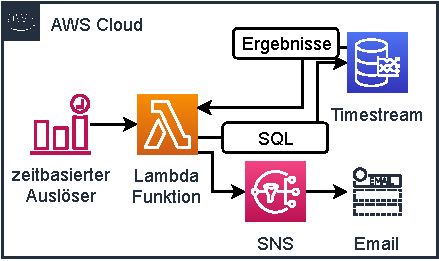
\includegraphics[width=0.45\textwidth]{graphics/Lambda-Timestream-Orchestration.pdf}
\caption{Orchestrierung von zeitbasierten Timestream Abfragen}
\label{abb:TimestreamLAmbdaOrchestration}
\end{figure}

\subsubsection{Features des Dienstes}
Perzentile lassen sich mit der eingebauten Funktion \mintinline{sql}{approx_percentile(x, percentage)} berechnen, der Mittelwert via \mintinline{sql}{avg(x)} oder \mintinline{sql}{geometric_mean(x)}
Eine native Anomalieerkennung bietet Timestream nicht, jedoch kann die Machine Learning Dienstleistung Amazon SageMaker Daten von Timestream analysieren und Anomalieerkennung ausführen.\footcite[Vgl. auch im Folgenden][]{AmazonWebServicesInc..o.J.aj} In SageMaker kann auch der nativ in Kinesis Data Analytics verbaute Random Cut Forest Algorithmus verwendet werden, um Anomalien zu erkennen. Andernfalls kann, wie von \citeauthor{Salgado.2019} beschrieben, eine einfache Anomalieerkennung durch Überprüfung des Wertes auf Lage zwischen dem 25. und 75. Quantil erfolgen.\footcite[Vgl.][]{Salgado.2019}
Die Schwellwertüberschreitungserkennung ist mittels einer einfachen \mintinline{sql}{WHERE} Bedingung machbar.
Ein gleitender Durchschnitt ist, wie von \citeauthor{Ross.2020} gezeigt, in SQL mittels der Bearbeitungsfenster, die Timestream, wie viele andere \ac{SQL} Implementierungen anbietet, möglich.\footcite[Vgl.][]{Ross.2020} Gleichzeitig unterstützt Amazon Timestream die Verwendung von Ableitungen als Werkzeug zur Trenderkennung.\footcite[Vgl.][]{AmazonWebServicesInc..o.J.ai}

\subsubsection{Performancegarantien}
Die \ac{SLA} von Timestream bietet allein 99,99\% Verfügbarkeit pro Verrechnungsmonat.\footcite[Vgl.][]{AmazonWebServicesInc..2020d} \ac{AWS} verspricht aber eine bis zu tausendfache Geschwindigkeitsverbesserung gegenüber relationalen Datenbanken.\footcite[Vgl.][]{AmazonWebServicesInc..o.J.ak}

Mitbewerber von \ac{AWS} im Bereich der Zeitseriendatenbanken haben in ihren Tests festgestellt, dass Timestream langsamer als ihre Konkurrenzdienste/Konkurrenzprodukte waren.\footcite[Vgl.][]{Booz.2020}\nzitat\footcite[Vgl.][]{Crate.ioInc..2020} Dabei sind die Testskripte von \citeauthor{Booz.2020} Open Source und damit die Messungen theoretisch reproduzierbar. Gleichzeitig gibt \ac{AWS} aber in einem Blogeintrag aus dem November an, Datensätze im Bereich von einem bis 21,7 TB analysieren zu können, ohne 100 Sekunden Ausführungszeit zu überschreiten.\footcite[Vgl.][]{Das.2020} Auch für diese Tests ist der Quellcode open source verfügbar.

Es kann keine finale Aussage über die genauen Performancegarantien getroffen werden, da entweder die Daten der Mitbewerber von \ac{AWS} als gültig anzunehmen sind, oder die Daten von \ac{AWS} selbst. Da es im kommerziellen Interesse aller Parteien liegt Timestream entweder auf- oder abzuwerten ist eine stichhaltige Aussage nicht möglich.

\subsubsection{Gesamtkosten}


Timestream ist momentan noch nicht in Frankfurt verfügbar, weshalb die Kosten in der einzigen europäischen Zone mit verfügbarem Timestream, Irland, als Maßstab verwendet werden. Angenommen wird, dass die Daten eine Stunde im \ac{RAM} vorgehalten werden und danach in die Festplattenspeicherung überführt werden.

%  Angenommen 8.640.000 (8,64 GB)/Monat 0,012GB/h 4,885056
% Abfrage: 25,92 GB

Ausgehend von dem beschriebenen Szenario lässt sich nicht genau errechnen, welche Datenmenge von den Anfragen genau erfasst wird. Dies ist dem Fakt geschuldet, dass Timestream die Daten optimiert abspeichert und nur den tatsächlichen Messwert speichert. Numerische Daten können als 32-bit int, als 64bit BigInt oder als 64bit double gespeichert werden.\footcite[Vgl. auch im Folgenden][]{AmazonWebServicesInc..o.J.r}\nzitat\footcite[Vgl. auch im Folgenden][]{AmazonWebServicesInc..o.J.q} Wenn dazu ein String für die Sensorid im Stile \enquote{Sensor-123} angenommen wird, der 19 bytes zur Darstellung benötigt und der Zeitstempel addiert wird, der 8 bytes benötigt, ergibt sich eine Speicherbelegung von 91 Bytes. Speicherkosten werden aber bei Werten unter einem Kilobyte auf einen Kilobyte hochgerundet, weshalb dies in der Speicherrechnung keine Beachtung findet. Wenn man weitere Optimierungen, die die Abfrageengine macht außer Acht lässt, muss mit 0,78624GB pro abgefragtem Monat gerechnet werden.


\begin{table}[H]
\centering
\begin{tabular}{|l|l|l|}
\hline
Dimension & Preis(\$)/Einheit & Summe (\$) \\ \hline
Schreibzugriffe & 0,5654/Mio./KB & 4,8851 \\ \hline
\begin{tabular}[c]{@{}l@{}}\ac{RAM} \\ Speicherung\end{tabular} & 0,0407/GB/h & 0,3516 \\ \hline
\begin{tabular}[c]{@{}l@{}}Festplatten\\ Speicherung\end{tabular} & 0,0339/GB/Monat & 0,8787 \\ \hline
Anfragen & \begin{tabular}[c]{@{}l@{}}0,011308/GB \\ abgefragt\end{tabular} & 25,6055 \\ \hline
Step Functions & \begin{tabular}[c]{@{}l@{}}0,025/1000 \\ Zustandsübergänge\end{tabular} &  1,08\\ \hline
Lambda Ausführungen & 0,0000002/Ausführung & 0,0002 \\ \hline
Lambda \ac{RAM} & 0,0000000167/GB-Sekunde & 0,08 \\ \hline
\ac{SNS} (Push) & \begin{tabular}[c]{@{}l@{}}0,00002/Nachricht\\ (angenommen 5 Alarme/Gerät/Monat)\end{tabular} & 0,02 \\ \hline
Summe & \cellcolor[HTML]{EFEFEF} & 32,9011 \\ \hline
\end{tabular}
\caption{Kostenvergleich AWS~Timestream}
\label{tab:kostenvergleich-AWS~Timestream}
\end{table}

\subsection{Amazon Athena/Amazon S3}\label{chap:athena}


Amazon Athena ist nach Aussage des Herstellers ein voll verwalteter Query Dienst, welcher das Durchsuchen von großen Datenmengen im \ac{S3} Speicherdienst möglich macht.\footcite[Vgl.][]{Barr.2016} Athena basiert dabei auf dem ursprünglich von Facebook entwickelten Presto, welches mittlerweile Open Source ist. Innerhalb von Athena können Daten verschiedener Formate (\ac{CSV}, Apache Parquet, Apache ORC, \ac{JSON}, ...) mittels \ac{SQL} verarbeitet werden. Zusätzlich ist seit November 2020 mittels der sogenannten \enquote{Federated Queries} auch die Abfrage von anderen Datenquellen wie Apache HBase, Amazon Document DB oder von Datenquellen, die durch eigenentwickelte Verbindungselemente verknüpft werden.\footcite[Vgl.][]{AmazonWebServicesInc..o.J.s} Technisch werden diese Federated Queries via Lambda abgewickelt.

Bei verändernden Datenschemata wird empfohlen, den Dienst \ac{AWS} Glue Crawler komplementär einzusetzen, welcher die Schemata aus \ac{S3} automatisch extrahiert und in Athena hinterlegt. Andernfalls können die Schemata auch manuell hinterlegt werden.

\begin{figure}[H]
\centering
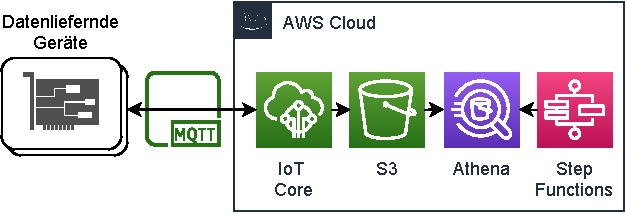
\includegraphics[width=0.8\textwidth]{graphics/Athena-general.pdf}
\caption{Grobarchitektur des Ablaufes für Athena}
\label{abb:GrobArchitekturAthena}
\end{figure}
\TodoW{In Text einbauen}

\subsubsection{Features des Dienstes}
Die technische Grundlage für Athena, ist das OpenSource Projekt Presto. Dieses bietet mit \mintinline{sql}{approx_percentile(x, percentage)} eine Funktion zur Kalkulation von Perzentilen an.\footcite[Vgl.][]{ThePrestoFoundation.o.J.}
Eine Möglichkeit, um Anomalien in Athena zu erkennen, ist es alle Werte, die ausserhalb der Spanne zwischen dem 25. und 75. Quantil liegen als Anomalie zu klassifizieren.\footcite[Vgl.][]{Salgado.2019} Dies wäre mit der \mintinline{sql}{approx_percentile(x, percentage)} Funktion von Athena machbar. Andernfalls könnte wie von \citeauthor{Megler.2016} vorgeschlagen, der Amazon \ac{EMR} Dienst benutzt werden, um Anomalien mittels der Bildung von Clustern und der Kalkulation der Distanz von Werten zu diesen Clustern zu detektieren.\footcite[Vgl.][]{Megler.2016}
Schwellwertüberschreitungen können via einer \mintinline{sql}{WHERE} Bedingung, wie bei Timestream auch, erkannt werden.
Wie bei Timestream auch kann nach der Methode von \citeauthor{Ross.2020} ein gleitender Durchschnitt mittels der Verarbeitungsfenster kalkuliert werden.\footcite[Vgl.][]{Ross.2020}

\subsubsection{Performancegarantien}

\citeauthor{Hartland.2018} beschreiben einen Anwendungsfall, in dem sie Athena zur Analyse von Logdaten innerhalb der Datenanalyseinfrastruktur des ATLAS Experiments am Large Hadron Collider im CERN Forschungszentrum bei Genf verwenden.\footcite[Vgl.][]{Hartland.2018}

Gleichzeitig stellen \citeauthor{Hartland.2018} auch fest, dass es Teil des Entwicklungsprozesses ist, die Anfragen zu  optimieren, um Kosten zu sparen.\footcite[Vgl.][5]{Hartland.2018} Dies entstammt der Natur von \ac{SQL} basierten Abfragemechanismen, da verschiedene Abfragestile und Operationen auf verschieden viele Speicherpartitionen zugreifen müssen. Da Athena nach Volumen der Speicherzugriffe abrechnet, kann es also sinnvoll sein, den Speicher nach Abfragearten zu partitionieren oder die Abfragen zu optimieren. Dazu können der im April 2021 vorgestellten \mintinline{sql}{EXPLAIN} \ac{SQL}-Befehl und die damit zusammenhängenden query execution plans verwendet werden.\footcite[Vgl. auch im Folgenden][]{AmazonWebServicesInc..2021} Diese zeigen nach Aussage von \ac{AWS} auf, wie eine Abfrage ausgeführt werden würde und wie Laufzeiten optimiert werden können.

Die reale Performance der bearbeiteten Anfragen garantiert \ac{AWS} nicht. Da Athena ein serverless Dienst ist, dessen unterliegende Kapazität vollständig von \ac{AWS} verwaltet wird, können Nutzende keinen Einfluss auf die provisionierten Ressourcen nehmen. Zusätzlich hängt die Performance stark von der Partitionierung der Daten und der Kompression ab.\footcite[Vgl.][]{Levy.2021} Zusätzlich zu beachten ist, dass Athena eine Limitierung von 20 (25 in der North Virginia Region) parallel laufenden/wartenden Anfragen hat und Anfragen nach 30 Minuten Laufzeit abgebrochen werden. \footcite[Vgl. auch im Folgenden][]{AmazonWebServicesInc..o.J.ac} Diese Limitierungen können jedoch auf Anfrage erhöht werden.

Amazon garantiert vertraglich keine Performance, sondern nur die 99,99\% Verfügbarkeit des Dienstes in dem \ac{SLA}.\footcite[Vgl.][]{AmazonWebServicesInc..2019c} In Vergleichen von \citeauthor{Levy.2019} und \citeauthor{Khadtare.2018} mit dem Mitbewerber Google BigQuery zeigte Athena schlechtere Performance, gemessen an den Antwortzeiten der Abfragen, war aber günstiger.\footcite[Vgl.][]{Levy.2019}\nzitat\footcite[Vgl.][]{Khadtare.2018} Da \ac{AWS} Ende 2020 mit Athena engine version 2 wesentliche Performanceverbesserungen angekündigt hat, ist nicht bekannt, ob die Daten noch aktuell sind.\footcite[Vgl.][]{AmazonWebServicesInc..2020c}

\subsubsection{Gesamtkosten}
Für die folgende Kostenbewertung wird angenommen, dass Athena die Daten aus \ac{S3} indiziert. Dort liegen die Daten im \ac{JSON} Format gespeichert vor. Zu beachten ist, dass effizientere Formate wie CSV, oder sogar Apache Parquet und ORC verfügbar sind. Diese können komprimiert Daten speichern. Eine Verwendung von Parquet oder ORC würde laut \ac{AWS} 30-90\% Kosten sparen.\footcite[Vgl.][]{AmazonWebServicesInc..o.J.t} Gleichzeitig kann aber eine Speicherung im \ac{JSON} Format via \AWSIOT{} Rule erfolgen, ohne dass weitere Verarbeitung notwendig ist.

% \begin{figure}[H]
% \centering
% 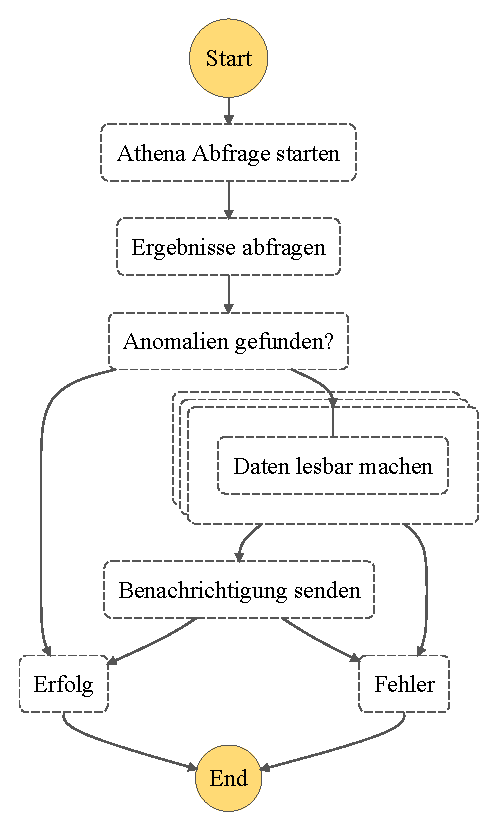
\includegraphics[height=0.45\textheight]{graphics/Step-Function-Athena.pdf}
% \caption{Beispiel Step Function State Machine}
% \label{abb:StepFunctionExample}
% \end{figure}
% \TodoW{Bild horizontal}

In \autoref{tab:kostenvergleich-Amazon~Athena} wird davon ausgegangen, dass 2MB an Daten im Zeitraum von 10 Minuten neu hinzukommen. Da aber eine Historie gebildet werden soll, müssen sowieso die gesamten dreimonatigen historischen Daten abgefragt werden. Ausgehend von 200 kB pro Minute von allen Geräten ergeben sich 25,92 GB Datenvolumen an historischen Daten, welche 960 mal im Monat abgefragt werden sollen. Athena rundet dabei auf das nächste MegaByte auf und hat ein Minimum von 10 MB erfasster Daten pro Anfrage.\footcite[Vgl.][]{AmazonWebServicesInc..o.J.t} Das Datenschema für Athena stellt Glue bereit, welches Kosten für Abfragen aus dem Datenkatalog und Speicherkosten für den Datenkatalog erhebt.\footcite[Vgl.][]{AmazonWebServicesInc..o.J.u} Zur Orchestrierung wird ein Ablauf als Zustandsmaschine in StepFunctions abgebildet, welches für jeden Zustandsübergang eine Gebühr erhebt.\footcite[Vgl.][]{AmazonWebServicesInc..o.J.v}

\begin{table}[H]
\centering
\begin{tabular}{|l|l|l|}
\hline
Dimension & Preis(\$)/Einheit & Summe (\$) \\ \hline
Athena Abfragen & \begin{tabular}[c]{@{}l@{}}0,005/TB \\ abgefragte Daten\end{tabular} &  121,50\\ \hline
\begin{tabular}[c]{@{}l@{}}Glue Data Catalog\\ Speicher\end{tabular} & 1/100.000 Objekte &  \textless 0,0001\\ \hline
\begin{tabular}[c]{@{}l@{}}Glue Data Catalog\\ Abfragen\end{tabular} & 1/Million Abfragen &  \textless 0,0001\\ \hline
Step Functions & \begin{tabular}[c]{@{}l@{}}0,025/1000 \\ Zustandsübergänge\end{tabular} &  1,08\\ \hline
\ac{SNS} (Push) & \begin{tabular}[c]{@{}l@{}}0,00002/Nachricht\\ (angenommen 5 Alarme/Gerät/Monat)\end{tabular} & 0,02 \\ \hline
Summe & \cellcolor[HTML]{EFEFEF} &  122,60\\ \hline
\end{tabular}
\caption{Kostenvergleich Amazon~Athena}
\label{tab:kostenvergleich-Amazon~Athena}
\end{table}



\subsection{Amazon Redshift}

Amazon Redshift ist der Data Warehouse Dienst von \ac{AWS}, welcher nach Aussage des Herstellers \enquote{enterprise-level} ist und auf ein Datenvolumen von Petabytes skalieren kann. \footcite[Vgl.][1]{AmazonWebServicesInc..o.J.g} Redshift ist dabei ein klassischer \ac{OLAP} Dienst, welcher für eine Vielzahl verschiedener Daten effizient Auswertungen bereitstellen kann. Redshift basiert auf der bekannten Open Source Datenbank PostgreSQL, weicht jedoch in der Implementierung diverser Kommandos und Features ab, die Amazon als irrelevant für \ac{OLAP} Anwendungen hält.\footcite[Vgl.][4]{AmazonWebServicesInc..o.J.g}\nzitat\footcite[Vgl.][428\psqq]{AmazonWebServicesInc..o.J.g} Kern von Redshift sind sogenannte Cluster, welche aus einer oder mehrerer Berechnungsknoten (\enquote{compute nodes}) und Anführerknoten (\enquote{leader nodes}) besteht. Applikationen interagieren allein mit den Anführerknoten, die existierenden Berechnungsknoten sind zwar transparent für die Anwendung, werden jedoch von den Anführerknoten mit Ausführungsplänen versorgt, die diese entwickelt um Anfragen effizient zu verarbeiten.\footcite[Vgl.][4]{AmazonWebServicesInc..o.J.g}

Redshift bietet zusätzlich mit Redshift Spectrum einen Dienst an, welcher auf den ersten Blick dem in \autoref{chap:athena} vorgestellten Athena gleicht. Beide rufen via \ac{SQL} Daten von \ac{S3} ab und beide kosten 5\$/TB gescannte Daten.\footcite[Vgl. auch im Folgenden][]{Smallcombe.2020} Wichtige Unterschiede liegen dabei aber in der Art, wie Ressourcen verwaltet und genutzt werden können. Während Redshifft Spectrum nur in Kombination mit einem Redshift Cluster verwendet werden kann, funktioniert Athena ohne Kopplung an verwaltende Ressourcen. Gleichzeitig ist ein stärkerer Einfluss auf die Performance bei Redshift möglich, da man zusätzliche Clusterressourcen einfach provisionieren kann, während Athena vollständig von \ac{AWS} verwaltet wird. Entsprechend erlaubt Redshift Spectrum zwar größeren Einfluss auf die Performance von Datenabfragen, dieser Einfluss muss jedoch in Form von zusätzlich abzurechnenden Clusterressourcen abgerechnet werden, was Redshift für Anwendungsfälle, die keine gesichert gleichbleibende Performance benötigen, unattraktiv macht.

\begin{figure}[H]
\centering
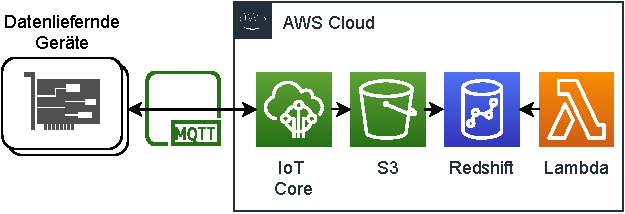
\includegraphics[width=0.8\textwidth]{graphics/Redshift-general.pdf}
\caption{Grobarchitektur des Ablaufes für Redshift}
\label{abb:GrobArchitekturRedshift}
\end{figure}
\TodoW{In Text einbauen}


\subsubsection{Features des Dienstes}
Redshift verfügt über die Funktionen \mintinline[breaklines]{sql}{APPROXIMATE PERCENTILE_DISC(percentile)} und \\ \mintinline[breaklines]{sql}{PERCENTILE_CONT(percentile)}, welche Perzentile kalkulieren können durch Annahme einer diskreten oder kontinuierlichen Datenverteilung.

Wie bereits bei Timestream und Athena gezeigt, kann \citeauthor{Salgado.2019}s Vorschlag verwendet werden, um alle Werte, ausserhalb der Spanne zwischen dem 25. und 75. Quantil liegen als Anomalie zu klassifizieren.\footcite[Vgl.][]{Salgado.2019} Obenstehende Perzentilfunktionen könnten dafür genutzt werden. Wie bereits bei Timestream und Athena vorgeschlagen, könnten auch externe Tools verwendet werden, um Anomalien mittels Machine Learning oder statistischen Methoden zu entdecken. Eine weitere Möglichkeit wäre die mittlere absolute Abweichung vom Median in einem Verarbeitungsfenster zu analysieren und größere Abweichungen als Anomalie anzuerkennen.\footcite[Vgl.][]{Peak.2017}
Schwellwertüberschreitungen können via einer \mintinline{sql}{WHERE} Bedingung, wie bei Timestream und Athena auch, erkannt werden.
Wie bei Timestream und Athena kann nach der Methode von \citeauthor{Ross.2020} ein gleitender Durchschnitt mittels der Verarbeitungsfenster kalkuliert werden.\footcite[Vgl.][]{Ross.2020}\nzitat\footcite[Vgl.][]{Ubiq.o.J.} Diese Methode wird auch von \citeauthor{Ubiq.o.J.} für Redshift vorgeschlagen.\footcite[Vgl.][]{Ubiq.o.J.}

\subsubsection{Performancegarantien}
\ac{AWS} sichert vertraglich für Redshift ebenfalls keine feste Performance im Rahmen des \acp{SLA} zu. Es werden allein Abschläge auf den zu zahlenden Preis angeboten, wenn die Verfügbarkeit des Dienstes unter 99,99\% des Monats lag.\footcite[Vgl.][]{AmazonWebServicesInc..2019b} Basierend auf den Leistungsdaten der Instanz, welche ausgewählt wurde, um Redshift zu betreiben und weiterer Faktoren, wie z.B. ob durch horizontale Skalierung mehrere Instanzen in einem Cluster zusammengefasst wurden, kann sich die Performance verändern. Zusätzlich sind wie bei vielen \ac{SQL}-basierten Datenbanken Optimierungen der Leistung durch Optimierung der gestellten Abfragen möglich.\footcite[Vgl.][]{AmazonWebServicesInc..o.J.ab} In der Erhebung von \citeauthor{Tan.2019} wurde Redshift (ohne Spectrum) ein Performancevorteil gegenüber Athena bescheinigt, während Spectrum schlechter abschnitt, als Redshift.\footcite[Vgl.][2176]{Tan.2019}


\subsubsection{Gesamtkosten}
Im Vergleich von \citeauthor{Gupta.2015}, bei dem alle Autoren \ac{AWS} angehören, bescheinigen sie Redshift ein \enquote{disruptives} Preismodell gegenüber anderer DataWarehouse Lösungen.\footcite[Vgl.][]{Gupta.2015} Ob für den Usecase dieser Arbeit Redshift ebenfalls ein \enquote{disruptives} und ansprechendes Preismodell hat, soll im Folgenden erläutert werden.

Da Redshift Spectrum durch die zusätzlich zu provisionierenden Clusterresourcen einen Kostennachteil hat, wie auch von \citeauthor{Tan.2019} festgestellt, wird von einem Kostenvergleich für Spectrum abgesehen.\footcite[Vgl.][2178]{Tan.2019}

Stattdessen werden die Kosten für ein \enquote{shared-nothing}\footcite[Vgl.][2172]{Tan.2019} Redshift \ac{OLAP} Cluster berrechnet. Dabei ist zu beachten, dass \AWSIOT{} keine direkte Regel bietet, um Daten in Redshift abzulegen. Stattdessen müssen die Daten via Kinesis Data Firehose oder \ac{AWS} Lambda eingefügt werden. Zum Zwecke der Datenübertragung wird in diesem Fall Kinesis Data Firehose kalkuliert. Wie bei Elasticsearch Service gibt es auch bei Redshift verschiedene unterliegende Instanzen zur Auswahl.\footcite[Vgl. auch im Folgenden][]{AmazonWebServicesInc..o.J.z} Im Vergleich werden, den Empfehlungen von \ac{AWS} folgend, eine Instanz der \ac{DC2} Klasse verwendet, welche sich für unkomprimierte Datenmengen kleiner ein TB eignen. Die kleinste verfügbare \ac{DC2} Instanz ist \enquote{dc2.large} mit 2 vCPUs, 15GiB Hauptspeicher und ~160 GB Festplattenspeicher. Redshift muss innerhalb eines \acp{VPC} gestartet werden, um Netzwerkisolation sicherzustellen. Aus diesem Grund ist ein Aufpreis auf Kinesis Data Firehose zu zahlen, welches Datenübertragung in ein \ac{VPC} mit einem Aufschlag berechnet.\footcite[Vgl. auch im Folgenden][]{AmazonWebServicesInc..o.J.y} Kinesis Data Firehose rundet dazu noch Daten zu den nächsten 5 KB auf, was eine effektive Datenmenge von 41,77GB ergibt.

Zusätzlich müssen Lambda Ausführung dazu gerechnet werden, die die Ausführungen der hinterlegten \ac{SQL} Abfragen zur Auswertung ausführen und danach \ac{SNS} benachrichtigen.

\begin{table}[H]
\centering
\begin{tabular}{|l|l|l|}
\hline
Dimension & Preis(\$)/Einheit & Summe (\$) \\ \hline
\begin{tabular}[c]{@{}l@{}}dc2.large Instanz\\ (OnDemand)\end{tabular} & 0,324/h & 233,60 \\ \hline
\begin{tabular}[c]{@{}l@{}}Firehose \\ Dateneingang\end{tabular} & 0,033/GB & 1,38 \\ \hline
\begin{tabular}[c]{@{}l@{}}Firehose\\ \ac{VPC}\end{tabular} & \begin{tabular}[c]{@{}l@{}}0,01/GB\\ 0,012/h\end{tabular} & 8,84 \\ \hline
Lambda Ausführungen & 0,0000002/Ausführung & 0,000192 \\ \hline
Lambda \ac{RAM} & 0,0000000167/GB-Sekunde & 0,08 \\ \hline
\ac{SNS} (Push) & \begin{tabular}[c]{@{}l@{}}0,00002/Nachricht\\ (angenommen 5 Alarme/Gerät/Monat)\end{tabular} & 0,02 \\ \hline
Summe & \cellcolor[HTML]{EFEFEF} & 243,920192 \\ \hline
\end{tabular}
\caption{Kostenvergleich Amazon~Redshift}
\label{tab:kostenvergleich-Amazon~Redshift}
\end{table}

\subsection{Amazon OpenSearch Service}

Amazon OpenSearch Service ist die verwaltetete Variante des Elasticsearch Forks von Amazon, OpenSearch.\footcite[Vgl. auch im Folgenden][]{Meadows.2021} OpenSearch Service, dessen Namensänderung weg von Elasticsearch Service im April 2021 angekündigt wurde, bietet die Datenbank Elasticsearch als Service an, welche ursprünglich von Elastic entwickelt wurde. Elasticsearch ist dabei nach Aussage des Herstellers eine verteilte, freie und offene Analytics- und Suchplattform für viele verschiedenen Datenformen.\footcite[Vgl.][]{ElasticsearchInc..o.J.} Elasticsearch basiert auf der Open Source Bibliothek Apache Lucene, welche besonders für Suchabfragen in großen Datenmengen optimiert ist. Elasticsearch ist neben Anwendungsfällen im Bereich Logverarbeitung und Monitoring auch für \ac{IIoT} Anwendungsfälle bekannt.\footcite[Vgl.][]{Mantfeld.2019}\nzitat\footcite[Vgl.][]{Bajer.2017}

\begin{figure}[H]
\centering
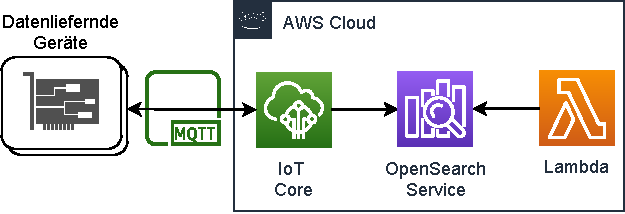
\includegraphics[width=0.8\textwidth]{graphics/OpenSearch-general.pdf}
\caption{Grobarchitektur des Ablaufes für OpenSearch Service}
\label{abb:GrobArchitekturOpenSearch}
\end{figure}
\TodoW{In Text einbauen}

\subsubsection{Features des Dienstes}
Da der OpenSearch Fork von Amazon auf der Elasticsearch Basis basiert, und \ac{AWS} explizit plant, vorest keine \ac{API} Abweichungen zur bereits bekannten \ac{API} einzubauen, werden im Folgenden die Elasticsearch Fähigkeiten dargestellt.\footcite[Vgl.][]{Meadows.2021}

Mithilfe der \enquote{Percentiles aggregation} können beliebige Perzentile eines Datensatzes berechnet werden. Dies wird in \autoref{listing:percentiles-elasticsearch} im Anhang~\ref{anhang:elastic-code} mit der Elasticsearch eigenen Abfragesprache gezeigt. 
In Elasticsearch/OpenSearch Service ist aufgrund von Amazon eigenen Anpassungen eine Anomalieerkennung basierend auf Random Cut Forest verfügbar.\footcite[Vgl.][]{AmazonWebServicesInc..o.J.al}
Alternativ lassen sich basierend auf der mittleren absolute Abweichung vom Median mit Elasticsearch eigenen Mitteln ebenfalls Aussreisser/Anomalien erkennen.\footcite[Vgl.][]{ElasticsearchInc..o.J.c} 
In der Elasticsearch eigenen Abfrage gibt es mit dem \mintinline{sql}{minimum_should_match} Parameter, eine Möglichlkeit Abfragen auf Schwellwertüberschreitungen zu stellen.\footcite[Vgl.][]{ElasticsearchInc..o.J.e}
Gleichzeitig können in Kibana/Open Search Dashboards Schwellwerte mit Alarmen konfiguriert werden.\footcite[Vgl.][]{Handler.2019}
In Elasticsearch kann ein gleitender Durchschnitt mittels der eigenen Abfragesprache kalkuliert werden. Die Berechnung kann gewichtet oder ungewichtet erfolgen.

% \begin{listing}[H]
% \inputminted[frame=lines,breaklines=true]{json}{code/elasticsearch/mavg.json}
% \caption[gleitender Durchschnitt Elasticsearch]{gleitender Durchschnitt Elasticsearch.\footnotemark}
% \label{listing:mavg-elasticsearch}
% \end{listing}
% \footnotetext{Entnommen aus: \cite{ElasticsearchInc..o.J.d}}



\subsubsection{Performancegarantien}
\ac{AWS} sichert vertraglich für OpenSearch Service ebenfalls keine feste Performance im Rahmen des \acp{SLA} zu. Auch hier werden nur Abschläge auf den zu zahlenden Preis angeboten, wenn die Verfügbarkeit des Dienstes unter 99,99\% des Monats lag.\footcite[Vgl.][]{AmazonWebServicesInc..2019} Da OpenSearch Service ein Instanzbasiertes Modell verfolgt, sind eventuelle Performanceprobleme jedoch durch einen Wechsel auf eine Instanzklasse mit stärkerer Rechenleistung (vCPUs) oder Hauptspeicher (\ac{RAM}) lösbar. Dabei zeigt der Anwendungsfall der Mayo Klinik, den \citeauthor{Chen.2017} vorstellen, dass die unterliegende Software, Elasticsearch, auch mit Datensätzen von mehr als 25 Millionen \ac{JSON}-Einträgen Anfragen mit einer Latenz von weniger als 0,2 Sekunden beantworten kann.\footcite[Vgl.][]{Chen.2017}

\subsubsection{Gesamtkosten}
Der \ac{AWS} OpenSearch Service wird auf unterliegenden \ac{EC2} Instanzen betrieben und wie diese in gewissen Klassen abgerechnet. Dabei stehen sowohl OnDemand Abrechnugsmodelle wie auch reservierte Kapazität zur Verfügung.\footcite[Vgl. auch im Folgenden][]{AmazonWebServicesInc..o.J.w} Zusätzlich steht mit \enquote{UltraWarm} eine besondere Instanzklasse zur Verfügung, welche für das Vorhalten großer Datenmengen konzipiert ist. Zusätzlich zu den Instanzen wird noch der verbrauchte \ac{EBS}-Speicherplatz abgerechnet. Dieser Speicherplatz kann in der Standard Klasse oder speziell für hohen Datendurchsatz (provisionierte \ac{IOPS}) gebucht werden. Der Speicherplatz für UltraWarm wird aber nicht via \ac{EBS} abgerechnet, sondern separat. Ebenfalls steht wieder ein \enquote{Free Tier} zur Verfügung, welches aus Vergleichsgründen nicht in die Berechnung einfliessen soll. Aus Vergleichsgründen kommen nur OnDemand abgerechnete Instanzen für den Vergleich in Frage. Für Vergleichszwecke soll eine t3.medium.elasticsearch Instanz geschätzt werden, welche mit 2 vCPUs und 4 GiB \ac{RAM} ausgestattet ist. Der provisionierte \ac{EBS}-Speicherplatz soll bei 10GB liegen.
Benachrichtigungen werden über die native Integration von Kibana (Name nach Umbenennung: OpenSearch Dashboards) und \ac{SNS} abgewickelt, wobei Kibana die Wertüberwachung übernimmt.\footcite[Vgl.][]{AmazonWebServicesInc..o.J.x}

\begin{table}[H]
\centering
\begin{tabular}{|l|l|l|}
\hline
Dimension & Preis(\$)/Einheit & Summe (\$) \\ \hline
\begin{tabular}[c]{@{}l@{}}t3.medium Instanz\\ (OnDemand)\end{tabular} & 0,084/h & 61,32 \\ \hline
\ac{EBS} Speicher & 0,161/GB & 1,61 \\ \hline
\ac{SNS} (Push) & \begin{tabular}[c]{@{}l@{}}0,00002/Nachricht\\ (angenommen 5 Alarme/Gerät/Monat)\end{tabular} & 0,02 \\ \hline
Summe & \cellcolor[HTML]{EFEFEF} & 62,95\\ \hline
\end{tabular}
\caption{Kostenvergleich Amazon~OpenSearch~Service}
\label{tab:kostenvergleich-Amazon~Elasticsearch~Service}
\end{table}



\subsection{Auswahl}
Der von \citeauthor{Tan.2019} konstatierte Preisvorteil von Redshift gegenüber Athena hat sich in dem durchgeführten Vergleich nicht gezeigt.\footcite[Vgl.][2178\psq]{Tan.2019} Dies könnte womöglich dem Fakt geschuldet sein, dass die Datenmengen der Studie einen \enquote{Break-even} Punkt überschritten haben, an dem das Athena Abrechnungsmodell im Vorteil gegenüber Redshift war.
Die Performance der verglichenen Dienste variierte aufgrund verschiedener unterliegender Faktoren, wie beispielsweise provisionierter Leistung oder der Optimierung für spezifische Anfragen, was andere Anfragen verlangsamte. Letzten Endes ist es fraglich, ob \ac{OLAP} Analysen, die zeitgesteuert erstellt werden eine garantierte Performance im Sub-Sekunden Bereich brauchen, oder ob es reicht, die Analyse in längerer Zeit zu erledigen, da die Daten sowieso zeitversetzt sind.
Übertragbare Dienste/Produkte sind Amazon OpenSearch und Amazon Athena. OpenSearch, welches größtenteil Kompatibilität zu ElasticSearch hat (mit Ausnahme des Amazon eigenen Anomalieeerkennungsplugins) kann mit Anpassungen mit dem ElasticSearch Code in anderen Public Clouds verwendet werden. Da Athena auf Presto basiert, sind Abfragen kompatibel und portabel. Dies erfordert entsprechende Unterstützung für Presto in der Zielcloud oder eine eigene Installation.
Bei den verglichenen Diensten handelt es sich mit Ausnahme von OpenSearch um von Amazon teilweise oder komplett entwickelte properitäre Dienste, weshalb die Integration mit anderen \ac{AWS} Dienstleistungen gegeben ist. Auch OpenSearch wird mittlerweile, als Fork von Elasticsearch, hauptsächlich von \ac{AWS} betreut und ist bereits gut mit anderen Dienstleistungen integriert.
Auch wenn die verglichenen Datenbankdienste für jeweils individuelle Zwecke entwickelt wurden, sind sie doch generalisiert für mehrere Usecases verwendbar und erweiterbar.
Im Bereich Fehlertransparenz gab es Abzug für Athena, da fehlschlagende Abfragen nur mit generischen Fehlermeldungen beantwortet werden, was die Fehlersuche erschwert.
Punktabzüge im Wartungsaufwand und der Skalierbarkeit gab es für die auf Instanzen basierenden Dienste OpenSearch und Redshift, welche durch die von Nutzenden vorzunehmende vertikale Skalierung einen höheren Wartungs- und Überprüfungsaufwand fordern, als Timestream und Athena, die verwaltet sind.
Die Gesamtkosten scheinen bei Redshift zumindest im vorliegenden Fall, ohne konkrete Optimierungen besonders hoch zu sein, genauso wie bei Athena. Kostenführer ist Timestream, gefolgt von OpenSearch Service.
Alle verglichenen Dienste können die Auswertungen in angemessener Zeit anfertigen. 
Athena hat Punktabzüge im Bereich Robustheit \& Fehlertoleranz, da ein sich veränderndes Datenschema zu schwerwiegenderen Problemen führen kann.
Alle Dienste bieten die gewünschten Auswertungen an. Technisch sind aufgrund der unterschiedliche Implementierungen trotzdem Unterschiede vorhanden.


\begin{table}[H]
    \centering
    \begin{tabular}{|l|l!{\vrule width 2pt}l|l|l|l|}
    \hline
\multicolumn{1}{|c|}{Kriterium} & \multicolumn{1}{c!{\vrule width 2pt}}{\begin{tabular}[c]{@{}c@{}}max.\\Punkte\end{tabular}} & \multicolumn{1}{c|}{\begin{tabular}[c]{@{}c@{}}Amazon\\Timestream\end{tabular}} & \multicolumn{1}{c|}{\begin{tabular}[c]{@{}c@{}}Amazon\\OpenSearch\end{tabular}} & \multicolumn{1}{c|}{\begin{tabular}[c]{@{}c@{}}Amazon\\Athena\end{tabular}} & \multicolumn{1}{c|}{\begin{tabular}[c]{@{}c@{}}Amazon\\Redshift\end{tabular}} \\ \hline
     \begin{tabular}[c]{@{}l@{}}Übertragbarkeit zwischen \\ Clouds (ISO 9126)\end{tabular} & 1 & 0 & 1 & 1 & 0 \\ \hline
     \begin{tabular}[c]{@{}l@{}}Integration mit anderen \\ \ac{AWS} Diensleistungen\end{tabular} & 3 & 3 & 3 & 3 & 3 \\ \hline
     Generalisierung & 4 & 4 & 4 & 4 & 4 \\ \hline
     Erweiterbarkeit & 4 & 4 & 4 & 4 & 4 \\ \hline
     \begin{tabular}[c]{@{}l@{}}Fehlertransparenz/ \\ Debugability\end{tabular} & 5 & 5 & 5 & 4 & 5 \\ \hline
     \begin{tabular}[c]{@{}l@{}}geringer \\ Wartungsaufwand\end{tabular} & 7 & 7 & 5 & 7 & 5 \\ \hline
     \begin{tabular}[c]{@{}l@{}}Skalierbarkeit \& \\ \enquote{serverlessness}\end{tabular} & 7 & 7 & 5 & 7 & 5 \\ \hline
     Kosten & 7 & 7 & 6 & 5 & 4 \\ \hline
     Performancegarantien & 8 & 8 & 8 & 8 & 8 \\ \hline
     \begin{tabular}[c]{@{}l@{}}Robustheit \& \\ Fehlertoleranz\end{tabular} & 9 & 9 & 9 & 6 & 9 \\ \hline
     \begin{tabular}[c]{@{}l@{}}Auswertungen \\ (\autoref{chap:auswertungsarten}) \end{tabular} & 11 & 11 & 11 & 11 & 11 \\ \hlinewd{2pt}
     \rowcolor[HTML]{ECF4FF}
     Summe & 66 & \textbf{\cellcolor[HTML]{ECF4FF}65} & \textbf{\cellcolor[HTML]{ECF4FF}61} & \textbf{\cellcolor[HTML]{ECF4FF}60} & \textbf{\cellcolor[HTML]{ECF4FF}58} \\ \hline
\end{tabular}
\caption{Bewertungsmatrix~Batch}
\label{tab:bewertungsmatrix-batch}
\end{table}



\section{Dienste, die mehrere Modi unterstützen}
Aufgrund der hohen Popularität der $\lambda$-Architektur, gibt es Dienste, die sowohl Echtzeitverarbeitung, als auch Batch/\ac{OLAP}-Verarbeitung unterstützen.

\subsection{AWS IoT Analytics} \label{productselection:iotanalytics}



\AWSIOT{} Analytics ist ein Dienst der \AWSIOT{} Familie, der nach Aussage des Herstellers weitreichende Analysen von \ac{IoT} Daten, die beispielsweise via \AWSIOT{} Core geladen werden können, zulässt.\footcite[Vgl. auch im Folgenden][]{AmazonWebServicesInc..o.J.c} Dabei bietet der Dienst Lösungen für Sammlung, Verarbeitung, Speicherung, Analyse und Benachrichtigung/Visualisierung von Daten an, bzw. bietet Schnittstellen, um diese Aufgaben zu erledigen. Im speziellen deckt \AWSIOT{} Analytics die Aufgaben einer $\lambda$-Architektur ab. So besitzt \AWSIOT{} Analytics beispielsweise eine integrierte Zeitreihendatenbank, welche ergänzend zu den Echtzeitdaten von \AWSIOT{} Core für Analysen genutzt werden kann.
\begin{figure}[H]
\centering
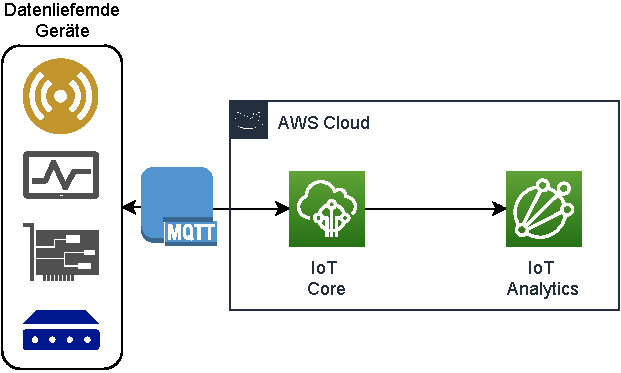
\includegraphics[width=0.8\textwidth]{graphics/IoT-Analytics-general.pdf}
\caption{Grobarchitektur des Ablaufes für IoT Analytics}
\label{abb:GrobArchitekturIoTAnalytics}
\end{figure}
In \autoref{abb:GrobArchitekturIoTAnalytics} ist die Grobarchitektur und Verknüpfung mit anderen Diensten unter Annahme der Vorraussetzungen aus \autoref{chap:rahmendatenverarbeitung} gezeigt. Datenliefernde Geräte, wie beispielsweise Sensoren, liefern Zeitreihen-Messwerte via dem \ac{MQTT} Protokoll an. Die Weiterleitung zu IoT Analytics erfolgt mittels einer eingerichteten Regel im \ac{IoT} Core Messagebroker, welche mittels eines Dialekts der \ac{SQL} Sprache gewisse Topics vorselektiert oder alle Topics zulässt.


Für erweiterte Analysen stellt \AWSIOT{} Analytics sogenannte Notebooks zur Verfügung, die auf den \enquote{Jupyter Notebooks} basieren. Diese Notebooks werden verwendet, um Python Programmabläufe zu visualieieren und zu modularisieren. Da in den Jupyter Notebooks der volle Paketumfang von Python verfügbar ist, inklusive z.B. Machine Learning Bibliotheken wie Tensorflow, sind wesentlich erweiterte Analysen möglich. Die Ressourcen für Notebooks sind seperat zu provisionieren und werden in Analytics Compute Units abgerechnet, wobei eine Compute Unit 4vCPU-Kerne und 16 GB \ac{RAM} hat.\footcite[Vgl.][]{AmazonWebServicesInc..o.J.i} Diese Compute Units werden sekundengenau abgerechnet und kosten nur für die Laufzeit Geld.

\subsubsection{Gesamtkosten}
In \autoref{tab:kostenvergleich-AWS~IoT~Analytics} sind die kalkulierten Preise nach gängiger Preismatrix dargestellt.\footcite[Vgl. auch im Folgenden][]{AmazonWebServicesInc..o.J.i} Die Nutzung von externen Ausführungsdiensten (z.B. StepFunctions/Lambda) für \ac{SQL}-Abfragen ist nicht notwendig, da die Abfragen im Dienst selbst terminiert werden können.
\begin{table}[H]
\centering
\begin{tabular}{|l|l|l|}
\hline
Dimension & Preis(\$)/Einheit & Summe (\$) \\ \hline
Datenspeicherung (roh+verarbeitet)  & \begin{tabular}[c]{@{}l@{}}0,03/GB (verarbeitet) \\ 0,023 (roh)\end{tabular} & 7,77  \\\hline
Anfragenbearbeitung & \begin{tabular}[c]{@{}l@{}}0,00634/GB\end{tabular} & 121,50 \\ \hline
\begin{tabular}[c]{@{}l@{}}Eigene Analyselogik \\ 960 Abfragen * 5 Sekunden\end{tabular}  & 0,36/h & 0,48  \\\hline
Summe & \cellcolor[HTML]{EFEFEF} & \underline{129,75}  \\\hline

\end{tabular}
\caption{Kostenvergleich AWS~IoT~Analytics}
\label{tab:kostenvergleich-AWS~IoT~Analytics}
\end{table}
 Das bestehende \enquote{Free Tier}, welches \ac{AWS} für den Dienst anbietet, wird ignoriert, da es nur in den ersten zwölf Monaten der Nutzung des Dienstes verrechnet wird. Bei \ac{S3} wird angenommen, dass die Standard Speicherklasse verwendet wird und Volumenrabattierungen bei Datenvolumina >50TB im Monat nicht relevant sind.\footcite[Vgl. auch im Folgenden][]{AmazonWebServicesInc..o.J.j} Andere Speicherklassen sind günstiger, somit gibt die Schätzung eine Obergrenze für die \ac{S3} Preise. Es wurde ebenfalls keine eigene Logik in Notebooks kalkuliert, welche 0,36\$ pro Stunde und Compute Unit im Betrieb kosten würden. Dies ist dem Fakt geschuldet, dass für dieses Beispiel die Analysen mit \ac{SQL} bewältigbar sind.
 
\subsubsection{Weitere Evaluationen}
Die Performance und Verfügbarkeit sowie die Features werden in \anhangref{anhang:vergleich-iot-analytics} diskutiert.

\subsection{Auswahl}
Im Bereich Multimode gibt es nur einen zu vergleichenden Dienst, weshalb Abzüge nicht auf relativen Kriterien zu den anderen Diensten basieren, sondern auf absoluten Abzügen.
\begin{table}[H]
    \centering
    \begin{tabular}{|l|l!{\vrule width 2pt}l|}
    \hline
\multicolumn{1}{|c|}{Kriterium} & \multicolumn{1}{c!{\vrule width 2pt}}{\begin{tabular}[c]{@{}c@{}}max.\\Punkte\end{tabular}} & \multicolumn{1}{c|}{\begin{tabular}[c]{@{}c@{}}AWS\\IoT\\Analytics\end{tabular}} \\ \hline
     \begin{tabular}[c]{@{}l@{}}Übertragbarkeit zwischen \\ Clouds (ISO 9126)\end{tabular} & 1 & 0 \\ \hline
     \begin{tabular}[c]{@{}l@{}}Integration mit anderen \\ \ac{AWS} Diensleistungen\end{tabular} & 3 & 3 \\ \hline
     Generalisierung & 4 & 3 \\ \hline
     Erweiterbarkeit & 4 & 4 \\ \hline
     \begin{tabular}[c]{@{}l@{}}Fehlertransparenz/ \\ \textit{Debugability}\end{tabular} & 5 & 4 \\ \hline
     \begin{tabular}[c]{@{}l@{}}geringer \\ Wartungsaufwand\end{tabular} & 7 & 4 \\ \hline
     \begin{tabular}[c]{@{}l@{}}Skalierbarkeit \& \\ \textit{serverlessness}\end{tabular} & 7 & 6 \\ \hline
     Kosten & 7 & 5 \\ \hline
     Performancegarantien & 8 & 7 \\ \hline
     \begin{tabular}[c]{@{}l@{}}Robustheit \& \\ Fehlertoleranz\end{tabular} & 9 & 7 \\ \hline
     \begin{tabular}[c]{@{}l@{}}Auswertungen \\ (\autoref{chap:auswertungsarten}) \end{tabular} & 11 & 11 \\ \hlinewd{2pt}
     \rowcolor[HTML]{ECF4FF}
     Summe & 66 & \textbf{\cellcolor[HTML]{ECF4FF}54} \\ \hline
\end{tabular}
\caption{Bewertungsmatrix~Multimode}
\label{tab:bewertungsmatrix-multimode}
\end{table}
Klar ist, dass zwar bei \AWSIOT{} Analytics die Jupyter Notebooks plattformunabhängig sind, aber die \ac{SQL}-Statements nicht übertragbar sind und zwingend ein \AWSIOT{} Core Broker benötigt wird. Aufgrund dieses \textit{vendor-lockins} kann ein großer Teil des Setups nicht übertragen werden.
\AWSIOT{} Analytics integriert sich gut mit anderen Dienstleistungen von AWS, z.B. mit \AWSIOT{} Core und den anderen \AWSIOT{} Diensten, SageMaker, QuickSight , Lambda, \ac{SNS} und weiteren.
\AWSIOT{} Analytics ist speziell für \ac{IoT} Daten gebaut, weshalb Funktionalitäten eingebaut sind, die speziell in Kombination mit den anderen \AWSIOT{} Diensten Sinn machen. Die Verwendung dieser Funktionalitäten ist aber nicht zwingend notwendig. Es können auch andere Daten, z.B. IT-Monitoring eingespeist werden, wenn sie über \ac{MQTT} und den \AWSIOT{} Core Broker geladen werden.
Die Erweiterbarkeit ist gegeben durch die Möglichkeiten, die \ac{SQL} in Verbindung mit der generischen Programmierbarkeit der Notebooks bietet und zusätzlich dadurch, dass durch die integrierte Datenbank Daten erneut mit anderer Logik verarbeitet werden können.
Durch Integration mit Cloudwatch, der Monitoring Lösung von \ac{AWS} sind ansteigende Fehlerraten leicht zu entdecken. Einzig, dass eingehende Daten einige Zeit benötigen, bis sie von der \AWSIOT{} Analytics Konsole angezeigt werden, kann die Fehlersuche erschweren.\footcite[Vgl.][]{AmazonWebServicesInc..o.J.aw}
Im Bereich \enquote{serverlessness} wurden Abzüge getätigt, da Analyitcs Compute Units nicht selbstständig skalieren.
Da die Abfragekosten mittels \ac{SQL} proportional zu den anderen Kosten hoch erscheinen, wurden Abzüge gemacht.
Die gesetzten Performancelimits des Dienstes erscheinen sinnvoll. Eine Fehlertoleranz ist gegeben, wenn der Anwender keine Fehler selbst einführt, oder \AWSIOT{} Analytics interne Fehler aufweist. Da alle Auswertungen sogar in multiplen Wegen machbar sind, wurde die volle Punktzahl für diese Kategorie vergeben. Im Vergleich zu den spezialisierteren Diensten, die dem $kappa$ oder \ac{OLAP} Muster folgen, schneidet \AWSIOT{} Analytics schlechter ab. Dies ist bedingt durch die wesentlich höheren monatlichen Kosten, genauso wie durch eine fehlende Garantie der schnellen Datenverarbeitung, zu welcher Kinesis fähig ist. Das $lambda$ Pattern scheint in dieser Implementierung ein nachteiliger Kompromiss aus der Kombination von $kappa$ und \ac{OLAP} zu sein.

\subsubsection{Übertragbarkeit zwischen Clouds}
\subsubsection{Integration mit AWS}
\subsubsection{Generalisierung}
\subsubsection{Erweiterbarkeit}
\subsubsection{Fehlertransparenz}
\subsubsection{geringer Wartungsaufwand}
\subsubsection{Skalierbarkeit \& serverlessness}
\subsubsection{Kosten}
\subsubsection{Performancegarantien}
\subsubsection{Robustheit \& Fehlertoleranz}
\subsubsection{Auswertungen}
\subsubsection{Summe}





\chapter{Modellierung}
In diesem Kapitel sollen die Anforderungen aus den Interviews praktisch erhoben, die Referenzarchitekturen erstellt und die konstruierten Referenzarchitekturen folgend auch verglichen werden.
\section{Anforderungserhebung}
Wie in \autoref{theorie:referenzmodellierung} beschrieben, müssen Referenzmodelle einen subjektiven Empfehlungscharakter besitzen, damit sie akzeptiert und wiederverwendet werden. Dafür muss ein Abgleich mit den Anforderungen der Nutzenden geschehen. Um dies zu erreichen, wurden im Anhang transkribierte Interviews (vgl. \anhangref{anhang:interview-philipp-22.03.2021}, \anhangref{anhang:interview-peter-24.03.2021}, \anhangref{anhang:interview-ralph-24.03.2021}) durchgeführt. Daraus ergibt sich das in \autoref{abb:TopLevelEchtzeitRA} gezeigte Diagramm, welches die Anforderungen der individuellen Stakeholder an Dekompositionstiefe, Anwendbarkeit und Allgemeingültigkeit darstellt.

\begin{figure}[H]
\centering
\spideroverview
%{P. Arnold}
{5}{3}{3}
%{R. Briegel}
{3}{3}{1}
%{P. Erbacher}
{2}{4}{5}
\caption{Ergebnisse der Interviews}
\label{abb:DimensionenUebersicht}
\end{figure}
Durch die Interviews liessen sich folgende Durchschnitte errechnen: Dekompositionstiefe wurde im Schnitt mit $3,\overline{3}$ bewertet. Die Anwendbarkeit wurde ebenfalls mit $3,\overline{3}$ bewertet. Die Allgemeingültigkeit hingegen hat nur einen Schnitt von $3$. Entsprechend sollten Dekompositionstiefe und Anwendbarkeit priorisiert werden, während die Referenzarchitektur organisationsspezifischer sein darf. 
In den folgenden Referenzarchitekturen wird in mehrere Dekompositionen unterteilt. In der Datenverarbeitungssequenz werden mit Hilfe eines Sequenzdiagramms die Abläufe zur Datenverarbeitung mit dem zu betrachtenden Dienst, ausgehend von \AWSIOT{} Core als Messagebroker gezeigt.
Die Verteilungssicht soll sowohl die Interaktion der Dienste untereinander, als auch grob das durchzuführende Deployment zeigen. Die Bausteinsicht zeigt wichtige Elemente der einzelnen Dienste auf, die konkret untereinander interagieren. So ist die konkrete Untereinheit, die Daten von \AWSIOT{} Core an andere Dienste versendet eine \AWSIOT{} Core Rule, welche aufzuzeigen wäre. \TodoW{Genauere Auswirkungen}

Für die Operations wird vorausgesetzt, dass der \ac{AWS}-native Dienst CloudWatch zur Überwachung eingesetzt wird. 
\begin{figure}[H]
\centering
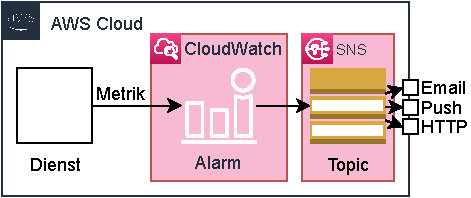
\includegraphics[width=0.66\textwidth]{graphics/CloudWatch-Monitoring}
\caption{CloudWatch Monitoring}
\label{abb:CloudWatchMonitoring}
\end{figure}
CloudWatch erfasst zentralisiert Metriken aller Dienste und löst bei nutzerdefinierten Überschreitungen einen Alarm aus, welcher dann via \ac{SNS} versendet werden kann (siehe \autoref{abb:CloudWatchMonitoring}). Dabei kann bei Metriken mit hoher Varianz die Cloudwatch eigene Anomalienerkennung verwendet werden oder die Schwellwerterkennung.



Zusätzlich haben sich folgende Anforderungen ergeben:
\begin{itemize}
\item Anwendbarkeit auf Monitoringdaten (IT) (\anhangref{anhang:interview-philipp-22.03.2021}, \anhangref{anhang:interview-peter-24.03.2021})
\item Anwendbarkeit auf Sensordaten (\ac{IoT}) (\anhangref{anhang:interview-philipp-22.03.2021}, \anhangref{anhang:interview-peter-24.03.2021}, \anhangref{anhang:interview-ralph-24.03.2021})
\item Wertschöpfung für das Unternehmen wichtig
\item akzeptabel und problemlösend für Domäne
\item Handling von Events, Messwerten und \enquote{Streaming} (\anhangref{anhang:interview-peter-24.03.2021})
\end{itemize}

% \begin{figure}[H]
% \centering
% 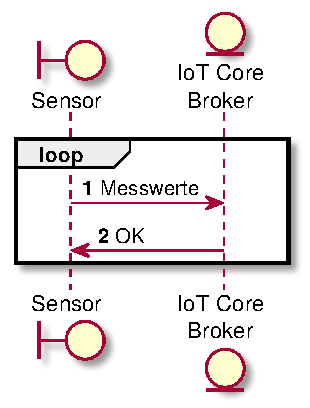
\includegraphics[height=0.3\textheight]{graphics/dateneinspeisung.pdf}
% \caption{Sequenzdiagramm Dateneinspeisung}
% \label{abb:SequenceEinspeisung}
% \end{figure}

Im Folgenden werden die Referenzarchitekturen entworfen und miteinander verglichen, um mögliche Stärken und Einsatzgebiete zu identifizieren.

\section{Echtzeitverarbeitung}\label{chap:ra-rt}
Aufgrund des in \autoref{tab:bewertungsmatrix-echtzeit} durchgeführten Vergleiches, den Kinesis (Data Streams und Analytics) anführte, wird im Folgenden die Referenzarchitektur für die Echtzeitverarbeitung mit Kinesis Data Streams und Analytics entworfen. Diese Referenzarchitektur entspricht dem in \autoref{chap:bestehende_ras} vorgestellten Konzept einer $\kappa$-Architektur.

\subsection{Datenverarbeitungssequenz}
In \autoref{abb:SequenceEchtzeitRA} wird die durchlaufene Sequenz für eingehende Daten gezeigt. Nach initialer Übertragung via \ac{MQTT} an \AWSIOT{} Core, folgt die Übertragung in Kinesis Data Streams, welche die Daten gepuffert an Kinesis Data Analytics sendet. 

\begin{figure}[H]
\centering
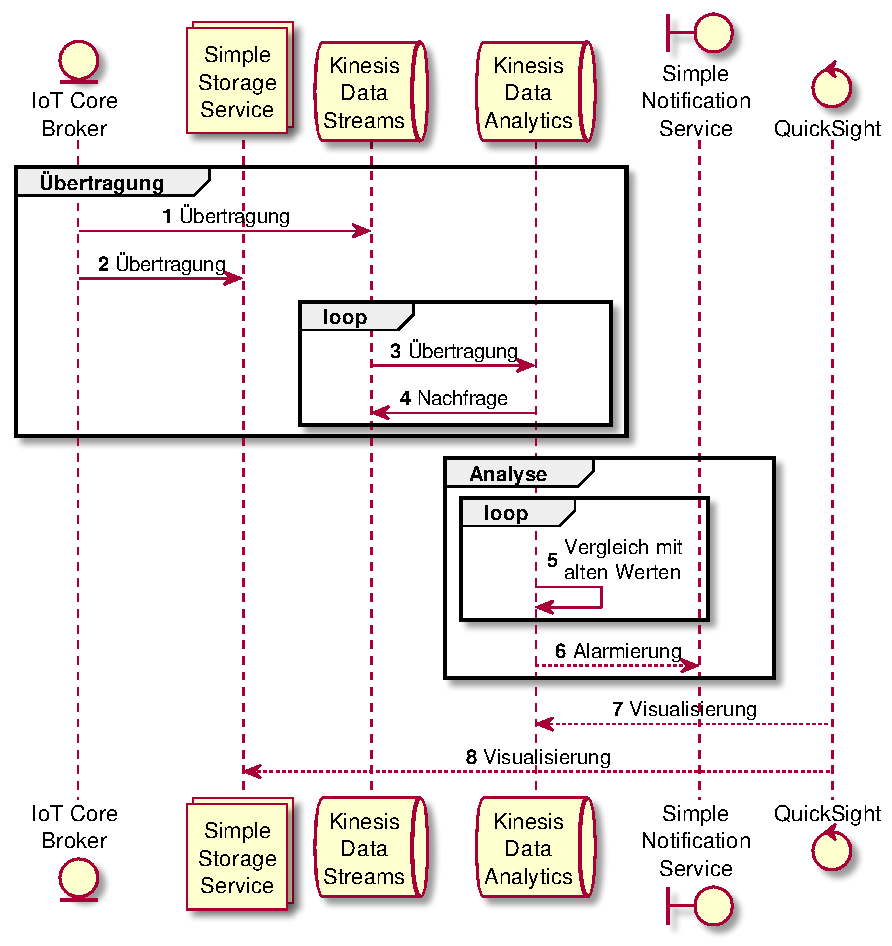
\includegraphics[height=0.6\textheight]{graphics/echtzeit-ra.pdf}
\caption{Sequenzdiagramm Echtzeitreferenzarchitektur}
\label{abb:SequenceEchtzeitRA}
\end{figure}

\subsection{Verteilungssicht}
Folgend ist die Verteilungssicht der Echtzeitreferenzarchitektur gezeigt. Gemeinsame Variationspunkte dieser und folgender Dekompositionen bekommen den Buchstaben G und eine fortlaufende Nummer und werden nur einmal erklärt.
\begin{figure}[H]
\centering
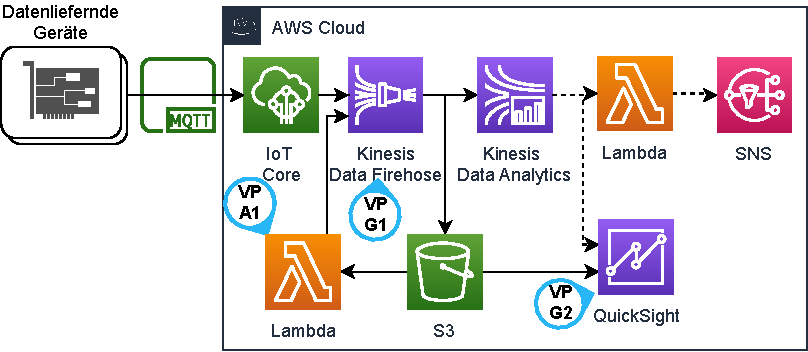
\includegraphics[width=\textwidth]{graphics/Echtzeit-RA-Overview-Firehose}
\caption{Verteilungssicht mit Data Firehose}
\label{abb:TopLevelEchtzeitRA}
\end{figure}

\vp{G1}: Je nach Anforderung kann Kinesis Data Firehose oder Kinesis Data Streams verwendet werden. Während die höhere Abstraktion und das einfachere Abrechnungsmodell von Kinesis Data Firehose einen reduzierten Wartungsaufwand hat, bietet Kinesis Data Streams mehr Kontrolle über unterliegende Faktoren wie Datenaufbewahrung und Durchsatz. Kinesis Data Firehose benötigt zwingend ein \enquote{Delivery ziel}. Dies kann beispielsweise ein \ac{S3}-Bucket, eine Redshift Datenbank oder eine Elasticsearch Datenbank sein. In diesem Fall wurde aus Kosten- und Umsetzungserwägungen ein \ac{S3}-Bucket gewählt.



\vp{G2}: QuickSight als \ac{AWS} native Dashboardlösung ist gut geeignet, um schnell Übersicht in Datenanalysen aus Kinesis Data Analytics zu bekommen. Alternativ können auch andere Visualisierungslösungen wie Tableau eingesetzt werden, welche gegebenenfalls jedoch keinen (vollen) Zugriff auf Kinesis Data Analytics haben. Ein weiterer managed Service, den \ac{AWS} für Dashboards anbietet, ist der Amazon Managed Service for Grafana, welcher das Open Source Visualisierungstool Grafana mit den \ac{AWS} eigenen Metriken integriert.\footcite[Vgl.][]{Dutt.2020} In diesem Fall kann der \ac{S3} Bucket verwendet werden, um Dashboards über die Rohdaten zu erstellen. 

\vp{A1}: Sollte es nicht gewünscht sein, Daten erneut in Kinesis Data Firehose einzuspielen, kann auf die Lambdafunktion verzichtet werden. Diese liest, wenn manuell aktiviert, den \ac{S3}-Speicher ein und spielt die erfassten Nachrichten erneut in der selben Sequenz in Kinesis Data Firehose ein. Notwendig wird diese Lambda, wenn historische Daten mit abweichender Analyselogik analysiert werden sollen.

Im Folgenden wird die Verteilungssicht im zweiten Fall von \vpref{G1}, der Verwendung von Kinesis Data Streams gezeigt. Die Auswahl von Kinesis Data Streams ist insbesondere angezeigt, wenn die Nachrichten direkt aufbewahrt werden sollen und direkter Einfluss auf die Performance erwünscht ist.

\begin{figure}[H]
\centering
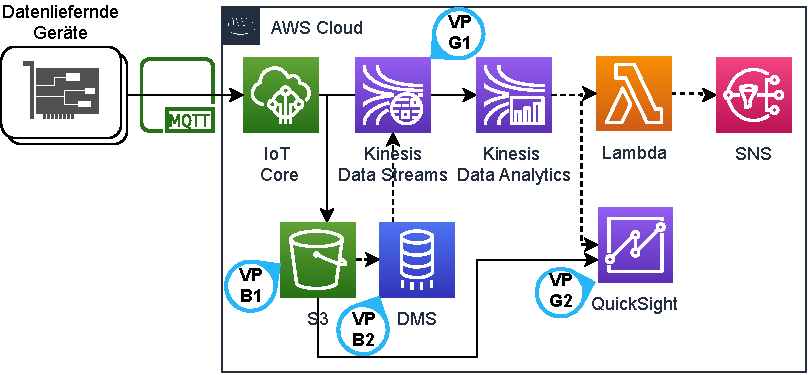
\includegraphics[width=\textwidth]{graphics/Echtzeit-RA-Overview.pdf}
\caption{Verteilungssicht mit Data Streams}
\label{abb:TopLevelEchtzeitRAStreams}
\end{figure}

\textbf{Variationspunkte G1, G2}: Siehe oben: \vpref{G1}, \vpref{G2}

\vp{B1}: Rohdaten in \ac{S3} zu speichern kann Sinn machen, um die Daten später noch einmal analysieren zu können. Nimmt man aber die Theorie der Datenhalbwertszeit zur Hilfe, macht es vielleicht Sinn die Daten statdessen maximal 48h in Kinesis Data Streams zwischenzuspeichern und auf \ac{S3} zu verzichten. Mittels der erweiterten Aufbewahrung $\lbrack$\textit{Data Retention}$\rbrack$ können Analysen mehrfach im Fehlerfall angefordert werden. Da die Preise nach sieben Tagen Aufbewahrung ansteigen und für Aufbewahrung und Abruf doppelt abgerechnet wird, ist zu empfehlen, nach sieben Tagen die Daten zu verwerfen.\footcite[Vgl.][]{AmazonWebServicesInc..o.J.l} Dieser Variationspunkt ist abhängig vom \vpref{G1}, da Kinesis Data Firehose keine erweiterte Aufbewahrung unterstützt und die Daten in \ac{S3} abgelegt werden müssen.

\vp{B2}: \ac{DMS} ist in diesem Szenario dafür gedacht, einmal abgelegte Daten in S3 wieder in Kinesis Data Streams einspielen zu können. Je nach Szenario ist dies, wie bei \vpref{B1} schon erläutert, nicht notwendig.

\subsection{Bausteinsicht}
Unter Berücksichtigung von \vpref{G1} gibt es zwei Bausteinsichten. Dies ist bedingt durch die sich ergebenden architekturellen Änderungen, beim Einsatz von Kinesis Data Streams oder Kinesis Data Firehose. 

\begin{figure}[H]
\centering
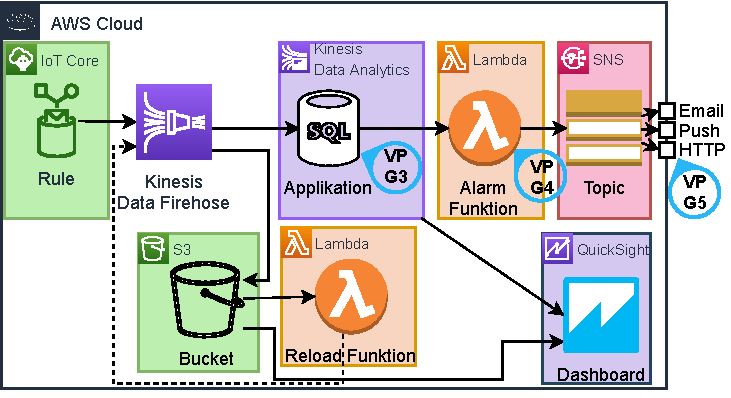
\includegraphics[width=\textwidth]{graphics/Echtzeit-RA-Elements-Firehose.pdf}
\caption{Bausteinsicht mit Data Firehose}
\label{abb:ElementeEchtzeitRA}
\end{figure}

\vp{G3}: Der \ac{SQL} Programmcode, der in Kinesis Data Analytics läuft ist anzupassen. So sind Verarbeitungsfenster, Attributsnamen und aufgerufene Funktionen nach Anforderung zu ändern. Andernfalls kann auch die Funktionalität zur Ausführung eigenen Codes via Apache Flink in Kinesis Data Analytics genutzt werden (dies erlaubt Ausführung von Java, Scala, Python). Dies ist angezeigt, wenn der \ac{SQL}-Dialekt die gewünschten Auswertungen nicht unterstützt, oder eine eigene Implementierung vorgesehen ist.

\vp{G4}: Aufgrund der Notwendigkeit einer Lambda Funktion, um Alarme zu versenden, kann der Code selbst gestaltet werden. Wichtig ist dabei, dass Kinesis Data Analytics die Zustellung von Datensätzen wiederholt, wenn die Lambdafunktion als Rückgabewert ein Array mit den Ids und dem Status wie folgt zurückgibt: \mintinline[breaklines]{json}{[{"recordId": "<ID>", "result": "DeliveryFailed"}]}.\footcite[Vgl.][]{AmazonWebServicesInc..o.J.ay} Die übermittelten Alarme lassen dabei Möglichkeit zur Anpassung. So kann neben dem Titel der Nachricht auch der eigentliche Inhalt angepasst werden. Beispielhaft ist in \anhangref{anhang:echtzeit-codesample} gezeigt, wie eine in JavaScript geschriebene Lambdafunktion aussehen könnte, die via Kinesis Data Analytics angesteuert wird. Diese Funktion gibt selbstständig fehlerhafte Nachrichten zur Wiederverarbeitung an Kinesis Data Analytics zurück, versendet \ac{SNS} Alarme und kann via \ac{MQTT} eine Shutdown Nachricht an das Gerät übermitteln.

\vp{G5}: \ac{SNS} unterstützt mehrere Protokolle für die Übermittlung von Nachrichten. Es können HTTP Webhooks genauso wie mobile Pushbenachrichtigungen oder auch Emails versendet werden. Welches Protokoll mit welchem Verteiler zu wählen ist, muss im \ac{SNS} Topic eingestellt werden. Innerhalb der Cloud Native Solution der SPIRIT/21 hat sich bewährt, den Versand via Email zu nutzen und als Ziel den Email-Verteiler eines Monitoring Teams innerhalb des Tools Microsoft Teams einzustellen. Microsoft Teams zeigt eingegangene Emails an den Emailverteiler dann als Chatnachricht innerhalb des Teams an und benachrichtigt alle Teilnehmenden.

\begin{figure}[H]
\centering
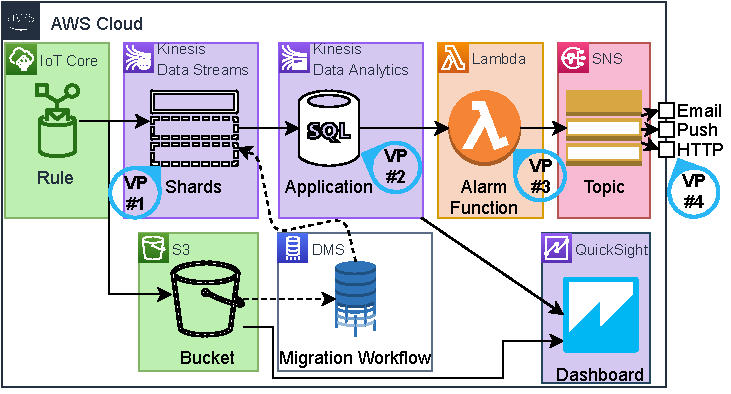
\includegraphics[width=\textwidth]{graphics/Echtzeit-RA-Elements.pdf}
\caption{Bausteinsicht mit Data Streams}
\label{abb:ElementeEchtzeitRAStreams}
\end{figure}
\textbf{Variationspunkte G3, G4, G5}: Siehe oben: \vpref{G3}, \vpref{G4}, \vpref{G5}

\vp{C1}: Die Anzahl an Shards ist essentiell für die Performance von Kinesis Data Streams. Für Workloads mit einem vorhersehbaren Workload ist Anzahl an Shards nach einem Preis/Leistungs Optimum zu ermitteln und zu konfigurieren. Wenn der Workload nicht vorhersehbar ist oder schnell skalieren können soll, sind Alarme im AWS eigenen Monitoring Tool CloudWatch zu erstellen. Im Beispielusecase für die Kostenschätzung ist ein einziger Shard (1MiB/Sekunde, 1000 Nachrichten eingehend) ausreichend. Dies ist bedingt, da Nachrichten mit einer Größe von 1KB, also ca. 1KiB geschrieben werden, bei einem Maximum von 200 pro Sekunde und einem Konsumenten. Es ist besonders auf die \enquote{WriteProvisionedThroughputExceeded} Metrik zu achten, welche bei höheren Werten anzeigt, dass das Hinzufügen von zusätzlichen Shards angebracht wäre. Ebenfalls ist die Metrik \enquote{Incoming Records} zu beachten. Verändert diese sich, deutet das auf einen Fehler im vorgelagerten \AWSIOT{} Core oder in einem Teil der Datenlieferanten hin.

\subsection{Anforderungen}
\begin{itemize}
\item Anwendbarkeit auf Monitoringdaten (IT)\\
Kinesis als System ist gut auf diverse Zeitseriendaten anwendbar. Problematisch ist das eigene Übertragungsformat, welches von Datenproduzenten verlangt, spezielle Schnittstellen zu implementieren. Der von \ac{AWS} vorgesehene Weg, die Kinesis Producer Library ist in Java geschrieben und bindet eine ausführbare C++ Datei ein.\footcite[Vgl.][]{AmazonWebServicesInc..o.J.bg} Im Einsatz mit Monitoringdaten würde dies erfordern, dass die Daten in einem Standardformat aggregiert und dann mittels eines in Java geschriebenen Programms transformiert werden müsste. 
% Alternativ können noch die \enquote{Kinesis Record Aggregation \& Deaggregation Modules for AWS Lambda} von \ac{AWS} verwendet werden, welche die Daten in das aggregierte, kinesiseigene Format umwandeln.\footnote{Siehe \url{https://github.com/awslabs/kinesis-aggregation}} Diese Module haben Sprachkompatibilität zu Java, JavaScript/Node.js und Python.
CloudWatch bietet genau diese Funktionalität mittels der CloudWatch Metric Streams und der CloudWatch Log Subscriptions an.\footcite[Vgl. auch im Folgenden][]{Barr.2021} Bei Metric Streams werden Metriken auf Wunsch in das OpenTelemetry oder das \ac{JSON} Format konvertiert und dann an Kinesis Data Firehose zur Weiterverarbeitung übermittelt. Dabei werden aber nur Metriken erfasst, die einen Zeitstempel jünger als zwei Stunden haben, was manche Metriken, die einmal am Tag versendet werden ausschließt. Zusätzlich muss ein Metric Stream in jeder Region angelegt werden, wo CloudWatch Logs anfallen, was eine Herausforderung in stark verteilten \ac{AWS}-Accounts darstellen kann. Metric Streams kosten 0,003\$ pro 1000 verarbeitete Metriken und zusätzlich die entsprechend anfallenden Data Firehose Gebühren. CloudWatch Log Subscriptions bietet sowohl das Streamen an Kinesis Data Streams, als auch an Kinesis Data Firehose an.\footcite[Vgl. auch im Folgenden][]{AmazonWebServicesInc..o.J.bk} Für jede Loggruppe, die einem Dienst oder einer einzelnen Ressource, wie beispielsweise einer Lambdafunktion zugeordnet sein kann, ist eine Subscription zu erstellen. Um dies zu erleichtern, sollte von Infrastructure as Code Gebrauch gemacht werden, um die Subscription automatisch für jede erstellte Loggruppe einzurichten. Es können benutzerdefinierte Filter eingerichtet werden, um nur relevante Logs zu übermitteln.

Insgesamt scheint die Kinesis Dienstfamilie gut geeignet, um sowohl Logs als besondere Zeitreihendaten, als auch Metriken skalierbar zu verarbeiten.

\item Anwendbarkeit auf Sensordaten (\ac{IoT})\\
Kinesis ist generalisiert ausgelegt, durch die Integration mit \AWSIOT{} Core wird jedoch die Verarbeitung von \ac{IoT} Daten leicht gemacht. 

\item Handling von Events, Messwerten und \enquote{Streaming}\\
Da die Verarbeitungslogik in Kinesis Data Analytics selbst zu schreiben ist, ist die unterschiedliche Behandlung von Events, niedrigfrequenten Messwerten und Streaming implementierungsabhängig. Dabei wäre es zu empfehlen ein Attribut in die übermittelten Nachrichten einzufügen, welches den geanauen Typ der Nachricht definiert und entsprechende Verarbeitungslogiken vereinfacht. Zu diesem Zweck soll das Attribut \mintinline[breaklines]{json}{{"messageType": "<string>"}} dienen. Für Events, die Definitionsgemäß keinen Messwert beinhalten, ist das Attribut mit dem Wert \mintinline[breaklines]{json}{{"messageType": "event"}} zu belegen. Messwerte sollen \mintinline[breaklines]{json}{{"messageType": "meas_low_freq"}} als Wert verwenden. Für hochfrequentes Streaming ist \mintinline[breaklines]{json}{{"messageType": "meas_high_freq"}} zu verwenden.

\item automatisierte operative Entscheidungen\\
Automatisierte Entscheidungen bzw. Handlungen sind mit Kinesis Data Analytics möglich. So könnte die selbe Lambdafunktion, die für die Alarmierung benutzt wird, auch Aktionen auslösen. Vorstellbar wäre, dass die Lambdafunktion über \ac{MQTT} Aktoren ansteuert, weitere Akteure informiert (z.B. die Werksfeuerwehr) oder selbstständig Anweisungen auslöst, die den Alarm beheben (so könnte bei niedrigem Batteriestand eine neue Batterie für einen Sensor geordert werden). 
\end{itemize}


\subsection{Operations} \label{chap:echtzeit_ops}
In \autoref{tab:cloudwatch-metrics-rt} sind die zu überwachenden Metriken von Kinesis Data Streams, \ac{SNS}, \AWSIOT{} Core, Kinesis Data Analytics und Kinesis Data Firehose gezeigt.\footcite[Vgl.][]{AmazonWebServicesInc..o.J.bb}\nzitat\footcite[Vgl.][]{AmazonWebServicesInc..o.J.bc}\nzitat\footcite[Vgl.][]{AmazonWebServicesInc..o.J.az}\nzitat\footcite[Vgl.][]{AmazonWebServicesInc..o.J.ay}\nzitat\footcite[Vgl.][]{AmazonWebServicesInc..o.J.bj}

\begin{table}[H]
\centering
\begin{tabular}{|l|l|l|l|}
\hline
Dienst & Metrik & Ursache & Detektionsart \\ \hline
\rowcolor[HTML]{F5F5F5} 
\ac{SNS} & NumberOfNotificationsFailed & Dienstfehler & Schwellwert \\ \hline
 & RuleMessageThrottled & Dienstfehler & Schwellwert \\ \cline{2-4} 
\multirow{-2}{*}{\AWSIOT{} Core} & Failure & \begin{tabular}[c]{@{}l@{}}Dienstfehler/\\ Benutzungsfehler\end{tabular} & Schwellwert \\ \hline
\rowcolor[HTML]{F5F5F5} 
\cellcolor[HTML]{F5F5F5} & MillisBehindLatest & \begin{tabular}[c]{@{}l@{}}Dienstfehler/\\ Benutzungsfehler\end{tabular} & Anomalie \\ \cline{2-4} 
\rowcolor[HTML]{F5F5F5} 
\cellcolor[HTML]{F5F5F5} & LambdaDelivery.DeliveryFailedRecords & \begin{tabular}[c]{@{}l@{}}Dienstfehler/\\ Benutzungsfehler\end{tabular} & Schwellwert \\ \cline{2-4} 
\rowcolor[HTML]{F5F5F5} 
\multirow{-3}{*}{\cellcolor[HTML]{F5F5F5}\begin{tabular}[c]{@{}l@{}}Kinesis \\ Data Analytics\end{tabular}} & LambdaDelivery.Duration & \begin{tabular}[c]{@{}l@{}}Dienstfehler/\\ Benutzungsfehler\end{tabular} & Anomalie \\ \hline
 & WriteProvisionedThroughputExceeded & Benutzungsfehler & Schwellwert \\ \cline{2-4} 
 & ReadProvisionedThroughputExceeded & Benutzungsfehler & Schwellwert \\ \cline{2-4} 
 & GetRecords.Latency & Dienstfehler & Anomalie \\ \cline{2-4} 
\multirow{-4}{*}{\begin{tabular}[c]{@{}l@{}}Kinesis \\ Data Streams \\ (VP G1)\end{tabular}} & PutRecords.ThrottledRecords & \begin{tabular}[c]{@{}l@{}}Dienstfehler/\\ Benutzungsfehler\end{tabular} & Schwellwert \\ \hline
\rowcolor[HTML]{F5F5F5} 
\cellcolor[HTML]{F5F5F5} & \begin{tabular}[c]{@{}l@{}}DeliveryToS3.Records/ \\ DeliveryToS3.Success (Verhältnis)\end{tabular} & Dienstfehler & Schwellwert \\ \cline{2-4} 
\rowcolor[HTML]{F5F5F5} 
\cellcolor[HTML]{F5F5F5} & ThrottledRecords & Dienstfehler & Schwellwert \\ \cline{2-4} 
\rowcolor[HTML]{F5F5F5} 
\multirow{-3}{*}{\cellcolor[HTML]{F5F5F5}\begin{tabular}[c]{@{}l@{}}Kinesis \\ Data Firehose \\ (VP G1)\end{tabular}} & PutRecord.Latency & Dienstfehler & Anomalie \\ \hline
\end{tabular}
\caption{CloudWatch Metriken}
\label{tab:cloudwatch-metrics-rt}
\end{table}
Die Metriken werden von Kinesis einmal pro Minute an CloudWatch übermittelt.\footcite[Vgl. auch im Folgenden][]{Pogosova.28.05.2020} Dies birgt die Gefahr, bei nicht konstanten Workloads, dass erst mit gewisser Verzögerung gehandelt werden kann. Bei besonders wechselhafter Last sollte also davon ausgegangen werden, dass nicht die tatsächliche Spitzenlast bekannt ist, sonder mit einem Aufschlag gearbeitet werden muss. 
Unterschieden wird in der Tabelle zwischen Fehlern, die auf den Dienst zurückzuführen sind und Fehlern, die durch Falschbedienung der Nutzenden entstehen können. Es ist auch möglich, dass Fehler durch mehrere verknüpfte Dienste kaskadieren und mehrere Metriken Alarme auslösen. Dies wäre beispielsweise der Fall, wenn sehr schnell viel mehr Nachrichten als im Normalzustand eingehen. Ausgehend von der Spalte Detektionsart können Alarme in CloudWatch aufgesetzt werden.


\subsection{Know-how}
Wie bereits beschrieben, bietet Kinesis Data Streams keine automatisierte Skalierung der Shards an. Dieses Problem wurde durch die Gemeinschaft aus Nutzenden und Programmierenden in vielerlei Art adressiert. Der von \citeauthor{AmazonWebServices.2018} vorgestellte, \ac{AWS} eigene Ansatz basiert auf CloudWatch Alarmen, die basierend auf den IncomingBytes und IncomingRecords Shards eine Lambda auslösen, welche die Skalierung verwaltet.\footcite[Vgl.][]{AmazonWebServices.2018}\nzitat\footnote{Siehe auch: \url{https://github.com/aws-samples/aws-application-auto-scaling-kinesis}} \citeauthor{Pogosova.28.05.2020} kritisert, dass die Menge von fünf Diensten, die diese Lösung benötigt, kaum als autoscaling zu bezeichnen ist.\footcite[Vgl.][]{Pogosova.28.05.2020} \citeauthor{Stanley.2019} schlägt zur Lösung des Problems eine Lösung und eine Beispielimplementation in Python vor, die ebenfalls auf CloudWatch Alarmen basiert, aber eine \ac{MoM} zwischenschaltet, die dann eine Lambdafunktion ausführt.\footcite[Vgl.][]{Stanley.2019} \citeauthor{Prasath.2019} setzt auf einen vergleichbaren Ansatz wie \citeauthor{Stanley.2019}, nur dass keine konkrete Implementierung vorgeschlagen wird.\footcite[Vgl.][]{Prasath.2019} \citeauthor{Cui.2017} modifiziert den Ansatz unter Berücksichtigung des Faktes, dass das herunterskalieren von Shards teurer sein könnte, wenn der Datendurchsatz nicht genau bekannt ist.\footcite[Vgl. auch im Folgendn][]{Cui.2017} Zur Mitigation schlägt \citeauthor{Cui.2017} eine Herunterskalierung durch einen CloudWatch Auslöser vor, der erst 36h später auslöst. Allen Ansätzen eigen ist, dass eine Verzögerung wie in \autoref{chap:echtzeit_ops} geschildert, von 60 Sekunden bis zur Erfassung der aktuellen Metriken besteht. Dies birgt die Gefahr, dass für eine gewisse Zeit zu wenige Shards provisioniert sind. Aufgrund der Komplexität, ein passendes Autoscaling zu errichten ist es angezeigt, wenn die Performance von Data Firehose in Tests ausreicht, Data Firehose entsprechend dem \vpref{G1} zu verwenden.


Innerhalb des MQTT Protkolls, das \AWSIOT{} Core in Teilen implementiert ist für die zwei  \ac{QoS} Modi 0 und 1 eine \enquote{at-least-once} Semantik vorgesehen.\footcite[Vgl. auch im Folgenden][]{OASISOpenConsortium.2014} Der \ac{QoS} Modus 2, welcher eine \enquote{exactly-once} Semantik garantiert, wird von \AWSIOT{} Core nicht unterstützt.\footcite[Vgl.][]{AmazonWebServicesInc..o.J.bd} Zusätzlich ist eine \enquote{exactly-once} Semantik bei der Ausführung von \AWSIOT{} Core Rules nicht garantiert. Wenn doppelte Werte für Auswertungen nicht tolerierbar sind, muss entsprechend eine Deduplizierung eingeführt werden. Aufgrund des technischen Aufwandes, der hinter einer Deduplizierung und garantierter Idempotenz steht, muss genau abgewogen werden, ob die fachlichen Seite des Anwendungsfalls eine doppelte Verarbeitung mancher Records nicht tolerieren kann. So wäre beispielsweise ein doppelter Messwert, der eine Überschreitung anzeigt wenig kritisch. Bei Aggregationen wie dem gleitenden Durchschnitt verringert der Einfluss eines einzelnen doppelten Wertes eines Sensors sich mit wachsender Anzahl $n$ der angeschlossenen Sensoren. Eine mögliche Mitigation wäre, die Messzeit zusammen mit den Messwerten zur Deduplikation zu verwenden. Dabei ist zu beachten, dass die Möglichkeit besteht, dass die integrierte Uhr des Sensors falsch geht.

\section{Batch-Verarbeitung}\label{chap:ra-batch}
Für diese Referenzarchitektur käme sowohl der Dienst der Multimode Klasse, \AWSIOT{} Analytics, als auch Timestream, als bester der Batch-Klasse in Frage. Da Timestream im Vergleich besser abschnitt, wird im Folgenden die Referenzarchitektur mit Timestream konstruiert.
Diese Referenzarchitektur entspricht dem in \autoref{chap:bestehende_ras} vorgestellten Konzept einer \ac{OLAP}-Architektur.

\subsection{Datenverarbeitungssequenz}
In \autoref{abb:SequenceBatchRA} ist die Datenverarbeitungssequenz der Referenzarchitektur zu sehen. Die Daten werden mittels einer properitären Verbindung von \AWSIOT{} Core an Timestream überspielt und von Timestream gespeichert. In einem regelmäßigen Intervall (ähnlich zu den \textit{cron-jobs} auf Linux) wird eine Lambda Funktion aufgerufen. Diese fragt Timestream ab, interpretiert die Resultate und löst im Alarmfall Nachrichten an \ac{SNS} aus. QuickSight greift als Visualisierungslösung, wenn gewünscht, auf den gesamten Datenbestand von Timestream zu. Dies passiert entweder beim Abruf von nutzererstellten Dashboards oder durch periodisches Laden von Daten in den QuickSight eigenen Cache, genannt \textit{SPICE}.
\begin{figure}[H]
\centering
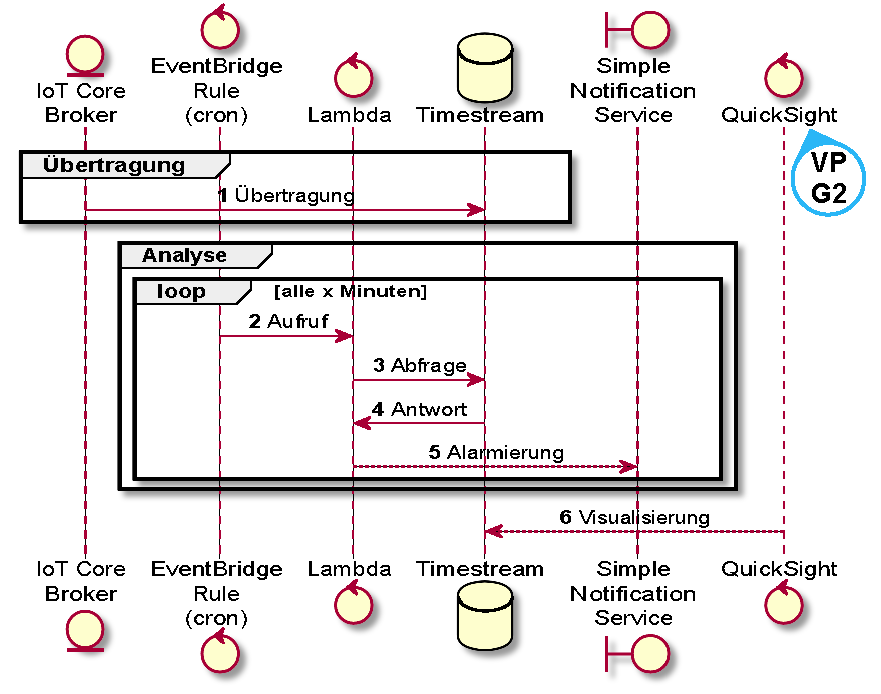
\includegraphics[width=\textwidth]{graphics/batch-ra.pdf}
\caption{Sequenzdiagramm Batch Verarbeitung}
\label{abb:SequenceBatchRA}
\end{figure}



\subsection{Verteilungssicht}
In der folgenden \autoref{abb:TopLevelDBRA} ist die Verteilungssicht der Referenzarchitektur gemeinsam mit den Variationspunkten gezeigt. Variationspunkte mit Präfix G können dabei auch auf bereits definierte Variationspunkte der Echtzeitreferenzarchitektur referenzieren.
\begin{figure}[H]
\centering
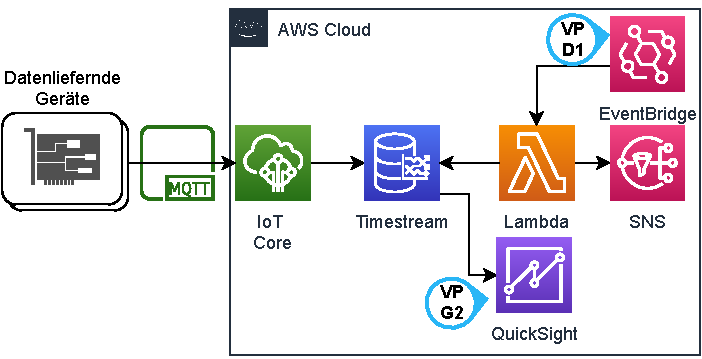
\includegraphics[width=\textwidth]{graphics/DB-RA-Overview.pdf}
\caption{Verteilungssicht}
\label{abb:TopLevelDBRA}
\end{figure}

\vp{D1}: EventBridge bietet den zeitlich geplanten Aufruf von Zielen wie Lambda an. Wenn keine kontinuierliche Überwachung gewünscht ist, kann die Lambda auch auf Bedarf ausgelöst werden. Dies wäre beispielsweise durch ein vorgelagertes API Gateway möglich. Über dieses muss dann der Zeitraum übergeben werden, für welchen die aktuelle Analyse durchgeführt werden soll.

\textbf{Variationspunkt G2:} Hier wird eine Dashboardinglösung, im speziellen der \ac{AWS} eigene Dienst QuickSight vorgesehen. Dies erfolgt, damit Benachrichtigungen, die via \ac{SNS} versendet werden, leicht für die Benachrichtigten nachvollziehbar sind. Wenn also beispielsweise eine Anomalie erkannt wurde, kann dies mit einer Visualisierung nachvollzogen werden, um dann entsprechend zu handeln. Wichtig ist, dass die Visualisierung sowohl von den Originaldaten aus dem Speicher von Timestream gespeist wird, als auch aus der Analyse. Das für und wieder des Einsatzes wurde auch bereits in \vpref{G2} der Echtzeitarchitektur diskutiert. Alternativ ist Timestream auch mit Grafana und damit dem Managed Service von Grafana integriert.\footcite[Vgl.][]{AmazonWebServicesInc..o.J.bm}\nzitat\footcite[Vgl.][]{Dutt.2020} Grafana kann dabei ebenfalls als Dashboardinglösung verwendet werden und kostet dabei das selbe wie die Standard Edition von QuickSight, nämlich 9\$ für Nutzende monatlich.\footcite[Vgl. auch im Foglenden][]{AmazonWebServicesInc..o.J.bn}\nzitat\footcite[Vgl.][]{AmazonWebServicesInc..o.J.bo} Erweiterte Kapazitäten bei QuickSight kosten 18\$ pro Monat für Nutzende. 




\subsection{Bausteinsicht}
In der folgenden \autoref{abb:ElementeDBRA} wird die Bausteinsicht als tiefere Dekomposition der Verteilungssicht, samt Variationspunkten dargestellt.
\begin{figure}[H]
\centering
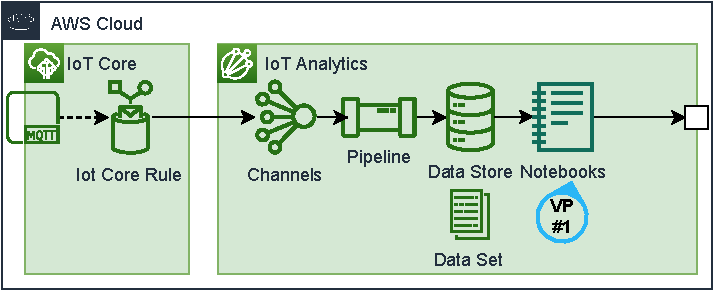
\includegraphics[width=\textwidth]{graphics/DB-RA-Elements.pdf}
\caption{Bausteinsicht}
\label{abb:ElementeDBRA}
\end{figure}

\vp{E1}: Timestream bietet aktuell zwei Speicherklassen an und hat eine Speicherklasse, die für die Zukunft angekündigt ist. Aktuell verfügbar sind \ac{RAM}-basierter Speicher, der teurer ist und magnetischer \ac{HDD}-Speicher, der günstiger ist. Mittels sogenannter \textit{retention policies} können Daten zwischen den Speicherklassen verschoben werden.\footcite[Vgl. auch im Folgenden][]{AmazonWebServicesInc..o.J.bp} Dabei können Daten vom \ac{RAM}-Speicher in den \ac{HDD}-Speicher verschoben werden und vom \ac{HDD}-Speicher gelöscht werden. Beim finalen Löschen der Daten sind die jeweiligen Anforderungen an Datenaufbewahrung der instanziierenden Architektur zu beachten. So können beispielsweise Langzeitanalysen notwendig sein, die auf einen Datenbestand von mehreren Monaten oder Jahren zugreifen müssen. Da Timestream aber auch nach Speicher abgerechnet wird, sind \textit{retention policies} sowohl von \ac{RAM} zu \ac{HDD} als auch zur Löschung von Inhalt vom \ac{HDD}-Speicher einzurichten. Zu beachten ist, dass die Gesamtaufbewahrungsdauer sich aus der Summe beider Aufbewahrungszeiten ergibt. Die Einstellung der \ac{RAM} zu \ac{HDD} retention policy ist abhängig von \vpref{E2} und \vpref{E5}, da je nach Abfragerhythmus und abgefragter Datenmenge für Analysen eine verlängerte Aufbewahrung im \ac{RAM} zur beschleunigten Analyse sinnvoll ist. Für die \ac{SQL}-Abfragen wird kein Unterschied zwischen Speicherart gemacht, bis auf die technisch bedingte höhere Ausführungsdauer auf \ac{HDD}-Speichern.

\vp{E2}: \ac{SQL}-Abfragen in Timestream sind auf mehrere Arten optimierbar. Zum einen wird die abgefragte Datenmenge in Rechnung gestellt, was eine präzise Einschränkung der Abfrage mit \mintinline[breaklines]{sql}{WHERE} Bedingungen und einem genauen \mintinline[breaklines]{sql}{SELECT} notwendig macht. Zusätzlich ist die Datenabfrage in zwei Modellen möglich: dem flachen Modell und dem Zeitreihenmodell. \footcite[Vgl. auch im Folgenden][]{AmazonWebServicesInc..o.J.bq} Das flache Modell schreibt, wie in \autoref{tab:flat-timestream} gezeigt, für jeden Messwert eine eigene Zeile. Entsprechend muss der Messwert in der \mintinline[breaklines]{sql}{WHERE} Bedingung spezifiziert werden.

\begin{table}[H]
\centering
\begin{tabular}{|l|l|l|l|l|}
\hline
time & \begin{tabular}[c]{@{}l@{}}Dimension A\\ (Sensorname)\end{tabular} & measure\_name & \begin{tabular}[c]{@{}l@{}}measure\_value\\ ::double\end{tabular} & \begin{tabular}[c]{@{}l@{}}measure\_value\\ ::bigint\end{tabular} \\ \hline
\begin{tabular}[c]{@{}l@{}}2021-05-10\\ 23:59:59\end{tabular} & sensora & co2 & null & 500 \\ \hline
\begin{tabular}[c]{@{}l@{}}2021-05-10\\ 23:59:59\end{tabular} & sensorb & temperature & 25.5 & null \\ \hline
\end{tabular}
\caption{Beispiel flaches Datenabrufmodell}
\label{tab:flat-timestream}
\end{table}

Gegensätzlich dazu gibt das Zeitreihenmodell, welches sich beispielsweise mit der \\ \mintinline[breaklines]{sql}{CREATE_TIME_SERIES} Funktion erzeugen lässt, \ac{JSON} Arrays zurück. Diese sehen wie folgt aus: \mintinline[breaklines]{json}{[{"time":"2021-05-10 23:59:59","value":500}]}. Timestream bietet für diese Zeitreihen spezielle Funktionen, wie beispielsweise die Interpolation fehlender Werte an.



\vp{E3}: Der Programmcode und die Laufzeit der Lambdafunktion in diesem Variationspunkt sind je nach Anforderungen und Kentnissen des Implementierungsteams bei der Instanziierung dieser Referenzarchitektur anzupassen/neu zu schreiben. In \anhangref{anhang:batch-codesample} ist beispielhaft eine Lambdafunktion, geschrieben in Javascript für die Node.js Laufzeitumgebung, gezeigt. Diese Lambdafunktion sendet eine \ac{SQL}-Abfrage zur Zählung von schwellwertüberschreitenden Werten einzelner Sensoren. Folgend werden die Ergebnisse ausgewertet und für jeden Sensor mit überschreitenden Messwerten eine Benachrichtigung via SNS und ein \textit{shutdown}-Befehl an den Sensor via \ac{MQTT} versendet. Zu beachten ist, dass Lambdafunktionen einen Timeout von 15 Minuten haben..\footcite[Vgl.][]{AmazonWebServicesInc..o.J.bv} Sollten besonders aufwändige Auswertungen durch die Lambdafunktion durchgeführt werden, sollte sie in ein Orchestrierungsdienst wie Step Functions eingebunden werden. Step Functions kann Aufgaben wie automatische Neuversuche oder Fortsetzung der Abfrage durch Übergabe der Abfrage-ID von Timestream erledigen.

\vp{E4}: Unabhängig von dem in \vpref{G2} gewählten Dienst ist es möglich, individuelle Dashboards mit unterschiedlichen Interaktionsmöglichkeiten zu erstellen. So können beispielsweise sogenannte \textit{drill-downs} den Nutzenden Entscheidungsträgern helfen, dynamisch die Datenbereiche anzupassen. Ein Dashboard in QuickSight kann beispielsweise wie folgt aussehen:
\begin{figure}[H]
\centering
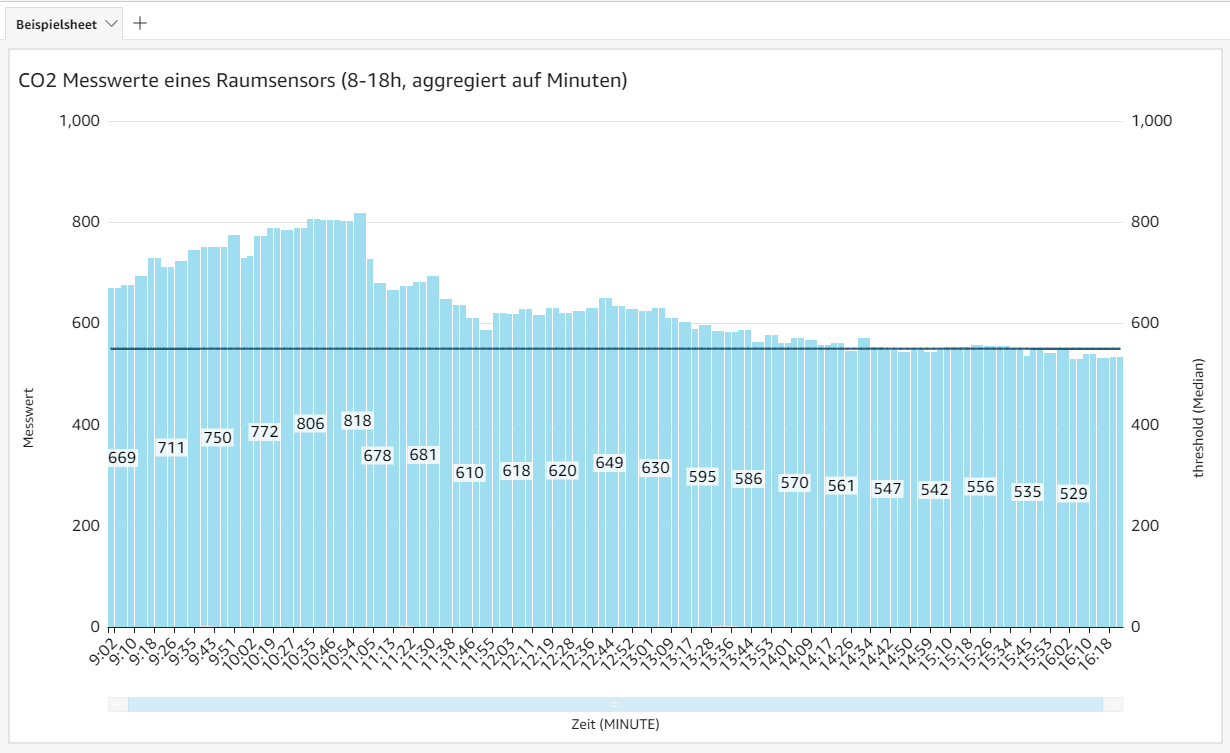
\includegraphics[width=\textwidth]{graphics/QuickSight-Beispiel.png}
\caption{Dashboard in QuickSight}
\label{abb:DashboardDBRA}
\end{figure}


\vp{E5}: EventBridge Regeln können unterschiedlich eingestellt werden. Abhängig von den Anforderungen der instanziierenden Architektur, kann entweder ein Aufruf alle x Minuten, Stunden oder Tage eingestellt werden, oder für mehr Anpassung eine Rate mittels einer abgewandelten, \textit{cron}-Syntax konfiguriert werden. Ein cron-Ausdruck, um die Regel alle 10 Minuten an Werktagen zwischen 9 und 17.00 Uhr auszulösen, sähe wie folgt aus: \mintinline[breaklines]{bash}{0/10 9-17 ? * MON-FRI *}. Der Ausdruck wird in \ac{UTC}-Zeit ausgeführt, was eine ein- oder zweistündige Verschiebung von der deutschen Zeit bedeutet.

\textbf{Variationspunkt G5}: Dieser Variationspunkt ist in der Bedeutung identisch zum \vpref{G5} der Echtzeitreferenzarchitektur.

\TodoW{Networking}

\subsection{Anforderungen}
Folgend wird für die Batch Architektur dargestellt, wie die einzelnen Anforderungen mittels der Referenzarchitektur addressierbar sind.
\subsubsection{Anwendbarkeit auf Monitoringdaten (IT)}
Timestream unterstüzt wie die Kinesis Familie diverse Zeitreihendaten. Es ist ebenfalls prinzipiell möglich Logdaten aufzubewahren, da der interne Datentyp \textit{varchar} Strings mit bis zu 2 GB Länge erlaubt.\footcite[Vgl.][]{AmazonWebServicesInc..o.J.br} Da aber große Datenmengen in einzelnen Variablen durch die doppelten Kosten für Speicherung und Abfrage sich weniger eignen als beispielsweise numerische Messwerte, sollte auf die Anwendung auf Logs verzichtet werden.

Die Nutzung zur Speicherung von Metriken hingegen ist explizit im Rahmen von \textit{DevOps}-Anwendungsfällen für Timestream vorgesehen.\footcite[Vgl.][]{AmazonWebServicesInc..o.J.ak}\nzitat\footcite[Vgl.][]{Das.2020} Ohne spezialisierte Applikation, die beispielsweise in Kinesis Data Analytics mit Flink Laufzeitumgebung laufen könnte und von Kinesis Data Firehose gespeist wird, ist es jedoch nicht möglich CloudWatch Metriken in Timestream zu laden.\footcite[Vgl.][]{Riddle.2021} Alternativ können Metriken wie von \citeauthor{Pochiraju.2020} vorgeschlagen, über \ac{MQTT} und \AWSIOT{} Core in Timestream eingespeist werden.\footcite[Vgl.][]{Pochiraju.2020} Das eine eigene Applikation verwendet werden muss, um Daten via Kinesis oder \ac{MQTT} einzuspeisen, wertet die Tauglichkeit für Monitoring-Usecases gegenüber der Echtzeitarchitektur ab.


\subsubsection{Anwendbarkeit auf Sensordaten (IoT)}
Durch die native Integration mit \AWSIOT{} Core ist eine Integration mit Datensätzen von Sensoren, die via \ac{MQTT} übermittelt wurden vollständig verwaltet möglich. Metadaten der Sensoren können zur Attributierung bei der Auswertung mittels der Dimensionen übermittelt werden, Messwerte als eben solche. Die Menge an Erkenntnissen, die sich aus der Analyse der Sensordaten in Timestream gewinnen lassen, ist wesentlich von \vpref{E5} und damit der Analysefrequenz abhängig.

\subsubsection{Handling von Events, Messwerten und \enquote{Streaming}}
Timestream ist vollständig verwaltet und es sind keine Infrastrukturkomponenten zur Skalierung anzupassen. Da laut Aussage von \ac{AWS} mit dem Dienst Billionen Datenpunkte pro Tag nahe der Echtzeit verarbeitet und abgefragt werden können, ist zu erwarten, dass auch hochfrequente Datenreihen in angemessener Zeit gespeichert werden können.\footcite[Vgl.][]{AmazonWebServicesInc..2020g} Dabei wäre es, wenn die Dateneingangslogik selbst zu schreiben wäre möglich, dass wiederholbare Fehler auftreten. Da aber die Daten automatisiert nach dem Eingang im \ac{MQTT} Broker \AWSIOT{} Core in Timestream gespeichert werden, ist dies nicht nötig. Ein mögliches Problem gibt es maximal bei der Überttragungslatenz zwischen \AWSIOT{} Core und Timestream, auf die kein Einfluss genommen werden kann.
Da Timestream abseits der numerischen Datentypen auch Datentypen vie \textit{varchar} anbietet, ist es möglich auch Events in Timestream abzuspeichern.\footcite[Vgl.][]{AmazonWebServicesInc..o.J.r}


\subsubsection{Automatisierte operative Entscheidungen}
Das Codebeispiel in \anhangref{anhang:batch-codesample} demonstriert, dass es möglich ist, basierend auf den Ergebnissen einer Abfrage automatisiert Abfragen durchzuführen. Dabei zu beachten ist jedoch, dass durch die Intervallverzögerung Aktionen im schlechtesten Fall nach genau $t$ Minuten, nach dem Ereignis ausgelöst werden. Dabei ist $t$ das Intervall zwischen einzelnen Ausführungen, wie beschrieben in \vpref{E5}. Dies kann bei kritischen Aktionen, die möglichst schnell ausgeführt werden sollen jedoch die akzeptable Raktionszeit stark überschreiten. Sollte Timestream ähnlich zu Amazons DynamoDB integrierte Streams als Feature bekommen, welche Änderungen am Datensatz zur Verarbeitung an Plattformen wie Lambda senden, wäre dieses Problem addressierbar.

\subsection{Produktives Monitoringkonzept}
In \autoref{tab:cloudwatch-metrics-db} sind die zu überwachenden Cloud-Watch Metriken der in der Referenzarchitektur verwendeten Dienste gezeigt. Dies umfasst TimeStream, Lambda, \ac{SNS}, \AWSIOT{} Core und EventBridge.\footcite[Vgl.][]{AmazonWebServicesInc..o.J.be}\nzitat\footcite[Vgl.][]{AmazonWebServicesInc..o.J.bf}\nzitat\footcite[Vgl.][]{AmazonWebServicesInc..o.J.bc}\nzitat\footcite[Vgl.][]{AmazonWebServicesInc..o.J.az}\nzitat\footcite[Vgl.][]{AmazonWebServicesInc..o.J.bl}


\begin{table}[H]
\centering
\begin{tabular}{|l|l|l|l|}
\hline
Dienst & Metrik & Ursache & Detektionsart \\ \hline
\rowcolor[HTML]{F5F5F5} 
\ac{SNS} & NumberOfNotificationsFailed & Dienstfehler & Schwellwert \\ \hline

\multirow{2}{*}{\AWSIOT{} Core} & RuleMessageThrottled & \begin{tabular}[c]{@{}l@{}}Dienstfehler/\\ Benutzungsfehler\end{tabular} & Schwellwert \\ \cline{2-4} 
 & Failure & \begin{tabular}[c]{@{}l@{}}Dienstfehler/\\ Benutzungsfehler\end{tabular} & Schwellwert \\ \hline
 
\rowcolor[HTML]{F5F5F5} 
\cellcolor[HTML]{F5F5F5} & SystemErrors & Dienstfehler & Schwellwert \\ \cline{2-4} 
\rowcolor[HTML]{F5F5F5} 
\cellcolor[HTML]{F5F5F5} & UserErrors & Benutzungsfehler & Schwellwert \\ \cline{2-4} 
\rowcolor[HTML]{F5F5F5} 
\multirow{-3}{*}{\cellcolor[HTML]{F5F5F5}TimeStream} & SuccessfulRequestLatency & \begin{tabular}[c]{@{}l@{}}Dienstfehler/\\ Benutzungsfehler\end{tabular} & Anomalie \\ \hline

\multirow{3}{*}{Lambda} & Duration & \begin{tabular}[c]{@{}l@{}}Dienstfehler/\\ Benutzungsfehler\end{tabular} & Anomalie \\ \cline{2-4} 
 & Errors & \begin{tabular}[c]{@{}l@{}}Dienstfehler/\\ Benutzungsfehler\end{tabular} & Schwellwert \\ \cline{2-4} 
 & Throttles & Benutzungsfehler & Schwellwert \\ \hline
 
\rowcolor[HTML]{F5F5F5} 
\cellcolor[HTML]{F5F5F5} & FailedInvocations & Dienstfehler & Anomalie \\ \cline{2-4} 
\rowcolor[HTML]{F5F5F5} 
\multirow{-2}{*}{EventBridge} & ThrottledRules & Dienstfehler & Schwellwert \\ \hline
\end{tabular}
\caption{CloudWatch Metriken}
\label{tab:cloudwatch-metrics-db}
\end{table}

\AWSIOT{} Core, \ac{SNS} und Timestream übermittelt Metriken in einminütiger Auflösung.\footcite[Vgl.][]{AmazonWebServicesInc..o.J.az}\nzitat\footcite[Vgl.][]{AmazonWebServicesInc..2021b}\nzitat\footcite[Vgl.][]{AmazonWebServicesInc..o.J.be} 
Bei Lambda können die übermittelten Metriken bis nach Ende einer Ausführung übermittelt werden, weshalb die Auflösung der Metriken unpräzise sein kann. Insgesamt lässt sich aufgrund der teilweise verketteten Metriken leicht erkennen, wenn kaskadierende Fehler auftreten. So sind beispielsweise \textit{FailedInvocations} von EventBridge ein Hinweis darauf, dass es Probleme bei der Ausführung von Lambda Funktionen gab.



\subsection{Know-how für instanziierende Architekturen}
Während Timestream zum Start 2020 allein in Irland (eu-west-1) für die EU verfügbar war, ist Timestream für die Region eu-central-1 (Frankfurt) mittlerweile verfügbar.\footcite[Vgl.][]{AmazonWebServicesInc..2020g}\nzitat\footcite[Vgl.][]{AmazonWebServicesInc..o.J.q} Dies erleichtert die Integration in bestehende Dienste, die bereits in Frankfurt provisioniert wurden.

Zeitreihen mit Messwerten und Metadaten werden innerhalb von Timestream als Dimensionen oder Messwerte hinterlegt. Dimensionen und Messwerte haben jeweils einen Namen und einen Wert. Dabei sind als Dimensionen alle Metadaten des übermittelnden Sensors oder der übermittelnden Applikation denkbar. Beispiele für solche Dimensionen wären Name oder Standort, während Messwerte beispielsweise \coo{} Messungen, Temperaturen, CPU Auslastung oder \ac{RAM}-Verbrauch sein können. Timestream rechnet pro Schreibzugriff die Summe aller Namen von Dimensionen und Messwerten und deren Werte (inklusive der Zeitdimension mit aktuellem Zeitstempel) als Speicherplatz ab.\footcite[Vgl. auch im Folgenden][]{AmazonWebServicesInc..o.J.bs} Bei gruppierten Schreibzugriffen können gemeinsame Attribute und Werte zusammengefasst werden, um die Anzahl an Schreibzugriffen zu vermindern.
Aus der Unterteilung in Messwerte und Dimensionen ergeben sich auch Optimierungen der Datenmodellierung. So gibt es beispielsweise die Möglichkeit, derivative Werte, sofern sie eine niedrige Kardinalität besitzen als Dimensionen statt als Messwerte zu speichern.\footcite[Vgl. auch im Folgenden][]{AmazonWebServicesInc..o.J.bt} Dies bringt aber den Nachteil mit sich, dass entsprechend drei verschiedene Zeitreihen entstehen würden, was bei der Abfrage zu beachten ist. Da Dimensionsnamen ebenfalls Speicherplatz verbrauchen, sind die Namen entsprechend des Ockhams Rasiermesser zu gestalten und die einfachste und kürzeste Variante auszuwählen. Bei der Datenmodellierung ist auch zu beachten, dass Messwerte entsprechend ihres eigentlichen Datentyps gespeichert werden und keine unbeabsichtigte Konversion in z.B. das \textit{varchar} Format auftritt. Da Messwerte bei Erstanlage eines Messwertes in einer Tabelle fest mit einem Datentypen assoziiert werden, ist eine Neuanlage mit entsprechender Datenmigration notwendig um Fehler zu korrigieren.





\section{Einsatzszenarien der Referenzarchitekturen}
Ob die Referenzarchitekturen im Tagesgeschäft eingesetzt werden können, soll anhand der Qualitätskriterien für Referenzarchitekturen überprüft werden. Aus diesem Grund wurden in  \anhangref{anhang:interview-philipp-03.05.2021}, \anhangref{anhang:interview-viet-04.05.2021} und \anhangref{anhang:interview-jan-04.05.2021} Interviews mit diversen Stakeholdern der Cloud Entwicklung geführt. Dabei war eine Verständlichkeit trotz der unterschiedlichen technischen Hintergründe der Interviewpartner zu erkennen. Ebenfalls haben die Stakeholder die Referenzarchitekturen akzeptiert und sahen die Qualität als zufriedenstellend an. Aufgrund des Feedbacks aus \anhangref{anhang:interview-viet-04.05.2021} wurden zwischen dem Stand zur Zeit des Interviews und dem finalen Stand Diagramme in mehrere aufgeteilt. Dies dient auch der Behebung des Zuordnungsproblems aus \anhangref{anhang:interview-jan-04.05.2021}.

Eine Zugänglichkeit und ein Zugriff durch die Mehrheit der Organisation ist auf zweierlei Arten sichergestellt: Zum einen wird die fertige Bachelorarbeit an mehreren Stellen in den internen Wissensmanagementsystemen wie Confluence publiziert und zum anderen ist die Bachelorarbeit auf GitHub open source verfügbar.\footnote{Siehe \url{https://github.com/LukvonStrom/Bachelorarbeit}} Eine Wartbarkeit ist durch den offenen Prozess des Forkens via dem Versionsverwaltungstool Git und der offenen MIT-Lizenz, wie auch in \anhangref{anhang:interview-philipp-03.05.2021} erläutert, gewährt. Die Hauptprobleme dieser Domäne sind insofern adressiert, dass die Referenzarchitekturen mit den $\kappa$ und \ac{OLAP} Patterns auf etablierten Mustern basieren. Wertschöpfung für den Betrieb ist insofern garantiert, dass der Bedarf der Behandlung des Themas aus dem Geschäftsalltag entstanden ist, wie in \anhangref{anhang:interview-philipp-03.05.2021} erläutert.


Im Folgenden soll beleuchtet werden, wofür sich welche der beiden entwickelten Referenzarchitekturen besser eignet.
Für das Monitoring eignet sich die in \autoref{chap:ra-rt} beschriebene Referenzarchitektur besser, da eine enge Integration sowohl mit CloudWatch Metrics als auch CloudWatch Logs besteht. So lassen sich Analysen zu in der \ac{AWS}-Cloud laufenden Workloads einfach durchführen. Dadurch, dass keine eigene Software geschrieben werden muss, um die Metriken in das Analysesystem zu laden, ist dieser Usecases wesentlich günstiger im Sinne des firmenseitigen Investments abgedeckt.

Beide Referenzarchitekturen integrieren sich gut mit \AWSIOT{} Core und besitzen damit eine wichtige Voraussetzung zur Analyse der \ac{IoT} Daten. Gemäß der in \autoref{chap:datenwert} erläuterten Datenhalbwertszeit ist eine Auswahlentscheidung auch in Abhängigkeit von den Analyseanforderungen der Share- und Stakeholder der instanziierenden Architektur zu treffen. Unter Einsatz einer Dashboardinglösung wie QuickSight oder Grafana können historische Daten bei beiden Referenzarchitekturen auch Entscheidern zugänglich gemacht werden, wenn die Datenablage in \ac{S3} erfolgt. 

Sollten längere Aufbewahrungsfristen der Daten über 30 Tage hinaus gewünscht sein, ist die Batch Architektur zu empfehlen, da die Datenhaltung großer Mengen an historischen Daten zu Analysezwecken möglich ist. Alternativ könnten beide Architekturen auch, ähnlich zur $\lambda$-Architektur kombiniert werden, um Timestream als Aufbewahrungslösung für ältere Daten bei Bedarf zu verwenden und Analysen über Echtzeitdaten mittels Kinesis durchzuführen. Bei einer solchen Kombination wäre zu beachten, die Speicherklasse \ac{HDD} zu verwenden, da die Latenz von Abfragen dann weniger kritisch ist. Wenn eine intervallbasierte Auswertung tolerierbar ist, ist Timestream zu verwenden, da die Gesamtkosten abhängig von der Art der Abfragen und die Komplexität der Architektur niedriger sind, als bei der Echtzeitreferenzarchitektur.


Da die Referenzarchitekturen als verteilte Systeme mit mehreren Diensten diverse Fehlerquellen haben können, die sich dann symptomatisch in den gezeigten Metriken bemerkbar machen, sind genaue Tests zum Verständnis der Fehlerzustände wichtig. Im Rahmen des \textit{Chaos Engineerings} lassen sich gezielt Fehler in das System einführen um die Resilienz gegenüber diversester Fehlerquellen zu testen.\footcite[Vgl.][]{Augsten.2020} Bei den vorgestellten Referenzarchitekturen ist es zu empfehlen, regelmäßige Chaos Experimente durchzuführen um gezielt Fehlerszenarien wie doppelte Nachrichten, hohe Latenzen zwischen Diensten oder die temporäre Nichtverfügbarkeit einzelner Dienste zu simulieren und gezielt den Einfluss messen zu können. Folgend können Erkentnisse für den besseren Betrieb einer resilienten Dateninfrastruktur abgeleitet und dokumentiert werden. Für \ac{AWS} gibt es den Dienst Fault Injection Simulator, welcher Fehler in Schnittstellen zwischen Diensten erzeugen kann und gezielt auch einzelne Infrastrukturkomponenten beeinträchtigen kann.\footcite[Vgl.][]{Barr.2021b} Unter Verwendung dieses Dienstes ist es möglich, die beschriebenen Chaos Experimente durchzuführen.

In den vorliegenden Referenzarchitekturen wurde gemäß \autoref{abb:DimensionenUebersicht} eine \enquote{so tief wie notwendige} Dekomposition erreicht, indem Variationspunkte mit starken Auswirkungen in stärkerer Detailtiefe erklärt werden, während beide Referenzarchitekturen auf den selben Dekompositionssichten aufbauen.

Eine hohe Anwendbarkeit wurde von den diversen Stakeholdern wie oben beschrieben in \anhangref{anhang:interview-philipp-03.05.2021}, \anhangref{anhang:interview-viet-04.05.2021} und \anhangref{anhang:interview-jan-04.05.2021} attestiert.
In Sachen Allgemeingültigkeit wurde insofern ein leicht abgesenkter Standard erreicht, da sich aufgrund der Prioritäten des Dienstvergleiches, die durch wichtige Stakeholder durchgeführt wurden eine für die Zielorganisation spezifische Architektur ergeben hat. Andere Organisationen, die beispielsweise eine Übertragbarkeit zwischen Clouds als wichtiger empfinden, hätten möglicherweise alternative Dienste wie OpenSearch in der Batchverarbeitung gewählt, aufgrund eines anders priorisierten Vergleiches.


\chapter{Schlussbetrachtung}\label{chapter:Schlussbetrachtun}
Folgend sollen die Ergebnisse der Arbeit zusammengefasst und kritisch reflektiert werden. Anschliessend wird ein Ausblick gegeben.
\section{Zusammenfassung}\label{section:Zusammenfassun}
Das Ziel dieser Arbeit bestand darin, die gängigen Dienste im \ac{AWS} Umfeld zur Zeitreihenverarbeitung zu evaluieren und folgend Referenzarchitekturen zu konstruieren. Mittels mehrerer Interviews wurden Anforderungen an die Referenzarchitekturen und deren Gestaltung erhoben, welche später in den Konstruktionsprozess eingeflossen sind. 
Für die spätere Konstruktion wurden bekannte Architekturmuster mittels Literaturrecherche dargestellt. Theoretische Grundlagen zum Wert von Daten über die Zeit und zur Konstruktion von Referenzarchitekturen, inklusive der Systematik der Variationspunkte, wurden mittels Literaturrecherche dargestellt. Nach einer Darstellung von bereits existierenden Anwendungsfällen, wurden durch eine Umfrage die Kriterien für den folgenden Dienstvergleich priorisiert. Anschließend wurde ein Dienstvergleich für die relevanten Dienste von \ac{AWS} durchgeführt.

Nach durchgeführtem Dienstvergleich konnten mit den Resultaten zwei Referenzarchitekturen für Echtzeit- und Batchverarbeitung von Zeitreihendaten konstruiert und in verschiedenen Dekompositionssichten dargestellt werden.

Dank weiteren Gesprächen mit diversen Stakeholdern wurde festgestellt, dass die Referenzarchitekturen nutzenstiftend sind und künftig zum Einsatz kommen.

Mittels der open-source vorliegenden Referenzarchitekturen können künftig interne Usecases und Kundenusecases im Bereich Zeitreihenverarbeitung in \ac{AWS} leichter umgesetzt werden, da es ab sofort eine klar definierte Referenzarchitektur mit definierten Variationspunkten gibt.


\section{Kritische Reflexion}\label{section:Kritische-Reflexio}
Innerhalb dieser Arbeit wurden Referenzarchitekturen für die Verarbeitung in der Cloud konstruiert. Ein Trend der dabei ausgespart wurde, weil sich wichtige Komponenten nicht in der Cloud befinden, ist das sogenannte \textit{Fog computing}. Nach der Definition von \citeauthor{Vaquero.2014} ist Fog computing ein Szenario, in dem heterogene, allgegenwärtige und dezentralisierte Geräte kommunizieren und kooperieren um Speicher- und Verarbeitungsaufgaben zu übernehmen.\footcite[Vgl.][30\psq]{Vaquero.2014} In der Praxis führt dies dazu, dass Verarbeitungsaufgaben in Teilen, angelehnt an das \textit{Edge computing} von der Cloud in Richtung der Geräte ausgelagert wird.\footcite[Vgl.][]{Bonomi.2012} Dies geschieht dabei beispielsweise an Netzwerkgateways, die sowieso mit der Cloud kommunizieren und folgend nur noch bereits ausgewertete Daten übertragen. 

Im Rahmen der konstruierten Monitoringkonzepte fehlen konkrete Maßnahmen, die im Falle einer Fehlermeldung auszuführen sind. Dies resultiert aus dem reaktiven Incident-response Ansatz, den die SPIRIT/21 im Bezug auf Incidents mit \ac{AWS}-nativer Infrastruktur durchführt.

Im Rahmen der Anforderungserhebung wurden mit den diversen Stakeholdern Interviews geführt. Bei diesen schien die Verständlichkeit der vorab zugesendeten Materialien nicht vollständig gegeben zu sein. Aus diesem Grund musste den Stakeholder teilweise erklärt werden, wie die Kriterien konkret zu verstehen sind, damit diese eine Bewertung vornehmen konnten. Dies hätte womöglich durch die Bereitstellung von mehr Kontext bereits vor den Interviews verhindert werden können.

Obwohl die Referenzarchitekturen in den wesentlichen Punkten mit den Vorschlägen des \ac{AWS} Well-Architected Frameworks (bzw. im spezifischen der Analytics Lens) übereinstimmen, wurden die Architekturen nicht an den Kriterien final gemessen. Dies liegt auch mit der Ambiguität von Kriterien wie \textit{Orchestrate ETL workflows} zusammen, bei denen die Erfüllung schwer gemessen werden kann.\footcite[Vgl.][6]{Ravirala.2020}

Aufgrund des hohen Bezuges auf \ac{AWS} Technologien und Dienste musste mit einigen Quellen gearbeitet werden, die von \ac{AWS} verfasst wurden oder von Personen, die mit \ac{AWS} affiliiert sind oder waren. Wo möglich und verfügbar wurden kritische Positionen eingebunden.


\section{Ausblick}\label{section:Ausblic}
\ac{AWS} bietet mit dem Dienst Greengrass bereits eine Softwareplattform an, die auf diversen qualifizierten Gateways läuft.\footcite[Vgl. auch im Folgenden][]{AmazonWebServicesInc..o.J.bu} Durch die lokale Ausführung von Code könnten Schwachstellen adressiert werden, wie beispielsweise schlechte Netzkonnektivität. So kann Code, der auf Greengrass ausgeführt wird in Form von Containern oder lokalen Lambdafunktionen Benachrichtigungen lokal ohne Konnektivität zur Cloud versenden und beispielsweise Aktoren auslösen. Dies würde die gezeigten Referenzarchitekturen ergänzen. Das dies mit Greengrass Anomaliedetektion möglich ist, wurde auch von \citeauthor{Shankar.2020} gezeigt.\footcite[Vgl.][]{Shankar.2020}

Anschließend zur Abgabe der Bachelorarbeit wird das GitHub Repository mit dem Quelltext der Bachelorarbeit veröffentlicht. Zusätzlich werden die Referenzarchitekturen an mehreren internen Stellen wie dem internen Wissensmanagement Confluence abgelegt, um einfache Zugänglichkeit zu gewährleisten.

Nach Fertigstellung der Arbeit ist vorgesehen, die Referenzarchitekturen mittels dem \ac{AWS} \ac{CDK}, der \ac{AWS}-nativen \ac{IaC} Lösung umzusetzen. Dies erlaubt automatisches Ausrollen aller beteiligten Infrastrukturkomponenten. So ist die Wiederverwendbarkeit über die reinen Architekturmuster hinaus möglich, da allein der Code der beteiligten Ressourcen angepasst werden muss.

Wie auch in \anhangref{anhang:interview-viet-04.05.2021} bestätigt, werden die Referenzarchitekturen in künftigen Kunden-Usecases genutzt. Damit kann sich der Nutzen für die Native Cloud Solution der SPIRIT/21 auch in der Praxis zeigen.



\chapter*{Anhang}
\addcontentsline{toc}{chapter}{Anhang}
\section*{Anhangverzeichnis}
\vspace{-8em}

% vor \listofanhang müssen Einrückungen angepasst werden
\abstaendeanhangverzeichnis

\listofanhang
\clearpage
\spezialkopfzeile{Anhang} % damit in der Kopfzeile das Wort "Anhang" angezeigt wird

% \anhang{So funktioniert's}

% \lstset{language=TeX, % hervorzuhebende Keywords definieren
%   morekeywords={anhang, anhangteil}
% }


% \anhang{Experteninterviews}
% Im folgenden Anhangteil finden sich die transkribierten Experteninterviews, welche in verschiedenen Phasen der Bachelorarbeit geführt wurden.



\interview{Philip A.}{Cloud Solution Architekt}{NCS}{Initiales Anforderunginterview}{22.03.2021}{philipp}

\newcommand{\LF}{\textbf{Lukas F.:}~}
\newcommand{\PA}{\textbf{Philipp A.:}~}

\LF	Herzlich willkommen zum Interview und vielen Dank, dass du dich als Interviewpartner bereit gestellt hast

\PA	 Selbstverständlich.

\LF	Ich habe direkt eine Frage an dich: Was ist deine Rolle innerhalb der SPIRIT und was ist deine Rolle im spezifischen mit Perspektive auf die Referenzarchitekturen, die es zu entwickeln gilt?

\PA	Ich sitze in der Spirit auf dem Posten des Cloud Solution Architects speziell für \ac{AWS}. Diese Rolle fülle ich auch in der Native Cloud Solution aus. Das heißt, ich bin für Software und Infrastruktur Struktur Architekturen in dem Projekt/der Solution verantwortlich und kümmere mich darum, dass die Implementierung so gut wie möglich voran gehen kann. Dabei sollen keine Architekturprobleme verursacht werden. Ansonsten berate ich die Entwicklung  bei technischen Fragen und Implementierungsfragen, die auftreten.

\LF	Wenn wir jetzt speziell Richtung Referenzarchitektur schauen, würdest du dich dann eher als Nutzenden sehen oder eher als jemand, der zwar einen \enquote{Stake} hat, dass es eine gute der Referenz Architektur wird, aber sie nicht konkret anwenden würde?

\PA	 Ich sehe mich auf beiden Seiten. Sowohl als Nutzenden, weil ich werde auf Basis der Referenzarchitekturen unsere Serverless Solutions designen, also die für uns und unsere Kunden. Ich glaube aber auf der anderen Seite auch, dass ich mitwirke an der Ausarbeitung.

\LF	 Verstehe, das ist schon mal aufschlussreich. Insgesamt, wir reden ja über Referenzarchitekturen, wo siehst du denn Anwendungsgebiete? Gibt es konkrete Customer Cases, wo wir jetzt auf Zeitreihendaten speziell schauen, oder gibt es da irgendwelche Gebiete, wo du sagst: \enquote{Oh, da könnte es besonders relevant sein}?

\PA	 Ja natürlich. Der größte/aktuellste Fall bei uns sind tatsächlich Sensordaten und Messdaten im \ac{IIoT} Umfeld, bei denen wir solche Zeitreihendaten immer haben. Aber auch sämtliche Monitoring Daten, die von cloudbasierten Metriken abgezogen werden. Von diesen Metriken gibt es viele.

\LF	So wie ich es verstehe, sowohl interne Anwendungsfälle mit Monitoring als auch Sachen, die für Kunden jetzt direkt relevant sind, wie \ac{IIoT}-/Sensordaten

\PA	 genau

\LF	 Das wären denke ich so die Bereiche, in denen man die Referenz Architekturen anwenden würde/ spezialisieren würde.

\PA	 Da wir uns, in der SPIRIT eben auch mit Applikation Management befassen, ist es eben auch ein internes Thema. Wir wollen selber sehen, wie wir möglichst effizient Architekturen zum Betrieb, also auch zum Monitoring aufbauen können. Gleichzeitig ist es auch ein Kundenthema, weil wir öfters Anfragen kriegen zum Thema \ac{IIoT} Umsetzung/ \ac{IIoT}-Implementierung und deren Folgen, die Auswirkung der Daten.

\LF	Insgesamt, wenn wir an Referenzarchitekturen denken, ich rede davon gleich mal im Plural, weil es aus meiner Sicht schon mal mindestens zwei geben muss, als Artefakt meiner Bachelorarbeit. Wie kompatibel sollen die denn zueinander sein, wenn wir uns vorstellen, es gibt zum Beispiel eine für die Echtzeit Verarbeitung und eine für die Batch-Verarbeitung von Daten? Müssen die austauschbar sein, also von derselben Quelle zum Beispiel \enquote{gefüttert} werden? Oder ist es da okay jeweils recht spezifische Pipelines zu bauen, die  dann programmatisch eingebunden werden müssen, relativ nah am Datenerzeugenden?

\PA	 Ich finde, das ist eine Frage, die die Arbeit beantworten sollte, denn ich kann das aus meiner aktuellen Position schwer abschätzen. Für mich ist es nicht klar, ob es sinnvoller ist individuell, also wenn man dem Erzeuger nahestehend die Daten dort auf ein Format zu bringen, die sich laden lassen, oder ob es sinnvoller ist, die Daten vom Erzeuger zu nehmen und dann in der Referenzarchitektur zu normalisieren und anzugleichen.

\LF	 Ich hatte jetzt nicht unbedingt an Daten direkt gedacht, sondern mehr an die Infrastruktur, die kompatibel sein muss. So dass es am Anfang eine Schnittstelle zum Beispiel geben würde, was eine Art Plug and Play mit beiden Ansätzen ermöglichen würde oder einfach das nur einen Ansatz quasi mit mit einer Customization sozusagen funktioniert?

\PA	Ach so. Zu wünschen wäre es natürlich, wenn wir hinterher nur eine Hauptarchitektur hätten oder möglichst wenig Anpassungen an die Architekturen vornehmen müssen, um die Sachen zu switchen. Das ist natürlich aus der Architektenbrille die schönere Sache. Auf der anderen Seite glaube ich tatsächlich, wenn man sich einmal festgelegt hat auf eine von beiden Arten, dass man dann eh nicht mehr switchen wird. \\
Da muss man sich eben vorher klar werden, welchen Weg man gehen will. Es ist eigentlich völlig valide zu sagen, wenn ich weiß, dass ich Batch Verarbeitung mache, dann habe ich auch genau diese Architektur. Die Anforderung, dass man wechseln muss, ist zu vernachlässigen. Interessanter ist es eher, wenn man sagt ich brauche beides. Womöglich lohnt es sich da, beides zu inkludieren.

\LF	 Zu meiner nächsten Frage: Ich habe dir im Vorfeld zwei Listen zugesendet, wo ich gerne deine Meinung hören würde, wie du die jeweils priorisieren würdest. Zum einen sind das die Qualitätskriterien von Referenzarchitekturen und zum anderen die datenbezogenen Entscheidertypen. Fangen wir am besten mit den Qualitätskriterien an.

\PA	 Genau

\LF	Da hat es ja sieben. Welche würdest du denn relativ weit oben aus deiner Position raus positionieren? Und welche sind von eher nachrangiger Relevanz?

\PA	Ich picke von den sieben mal drei raus und vielleicht kannst du mir zu dem einen oder anderen Punkt noch ein bisschen was erläutern. Der Punkt fünf \enquote{akzeptabel}, da verstehe ich nicht so wirklich, was du damit meinst. Beim  Thema \enquote{wertschöpfend für den Betrieb} versteh ich jetzt auch nicht so, was du damit meinst im Vergleich zur Adressierung der Hauptprobleme. Kannst du das nochmal kurz erläutern?

\LF	\enquote{Wertschöpfend für den Betrieb}: So wie ich den Autor verstehe, mein das, das man einen Wert daraus hat, die Referenzarchitekturen anzuwenden und es sich nicht lohnt von \enquote{scratch} anzufangen.

\PA	 Okay. Wie sieht es mit akzeptabel aus?

\LF	Beim Kriterium \enquote{akzeptabel} verstehe ich den Autor so, dass man sich als jemand mit Fachkenntnissen im Prinzip das anschaut und sagt ja, das kann ich akzeptieren mit meinen Fachkenntnissen und das ist jetzt nicht völlig an den Haaren herbeigezogen. Es ist quasi \enquote{reasonable}.

\PA	Das ist ja hoffentlich jeder Architektur. Wenn man das nicht mal voraussetzen kann, dann muss man eigentlich Punkt fünf als ersten nehmen es muss natürlich logisch, also \enquote{reasonable} sein. Das nächste muss sein, dass es wertschöpfend ist in irgendeiner Weise, denn man macht nichts, was nicht einen Mehrwert darstellt. Wo ich Schwierigkeiten habe, ist mit \enquote{reasonable}  weil \enquote{Adressierung der Hauptprobleme} hängt natürlich mit dem \enquote{reasonable} zusammen.\\
Damit eine Referenzarchitektur wertschöpfend ist, muss sie aber auch verständlich sein. Jetzt ist die Frage, wie breit Verständlichkeit gehen muss. Hier steht eine breitere, heterogene Gruppe. So weit würde ich jetzt nicht gehen. Aber es muss verständlich sein für diejenigen, die die Referenzarchitektur anwenden müssen und da tatsächlich relativ einfach verständlich. Aber wenn das andere nicht gegeben ist, dass sie \enquote{reasonable} ist, oder das die Probleme der Domäne nicht abgebildet werden, hilft sowieso alles nix.

\LF	 Das heißt du würdest tendenziell, dass es akzeptabel ist und die Probleme adressiert vorne anstellen, gefolgt von der Verständlichkeit?

\PA	 Nein, wertschöpfend ist tatsächlich noch Nummer zwei, vielleicht sogar Nummer eins. Wenn es nicht wertschöpfend ist, dann brauche ich das nicht zu machen, dann habe ich nur Papierkrieg. Es muss einen Mehrwert für den Betrieb geben, das ist eigentlich Nummer eins, unser zweites ist, dass es akzeptabel sein muss, in Kombination mit der Problemlösung der Domäne. Dann kommen wir zu Thema Verständlichkeit.

\LF	 Verstehe. Wenn wir übergehen zu den Datenentscheider- oder -nutzungstypen gibt es ja drei Stück.  Die taktischen, die operativen und die strategischen Entscheider. Wo siehst du denn uns am ehesten? Letztendlich ist das ja die Basis dafür, die wir die Daten analysieren wollen, also in welchen Entscheidungshorizont wir agieren und mit welcher Dringlichkeit wir neue Daten brauchen, um Entscheidungen abzuleiten.

\PA	 Wer ist denn wir? Das hängt natürlich davon ab, was das für Daten sind und was der Ziel der Daten sind, beziehungsweise was das Ziel ist. Ist das Ziel Monitoring, dann habe ich da natürlich erst mal eine sehr kurzfristige Datenlage, die ich bewerten muss. Also wenn beispielsweise der Speicherplatz vollläuft, ist das wichtiger. Wenn ich irgendwelche \ac{IIoT} Daten habe, kann es durchaus sein, dass das eher langfristige Informationen sind. Wenn ich die Temperatur messe oder den \coo{} Gehalt messe, habe ich auch durchaus Interesse an der Langfristigkeit der Daten.

\LF	 Verstehe also tendenziell würdest du, wenn es um Monitoringdaten geht eher dem taktischen Entscheidertyp folgen, der recht früh betrachtet, wenn sich was ändert und seine Entscheidung im Zweifelsfall anpasst. \ac{IIoT} siehst du also eher Richtung operative Entscheider?

\PA	Auch da hängt es wieder von der Art der Daten ab. Wenn es ein \ac{IIoT} Sensor ist, der messen soll, ob es ein Feuer gibt, dann ist es eine taktische Entscheidung, dann den Feueralarm zu betätigen. Wenn es aber Daten sind, die das Wetter beobachten, dann ist es vielleicht interessanter als strategischer Entscheider ranzugehen. \\
Es ist sehr datenbezogen. Beim Monitoring vielleicht ein bisschen weniger. Auch aus Monitoringdaten kann ich natürlich Sachen ziehen, wenn ich nach einem halben Jahr Monitoring sehe, in welchen Intervallen meine Systeme besonders ausgelastet sind. Davon können natürlich auch Entscheidungen abgeleitet werden. Die meisten Informationen beim Monitoring sind aber tatsächlich kurzfristige. Und bei \ac{IIoT} kann ich das kann ich das gar nicht einschätzen, weil da bin ich nicht so tief drin und die Systeme von \ac{IIoT} sind so mannigfaltig. Das ist ja keine Domäne an sich, sondern es ist ja eher eine Infrastruktur, die auf verschiedene Domänen anwendbar ist, je nachdem, was das für Sensordaten sind oder auch in welchen Intervallen die abgefragt werden. Wenn es Sensoren gibt, die jede halbe Stunde Daten melden, dann ist die Echtzeit Entscheidung eher sekundär. Wenn es aber Daten sind, die alle zehn Sekunden anfallen, ist das eher interessanter für Echtzeitentscheidungen.

\LF	 Also du meinst es kommt wesentlich auf die Messdistanz der Sensordaten an?

\PA	 auf jeden Fall

\LF	 Verstehe. Zum zweiten Teil des Interviews: Ich habe ein Dimensionsmodell konstruiert für Referenzarchitekturen, wo es jetzt um die subjektive Allgemeingültigkeit, die Anwendbarkeit, und die Dekompositionstiefe gehen soll. Jetzt wäre meine Frage jeweils, wie du drei Punkte einschätzt auf einer Skala von Null bis fünf und wieso. Wie wichtig ist dir subjektive Allgemeingültigkeit, wie tief muss eine Dekomposition stattfinden, damit Referenz Architekturen gut sind und wie konkret oder abstrakt darf die Referenzarchitektur sein, dass sie nutzenstiftend für viele Anwendungfälle ist, aber trotzdem eingesetzt werden kann.

\PA	 Die Allgemeingültigkeit und die Anwendbarkeit hängen stark vom Teilnehmerkreis ab, also wie groß sehen wir den Teilnehmerkreis der Leute, die mit dieser Referenzarchitektur arbeiten sollen? Je größer der ist, desto größer muss natürlich auch die Allgemeingültigkeit sein. Wenn wir das in dem relativ engen Rahmen sehen, auf Abteilungsebene oder vielleicht bisschen größer, dann können diese beiden Punkte relativ eng gefasst sein. \\
Bei der Dekompositionstiefe , das ist aus meiner Sicht eine Fleißarbeit. Je detaillierter die Dekompositionstiefe ist, desto einfacher ist es vermutlich, die Referenz Architektur in eine echte umzusetzen Architektur. Man hat da ja dann schon viele Hilfestellungen, Beispiele, etc. . Erfahrene Architekten können dann auch die Dekompositionstiefe wählen, die sie brauchen. Die Dekompositionstiefe ist bei der Anwendbarkeit Teil des Kontext. Da ist es eben die Frage, wie groß die Bandbreite ist, wenn wir sagen, wir haben genau diese zwei Usecases, nämlich Monitoring und \ac{IIoT}, dann kann die schon relativ konkret sein. Wenn wir sagen, wir haben vor, das irgendwie über die komplette Organisation und Firma zu stülpen, dann ist es halt sehr abstrakt. Ich halte nicht so viel davon, Dinge zu abstrakt zu machen, weil sie dann tatsächlich oft nicht verstanden werden und auch nicht benutzt werden. Je abstrakter ich Sachen mache, desto geringere Dekompositionstiefe habe ich normalerweise. Insofern würde ich die das Thema Allgemeingültigkeit er so im mittleren und unteren Bereich sehen, genauso wie die Anwendbarkeit und Dekompositionstiefe so tief wie möglich.

\LF	Wenn du das auf einer Skala, wo null das schlechteste/geringst abstrakteste etc. ist und fünf die Vollausprägung, also sehr spezifische Allgemeingültigkeit beispielsweise, wo würdest du das dann jeweils sehen?

\PA	 Dann würde ich sagen, die subjektive Allgemeingültigkeit sollte irgendwo bei drei bis vier liegen, genauso die Anwendbarkeit im Kontext und die Dekomposition sollte sehr, sehr tief sein bei fünf.

\LF	 Herzlichen Dank, ich denke das ist für das erste Interview schon recht viel, was ich für meine Arbeit mitnehmen kann. Gerne würde ich mit dir ein weiteres Interview zum Abschluss der Arbeit machen, bei der wir die jetzt erarbeiteten Kriterien auf meine Artefakte anwenden.

\PA	 Können wir so machen.

\LF	Gut, dann vielen Dank für das Interview und deine Zeit.

\PA	 Gerne.
\pagebreak
\anhang{Experteninterview Peter E.}\label{chap:interview-peter-24.03.2021}
\begin{table}[H]
\begin{tabularx}{\textwidth}{|l|X|}
\hline
    Datum                  & 24.03.2021 \\ \hline
    Thema                  & Initiales Anforderungsinterview \\ \hline
    \begin{tabular}[c]{@{}l@{}}Teilnehmende,\\ Position\end{tabular} & \begin{tabular}[c]{@{}l@{}}Lukas Fruntke, Verfasser\\ Peter E., Head of Solution - \ac{IIoT}\end{tabular}\\ \hline
\end{tabularx}
% \caption{Interviewübersicht Peter E.}
% \label{tab:interviewuebersicht-peter-24.03.2021}
\end{table}
\newcommand{\PE}{\textbf{Peter E.:}~}

\LF Hallo Peter, herzlichen Dank dass du dir die Zeit genommen hast mir als Interviewapartner zur Verfügung zu stehen! Kannst du bitte kurz beschreiben, welche Rolle du in der SPIRIT inne hast und wie deine Rolle mit Zeitreihendaten und Referenzarchitekturen zusammenhängt?

\PE Meine Rolle in der SPIRIT ist laut offizieller Bezeichnung Head of Solution \ac{IIoT} und Automation. Das heißt ich kümmere mich um die gesamten \ac{IIoT} Projekte, die in der SPIRIT abgewickelt werden. Sei das Geschäftsentwicklung, Kundenbetreuung, Personalaufbau, Presales, ... oder anderes. Wir beschäftigen uns hauptsächlich mit der Digitalisierung von Städten, z.B. mit der Prozessoptimierung im Energie- und Versorgungsbereich. Dabei digitalisieren wir die ganzen Strom-, Gas-, Wasserzähler und lesen diese via Funk aus. Ich arbeite eigentlich ausschliesslich mit Zeitreihendaten, weil ein typisches Merkmal von \ac{IoT} Projekten ist, dass diese gesammelt und auf verschiedenste Arten ausgewertet werden. 

\LF Verstehe. Das Ziel meiner Bachelorarbeit ist ja, Referenzarchitekturen für die Verarbeitung von Zeitreihendaten in der Cloud, speziell in \ac{AWS} zu konstruieren. Wo siehst du denn Einsatzbereiche für solche Referenzarchitekturen, also Kundencases o.ä.? 

\PE Wir haben eigentlich immer die gleiche Grobarchitektur, nach der die Datenverarbeitung läuft. Im Feld sind Sensoren, die über Gateway Services, welche die Daten in ein einheitliches Format harmonisieren, Daten erfassen. Die Daten kommen dann in ein Backend, wo sie verarbeitet werden und werden abschliessend gespeichert. Vom Speicherort aus werden die Daten momentan weiterverarbeitet. Das ist dabei sowohl Visualisierung als auch Übergabe an z.B. Drittsysteme. 

\LF Wenn man das auf mein Feld, die Cloud überträgt, wäre die Analyse \enquote{hinten raus} ja eine der Möglichkeiten für eine Referenzarchitektur.

\PE Ja, aber du hast ja abgesehen davon auch in der Cloud Services, um dir deine Datenbeschaffung zu ermöglichen, wie z.B. den \AWSIOT Core, also den \ac{MQTT} Broker. An den kann man ja die Gatewayservices anknüpfen. Wenn ich mich richtig erinnere, bietet aber auch \ac{AWS} verwaltete Gatewayservices zur Datennormalisierung an. Letztenendes könnte man diese Architektur also auch komplett in \ac{AWS} abbilden.

\LF Ja das wäre auch ein gute Option, ich denke aber, dass es nur bedingt Sinn macht das in \ac{AWS} nochmal komplett neuzubauen, da ihr ja schon einige laufenden Konverter habt, die die Daten der Sensoren in maschinenlesbare Formate umwandeln. Ausgehend von diesen umgewandelten Daten wäre aus meiner Sicht eine Analyse viel spannender.

\PE Verstehe, da könnte man ja die Daten aus der IoT Plattform ausleiten und Richtung \ac{AWS} senden. Dies tun wir bereits so ähnlich in einem Kundenprojekt via \ac{MQTT}, wo wir die Daten zur TU Dresden für Analysen ausleiten. Wir haben ja aber auch die \coo{} Sensoren in unseren Konferenzräumen, die permanent Daten sammeln, die könnte man ähnlich weiterleiten.

\LF Ja, die \coo Daten hatte ich auch schon im Kopf.

\PE Wenn du Auswertungen aber fahren möchtest, die statistisch belastbar sind, dann brauchst du ja Daten, die häufig und in großer Menge ankommen.

\LF Ja, dafür habe ich den Gerätesimulator entworfen, mit dem ich in einem kurzen Intervall Daten in den \ac{MQTT} Broker bringen kann. 

\PE Wichtig ist, dass du die Usecases nach Datenfluss vergleichst. Also was und wie viel kommt von außen rein und welche Analysen möchtest du drüber fahren? Letztenendes ist das, was du machen möchtest das, was Ralph mit der \ac{IoT} Plattform über Jahre gemacht hat. Das ist auch eine Referenzarchitektur. Da hat er sich überlegt: \enquote{Was könnte man nehmen um Zeitreihendaten zu speichern ?} - da kam er auf Elasticsearch. \enquote{Wie bekomme ich Daten in die Plattform?} - Da ist er nach langer Suche auf \ac{MQTT} gekommen. \enquote{Wie kann man eine Verarbeitungslogik gestalten?} - Da kam er auf Node-Red.

\LF Im Prinzip geht es genau um solche Referenzarchitekturen, die explorativ zu erarbeiten. 

\PE Das erste was du brauchst für die Referenzarchitektur ist eine Datenbank, die große Mengen an Zeitreihendaten verarbeiten kann.

\LF Ja, das ist eine Möglichkeit. Ich möchte mir aber auch Streamingdaten vom Broker direkt anschauen. Für Anwendungsfälle wie Schwellenwerte brauche ich die Daten nicht in der Datenbank, sondern kann schon vorher sagen, ob man einen Alarm auslösen muss.

\PE Ja wobei du bei der Schwellwertanalyse natürlich Karenzzeiten beachten musst. Wenn beispielsweise in einem Kühlhaus ein Temperatursensor vorne an der Tür ist und du einen Alarm auf 0 \textdegree{}C hast. Dann reicht es, wenn die Tür zum Ent- oder Beladen aufgemacht wird, um den Alarm auszulösen. Ohne Karenzzeit hat man hier nen Alarmzustand, mit entsprechender Karenzzeit von beispielsweise 10 Minuten verhindert man solche Fehlauslösung.

\LF Ja, das müsste man aber auch in einer Echtzeitpipeline abbilden können. Generell geht es darum sich die verscheidenen Verarbeitungswege von Daten in \ac{AWS} anzuschauen. 

\PE Okay, dann musst du aber bei der Datenquelle Unterscheidungen treffen. Es gibt zum einen diskrete Daten, wie beispielsweise Zählertelegramme von Wasserzählern. Dieser \enquote{beamt} ein Telegramm raus, in fünf Minuten das nächste und so weiter. Das ist kein kontinuierlicher Strom, sondern der sendet immer ein Datenpaket in einem Zeitabstand $x$. Oder man bekommt Daten von einem Sensor, wenn sich etwas ändert. Das sind keine Streamingdaten, sondern Zeitreihendaten. Ich weiß dabei nicht, ob man kontinuierliche Daten über \ac{MQTT} übermitteln kann.

Es gibt drei verschiedene Datenkategorien. Das eine sind Events. Das heißt die Infrastruktur meldet einen Status oder ein Ereigniss, auf dass dann in einer Infrastruktur reagiert wird. Diese Events sind auch Zeitreihendaten. Wenn wir in die IT schauen, gibt es in einem Server Events, wo beispielsweise übermittelt wird \enquote{Meine Platte ist voll}. Dieses Event wird alle paar Minuten übermittelt, weil es beispielsweise ein Schwellwert ist. Diese Ereignisse enthalten keine Messwerte, sondern sind ein Ergebniss einer Messwertauswertung. Trotzdem laufen sie als Zeitreihendaten ein, weil sie hintereinander kommen, wie Messwerte auch. In einer Auswertung dieser Daten könnte man die dann deduplizieren oder eine Korrelation zu Metadaten machen. Wenn in einem Rechner z.B. die Gehäusetemperatur und die CPU und weiteres zu hoch ist, lässt das auf überhohe Last schliessen. 

Der nächste Typ wäre Metriken, also Messwerte. Aus der Auswertung dieser Werte kann man dann selbst solche Events generieren. Das ist dann aber die Aufgabe der eigenen Auswertungslogik. Messwerte können diskret haben, wenn diese in einem zeitlichen Abstand kommen. 

Es gibt aber auch Sensoren die \enquote{kontinuierliche} Messwerte liefern. Das ist dann Streaming.  Das betrifft nicht nur IoT sondern Automatisierungstechnik generell. Bei diesen drei Arten unterscheidet sich jeweils die Verarbeitung. Gestreamte Messwerte wären beispielsweise, wenn man aneiner stromporduzierenden Windturbine hängt. Dabei misst man in einem relativ engen Zeitraster, wie der Verlauf der Leistungskurve aussieht. Oder man misst, wie die Stromkurve oder die Phasenverschiebung aussieht. Die Daten sind sehr eng zeitlich gerastert, damit man auch kleinste Änderungen mitbekommt. 

\LF Du machst also den Unterschied zwischen diskreten Messwerten und \enquote{Streamingdaten} abhängig von der Messdistanz, weenn ich das richtig verstehe?

\PE Richtig. Im Prinzip kann man sagen, wenn die Daten einen gewissen zeitlichen Abstand unterschreiten, kann man von einem Stream sprechen. 

\LF Generell soll das Ziel der Referenzarchitektur sein, verschiedene Messdistanzen zu erlauben, seien das jetzt Milisekunden oder Minuten.

\PE Genau, und wenn du einen Milisekundenabstand hast, dann bist du sozusagen im Streaming mode. Da muss dann deine Infrastruktur dahinter permanent auf Höhe sein, damit die ja nix verpasst. 

\LF Ja, das ist einer der Punkte wo aus meiner Sicht die Cloud interessant wird.

\PE ja, aber die Cloud wird auch schon bei Daten interessant, wenn ein hohes Volumen von vielen Devices eintrifft. Wenn man beispielsweise eine Stadt nimmt, die Smart Meter breit einsetzt, dann haben die bei einer größeren Stadt über 70.000 Devices verteilt. Die senden dann vielleicht nur alle 15 Minuten ein Messwert. Wenn aber jetzt ein Stromzähler pro Telegram 50 Bytes sendet, alle 15 Minuten und das multipliziert mit 70.000 ist die Cloud schon sehr interessant.

\LF Ja, das sehe ich auch so. Es kommt ja zum einen auf die Menge $n$ der Sensoren an und zum anderen eben auf die Messdistanz.

\PE Genau. Um mal bei dem Windradbeispiel zu bleiben: Ein Windrad kann eine Dateninfrastruktur schon ziemlich unter Stress setzen, wenn man zeitlich enge Raster braucht, weil man kleinste Abweichungen mitbekommen will. Kennst du da aus der Messtechnik das Shannon Theorem? \textit{(Nyquist-Shannon-Abtasttheorem)}

\LF Nein.

\PE Da geht es um Analog-Digital Wandlung. Auf einer Stromleitung hat man ja einen Sinus von 50 Hz. Das ist ja ein kontinuierliches Signal. Wenn man diese Kurve jetzt samplen, also digitalisieren will, möchte man ja eine Art Messpunkt an der Kurve anlegen, um die Sinuskurve in ein zeitlich enges Raster aus digitalen, diskreten Messwerten zu legen. Das Theorem sagt, dass man mindestens  mit der doppelten Messfrequenz so ein Signal abtasten muss, um das richtig herauszubekommen. Also muss ein Analog Digital Wandler mindestens mit 100Hz abtasten. Wenn der Analog-Digital Wandler jetzt eine Auflösung von 16 bit hat, wird die Amplitude der Sinuskurve in $2^{16}$ \enquote{Stifte} zerteilt. Das heißt pro Messample hat man 2 bytes, dann hat man 100 Samples pro Sekunde mal 2, also 200 bytes pro Sekunde, nur bei 50Hz. Bei einem schnelleren Signal muss man das entsprechend schneller abtasten. Normalerweise werden Signale mit der vierfachen Frequenz gesampled, also 200Hz und 200 Datenpunkte pro Sekunde. Das ist dann Streaming. Das kommt immer zum Einsatz, wenn man analoge Signale digitalisiert, wie hier die Spannung, die  ins Netz eingespeist wird.

\LF Auch solche \enquote{Streaming} Usecases sollte meine Architektur unterstützen. Idealerweise skalieren die eingesetzten Dienste ja auch.

\PE Von diesen Lastanforderungen kann man ableiten, welche Dienste man im Hitnergrund von \ac{AWS} braucht, um das zu verarbeiten. Diese Methodik habe ich beim HP in der IT-Datacenterautomatisierung/Überwachung/Monitoring schon gehabt. Das gleiche trifft aber auch so auf \ac{IoT} zu. Das ist auch einer der Gründe, warum man die gleiche Software für IT-Automatisierung und für den Maschinenbau einsetzen kann. Das ist die gleiche Software. Wenn du so eine Referenzarchitektur also erstellt hast, kann man die nicht nur für \ac{IoT} benutzen. Das ist wichtig. Man kann die auch für IT benutzen.

\LF JA, die Idee die Referenzarchitektur auch für Monitoring zu verwenden, die besteht. Ganz viele Daten sind ja Zeitreihendaten.

\PE Der Fakt, dass man solche Systeme sowohl für \ac{IoT} als auch IT verwenden kann, ist für mich ein unique selling point. Das Beispiel dafür ist mein Windparkmanager, den ich beim HP gemacht habe. Da habe ich das andersrum gedreht. Da habe ich die IT-Monitoringsoftware genommen und für \ac{IoT} Geräte verwendet. Die Kunden waren begeistert! 

\LF Verstehe, diese Dual use Möglichkeit werde ich auf jeden Fall nochmal erwähnen in der Bachelorarbeit. Ich hätte auch noch ein paar Fragen vorbereitet. In der Literatur gibt es die Aussage, dass es drei verschiedene Entscheidertypen gibt (Erklärungen siehe \autoref{abb:DataHalflife}). Es gibt taktische, operative und strategische Entscheider. Welche Entscheider findest denn du am wichtigsten?

\PE Die wichtigsten sind aus meiner Sicht die taktischen Entscheider, welche wohl den fachlichen Entscheidern in den Fachabteilungen entsprechen. Diese Leute sitzen im operativen Geschäft und müssen schnell entscheiden, bevor im Zweifelsfall etwas \enquote{abfackelt}. Beispiel Windturbine - es gibt Fälle, wo die Windturbine in einen kritischen Zustand geht - da muss sofort gehandelt werden, weil sonst Leben bedroht sind. Es gibt aber auch Entscheider mit mitelfristigen Entscheidungen, die operativen Entscheider. Diese Entscheidenden wollen beispielsweise Trends sehen, um Entscheidungen zu treffen. Eine Ebene höher, bei den strategischen Entscheidern, quasi auf dem \enquote{C-Level} werden wesentlich größere Datenmengen für Lagebilder in anderen Perspektiven und \enquote{Blickhöhen benötigt}. Leute auf den beiden oberen Ebenen nehmen die Daten als gegeben hin. Die haben keine Ahnung, welche technische Komplexität dahinter steht, Daten zu erfassen und aufzubereiten. Und damit diese Entscheider sich nicht darum kümmern müssen und davon nichts mitbekommen, da kommt deine Referenzarchitektur ins Spiel. 

\LF Verstehe, ja das sehe ich genau so. Ich hätte noch ein paar kleiner Fragen dabei, wo ich deine Priorisierung bräuchte. Ich habe ja die Qualitätskriterien von \citeauthor{Muller.2020}. Welche davon priorisierst du denn am höchsten oder was siehst du denn am wichtigsten?

\PE Da Kriterium eins ist sehr wichtig. Verständlich für eine breite, und was wichtig ist eine heterogene Gruppe an Stakeholdern. Die Referenzarchitektur aus verschiedenen Perspektiven zu beleuchten ist wichtig. Was bei dir unter fünf steht, \enquote{akzeptabel}, das würde ich unter Akzeptanz sehen und als zweites einstufen. Damit hängen andere Kriterien zusammen. Es ist akzeptabel, wenn die Qualität stimmt. Zugänglichkeit und Zugriff durch die Mehrheit der Organisation führt zu einer hohen Akzeptanz. Adressierung der Hauptprobleme ist auch wichtig, weil sich die meisten Problemkategorien im \ac{IoT} Bereich auf wenige Kernprobleme herunterbrechen lässt. \\
Ich würde mich nochmal korrigieren, das wäre meine Reihenfolge:
\begin{enumerate}
    \item Verständlichkeit
    \item Adressierung der Hauptprobleme (daraus bedingt sich werstschöpfend für den Betrieb)
    \item Akzeptanz durch die Anwender (bedingt durch):
    \begin{enumerate}
        \item zufriedenstellende Qualität des Produktes (hängt von up-to date und wartbar ab)
        \item Qualität/\enquote{das es gescheit funktioniert}
        \item \textit{einfache} Zugänglichkeit durch Mehrheit der Organisation
    \end{enumerate}
\end{enumerate}

\LF Herzlichen  Dank für die Priorisierung! Ich hätte auch noch das Dimensionsmodell. Wie würdest du die jeweils bewerten?

\PE Wir gehen das Pferd immer von der folgenden Seite an - Wir versuchen diese Usecases auf ein allgemeingültiges Lvel in \ac{IIoT} anzuheben. Unsere \ac{IIoT} Plattform ist, wie ich vorher erklärt habe genauso abstrahiert.

\LF Die Anwendbarkeit wäre bei dir also die fünf?

\PE Genau. Dein Modell hat ja Zielkonflikte. Der Idealfall wäre, wenn alles fünf wäre. 

\LF In der perfekten Welt wären alle also eine fünf. Wenn wir jetzt ein bestcase Szenario annehmen, dann wäre die Anwendbarkeit ja fünf bei dir. Wie wären die anderen Werte?

\PE Die Dekompositionstiefe sollte möglichst gering sein. Als Anwender möchte man gegebenenfalls gar nicht alle Low-Level Details sehen.

\LF Verstehe. Wenn du das in Zahlen fassen würdest wäre das eine?

\PE Die Allgemeingültigkeit wäre bei einer fünf, die Anwendbarkeit zwischen vier und fünf. Die Dekompositionstiefe wäre für mich zwischen zwei und drei. Wenn du die Dekomposition zu detailliert machst, wird es womöglich zu komplex und ist nicht mehr anwendbar.

\LF Verstehe, alles klar. Das waren einige coole Insights, herzlichen Dank dafür und für deine Zeit!

\PE Keine Ursache
\pagebreak
\anhang{Experteninterview Ralph B.}\label{chap:interview-ralph-24.03.2021}
\begin{table}[H]
\begin{tabularx}{\textwidth}{|l|X|}
\hline
    Datum                  & 24.03.2021 \\ \hline
    Thema                  & Initiales Anforderungsinterview \\ \hline
    \begin{tabular}[c]{@{}l@{}}Teilnehmende,\\ Position\end{tabular} & \begin{tabular}[c]{@{}l@{}}Lukas Fruntke, Verfasser\\ Ralph B., Head of Solution - \ac{rnd}\end{tabular}\\ \hline
\end{tabularx}
% \caption{Interviewübersicht Ralph B.}
% \label{tab:interviewuebersicht-ralph-24.03.2021}
\end{table}
\newcommand{\RB}{\textbf{Ralph B.:}~}

\LF Herzlichen Dank Ralph, für deine Bereitschaft zum Interview. Beginnend möchte ich dich fragen, was deine Rolle/Tätigkeiten innerhalb der SPIRIT/21 sind und wie du mit Architekturen zu tun hast.

\RB Meine Rolle in der SPIRIT hat sich schon ien paar mal gewandelt. Aktuell bin ich für den Bereich EBSS Lead \ac{rnd} Verantwortlicher für Forschung und Entwicklung. Als Vorsitzender des Tech- und Architekturboards bin ich für die technologische Qualifizierung von Entwicklungsthemen verantwortlich. Genauso koordiniere ich auch den Einsatz von bestimmten neuen Technologien in den einzelnen Solutions.

\LF Verstehe. Wo siehst du denn Anwendungsgebiete von Referenzarchitekturen in Richtung Zeitreihendatenverarbeitung? 

\RB Welche Architekturen siehst du denn da im Scope? Softwarearchitekturen, oder Infrastrukturachitekturen oder eine andere Architektur?

\LF Ich denke an technische Architekturen, die einen Teil Software und Infrastrukturkomposition umfassen, best practices und eine Art Referenzvorgehen sind \enquote{wie löse ich dieses wiederkehrende Problem, dass immer wieder auftaucht}? Speziell in Richtung Cloud und \ac{AWS} gesehen.

\RB Gut, \ac{AWS} Cloud sehe ich jetzt firmenweit betrachtet nur als ein Teilthema von vielen. Generell zählen für mich da organisatorische und fachliche Richtlinien/Konzepte mit herein. Das geht über die wiederverwendbare technische Lösung hinaus. Vielleicht sollten auch Problem addressiert werden, die momentan nicht akut sind, aber in Zukunft wichtig werden könnten. Generell kann man nicht von einer schlechten Architektur oder einer schlechten Referenzarchitektur sprechen. Klassifizierung in gut oder schlecht ist schwierig. Stattdessen muss man schauen, ob die Architektur auf den Usecase passt oder nicht. 

\LF Konkret Richtung Zeitreihendaten gedacht - wo siehst du konkret die Anwendungsgebiete, wo eine Referenzarchitektur unterstützen könnte?

\RB Das ist generisch immer ein wenig schwierig. Es kommt auf den Anwendungsfall an. Bei Datenerfassung bei \ac{IoT}-Daten muss das Kriterium angelegt werden, ob sehr viele Daten in kurzer Zeit erfasst werden können. Ist die Lösung skalierbar? Wichtig ist aber auch das Ausgeben der Daten: müssen diese instant bereit stehen, oder habe ich da einen Zeitpuffer von fünf Sekunden, bis diese wieder bereit stehen müssen? Wenn ich Daten gespeichert habe, wie lange brauchts die zu lesen? Wo sind Bottlenecks etc.? Im \ac{IoT} Bereich ist speziell der Durchsatz, also die Messages pro Sekunde, die kommen könnten ein Problem, weil jeder Sensor einen Wert sendet, der dann gespeichert werden will. Das hat dann auch mit Verfügbarkeit zu tun - wie bekomme ich die Datenbank dahinter 100\% verfügbar? Die konkreten Anforderungen sind dabei immer unterschiedlich. Wenn man jetzt z.B. \ac{LoRaWAN} Sensordaten hat von 20.000 Sensoren, die alle x Sekunden Daten senden. Kann meine Datenbank diese speichern? Und wenn ich dann einen Report möchte einmal pro Woche, dann möchte ich nicht lange warten, sondern schnell in den Daten navigieren können.

\LF Wir haben ja jetzt schon ein wenig Richtung \ac{IIoT} Daten geschaut. Speziell die Problematik mit den Auswertungen ist da wichtig. Entsprechend dem Datenhalbwertszeitmodell hat es ja drei verschiedene Entscheidertypen, die Daten in unterschiedlicher Zeit benötigen und Entscheidungen treffen. Taktische Entscheider brauchen Daten sehr schnell und trifft auch schnell Entscheidungen. Operative Entscheider brauchen Daten nicht unbedingt nahe Echtzeit und haben einen erweiterten Entscheidungshorizont auf Tage oder Wochen. Strategische Entscheider haben einen wesentlich größeren Entscheidungshorizont gleichzeitig aber auch geringere Anforderungen an die \enquote{Echtzeitigkeit} der Daten. Welche siehst du denn als am wichtigsten an oder für welche würdest du im \ac{IoT} Bereich optimieren?

\RB Ich denke die sind alle gleich wichtig. Im operativen Entscheidungsmodus sollten die Entscheidungsregeln idealerweise automatisiert sein. Einen ausgelösten Feuermelder mit einer Email an einen Verantwortlichen zu koppeln, macht weniger Sinn, als beispielsweise die Werksfeuerwehr zu rufen.


\begin{figure}[H]
\centering
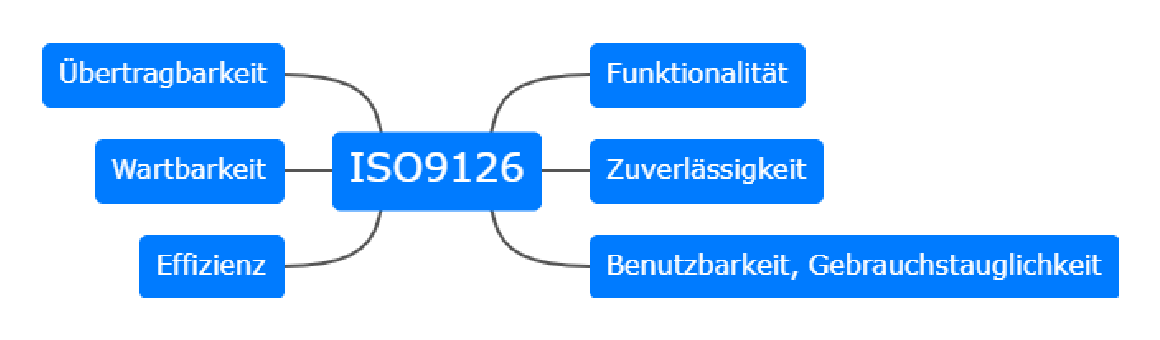
\includegraphics[width=\textwidth]{graphics/ISO-9126.pdf}
\caption[Qualitätskriterien nach ISO9126]{Qualitätskriterien nach ISO9126.\footnotemark}
\label{abb:ISO9126}
\end{figure}
\footnotetext{Mit Änderungen entnommen aus: \cite{Johner.2018}}


\pagebreak

\anhang{AWS Well Architected Referenzarchitekturen}
Folgend sind die Referenzarchitekturen aus dem \ac{AWS} Well Architected Framework - Analyticss Lens abgebildet.
\begin{figure}[H]
\centering
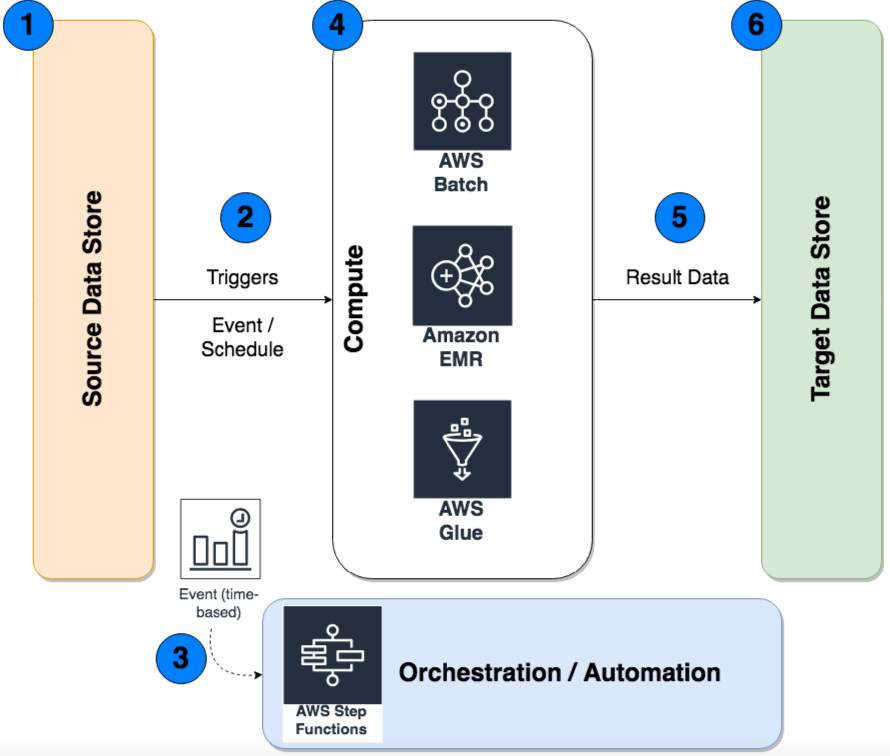
\includegraphics[width=\textwidth]{graphics/AWS-Batch-Architecture.pdf}
\caption[AWS Well Architected Batch Architektur]{AWS Well Architected Batch Architektur.\footnotemark}
\label{abb:AWSWellArchitectedBatch}
\end{figure}
\footnotetext{Entnommen aus: \cite[][12]{Ravirala.2020}}

\begin{figure}[H]
\centering
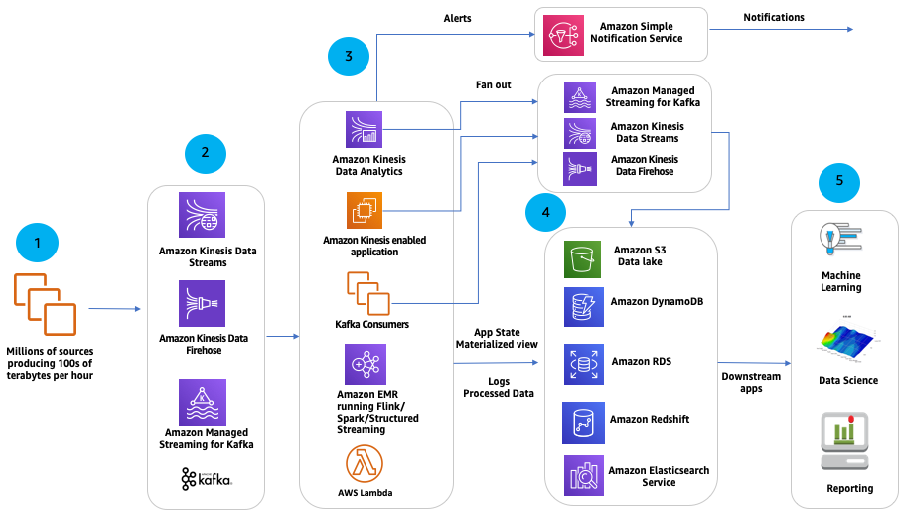
\includegraphics[width=0.92\textheight,angle=90,origin=c]{graphics/AWS-Stream-Architecture.pdf}
\caption[AWS Well Architected Stream/$\kappa$ Architektur]{AWS Well Architected Stream/$\kappa$ Architektur.\footnotemark}
\label{abb:AWSWellArchitectedStream}
\end{figure}
\footnotetext{Entnommen aus: \cite[][15]{Ravirala.2020}}

\begin{figure}[H]
\centering
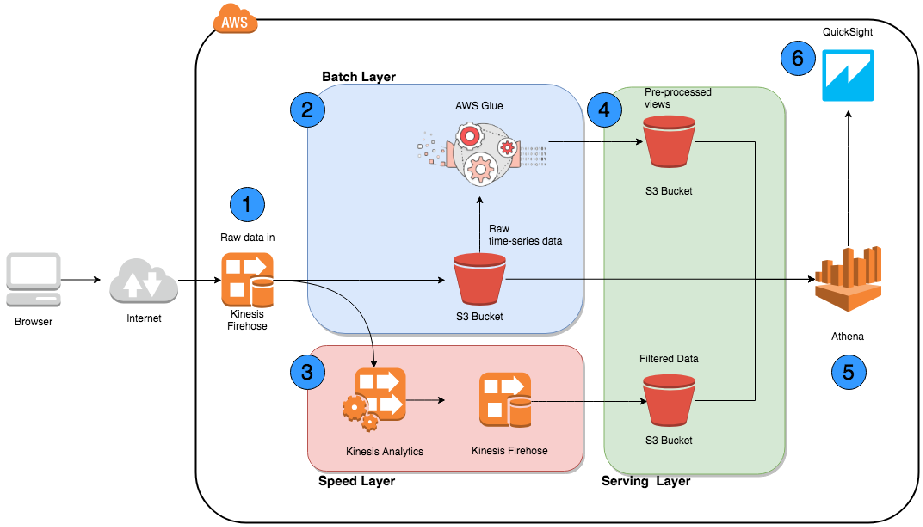
\includegraphics[width=0.92\textheight,angle=90,origin=c]{graphics/AWS-Lambda-Architecture.pdf}
\caption[AWS Well Architected $\lambda$ Architektur]{AWS Well Architected $\lambda$ Architektur.\footnotemark}
\label{abb:AWSWellArchitectedLambda}
\end{figure}
\footnotetext{Entnommen aus: \cite[][18]{Ravirala.2020}}

\anhang{Berechnungsskript Dateigröße}\label{anhang:berechnung}
Angefügt ist das verwendete Berechnungsskript für die Dateigröße, geschrieben in JavaScript, ausführbar mit der Node.JS Umgebung.

\begin{listing}[H]
\inputminted[frame=lines,breaklines=true]{javascript}{estimates/estimate.js}
\caption{Berechnungsskript Dateigröße}
\label{listing:js}
\end{listing}






% \anhangteil{Wieder mal eine Abbildung}\label{anhang:abbildung}
% \begin{figure}[htb]
% \centering
% 
\includegraphics[width=0.9\linewidth]{graphics/dhbw.png}
% \caption{Mal wieder das DHBW-Logo.}
% \end{figure}

% \anhangteil{Etwas Source Code}\label{anhang:sourcecode}
% \lstinputlisting{includes/HelloWorld.java}


%%% Ende des eigentlichen Inhalts %%%

\clearpage
\todos



%%% Quellenverzeichnisse (keine Anpassung nötig) %%%
\clearpage
\literaturverzeichnis
%%% Ende Quellenverzeichnisse %%%


%%% Erklärung (keine Anpassungen nötig) %%%
% steht ganz am Ende des Dokuments
\cleardoublepage
\clearpage

\thispagestyle{empty}

{\LARGE\textsf{\textbf{Erklärung}}\bigskip}

% \typMeinerArbeit und \themaMeinerArbeit werden in deckblatt.tex definiert
Ich versichere hiermit, dass ich meine \typMeinerArbeit\ mit dem Thema: \emph{\themaMeinerArbeit} selbstständig verfasst und keine anderen als die angegebenen Quellen und Hilfsmittel benutzt habe.
Ich versichere zudem, dass die eingereichte elektronische Fassung mit der gedruckten Fassung übereinstimmt.

\vspace{3cm}

\begin{center}
\begin{tabular}{ccc}
Rutesheim, 09.05.2021 &  & \\
(Ort, Datum) & \hspace{0.3\linewidth} & (Unterschrift)
\end{tabular}
\end{center}
\end{document}